% !TeX document-id = {283edc98-46be-43e5-9b77-8f898508d0c7}
% !TeX TXS-program:compile = txs:///pdflatex/[--shell-escape]
\documentclass[10pt,a4paper,hidelinks]{book}

\setcounter{secnumdepth}{0} %
\setcounter{tocdepth}{4} %per non numerare le section e subsection

\usepackage[stable]{footmisc} %per mettere caption nel titole delle section

\usepackage[T1]{fontenc}
\usepackage[utf8]{inputenc}
%\usepackage[italian]{babel}
\usepackage{amsmath}
\usepackage{pdfpages}
\usepackage{multicol}
\usepackage{placeins}
\usepackage{amsfonts}
\usepackage{booktabs}
\usepackage{amssymb}
\usepackage{graphicx}
\usepackage{caption}
\usepackage{subcaption}
\usepackage{siunitx}
\usepackage{hyperref}
\usepackage{subcaption}
\usepackage{wrapfig}
\usepackage{appendix}
\usepackage{xcolor}  % to access the named colour LightGray
\usepackage{easyReview}  % for \comment, \alert, etc.
\usepackage[most,breakable,skins]{tcolorbox} %crea box colorati per il testo
\usepackage[left=3cm,right=3cm,top=2cm,bottom=2.5cm]{geometry}
\newcommand{\HRule}[1]{\rule{\linewidth}{#1}}
\usepackage{minted}
\usemintedstyle{colorful}
\definecolor{LightGray}{gray}{0.97}

\newmintedfile[pythoncode]{python}{
frame=single,
framesep=2mm,
baselinestretch=1.2,
fontsize=\footnotesize,
linenos
 }
 
\setminted[python]{frame=single,
framesep=2mm,
baselinestretch=1.2,
fontsize=\footnotesize,
linenos}

\setminted[c]{frame=single,
	framesep=2mm,
	baselinestretch=1.2,
	fontsize=\footnotesize,
	linenos}

\setminted[bash]{frame=single,
framesep=2mm,
baselinestretch=1.2,
fontsize=\footnotesize,
bgcolor=LightGray,
linenos}

%\title{Computing Methods for Experimental \\ Physics and Data Analysis - Appunti}
%\author{Lorenzo Zaffina}
%\date{compilato il \today}
\begin{document}

\title{ \normalsize \textsc{Note del corso}
		\\ [0.2cm]
		\HRule{0.5pt} \\
		\LARGE \textbf{\uppercase{Computing Methods for Experimental Physics and Data Analysis}\\ [0.2cm]
		A.A. 2022-23}
		\HRule{2pt} \\ [0.5cm]
		\normalsize Compilato il \today \vspace*{5\baselineskip}}

\date{}

\author{
		Lorenzo Zaffina \\  [0.8cm]
		Università di Pisa \\ }



\maketitle



\tableofcontents

\chapter{Modulo Base - Scientifc Python}

\vfill
Per realizzare gli appunti su questa parte del corso, ho in gran parte utilizzato il materiale disponibile su al link \url{https://github.com/lucabaldini/cmepda.git}.

\newpage
\section{\textit{Lun 20 sett - Lezione 1}}
\section{Lecture basic 1: Development workflow}

\subsection{L'importanza della riproducibilità}
La ricerca scientifica dovrebbe essere prima di tutto \textit{corretta} e \textit{riproducibile}. In particolare, \textit{riproducibile} vuol dire che deve essere possibile, partendo dagli stessi dati, arrivare alle stesse conclusioni.\\
Il software ricopre un ruolo fondamentale nella moderna fisica sperimentale. Per questo motivo deve essere trattato alla stregua di un esperimento scientifico, cioè deve essere sviluppato in maniera controllata e deve essere riproducibile.




\subsection{Version control}

“Version control”: \textit{A component of software configuration
management, version control, also known as revision control or
source control, is the management of changes to documents,
computer programs, large web sites, and other collections of
information}\footnote{Wikipedia}\\

Un sistema di Version Control permette di raccogliere metadati\footnote{In informatica il metadato è un sistema strutturato di dati sui dati. Il suo scopo è di descrivere il contenuto, la struttura e l’ambito in cui s’inquadra un documento informatico, per la sua gestione e archiviazione nel tempo.} sul codice ogni qual volta il codice subisce delle modifiche.


\subsection{Terminologia}

  \begin{itemize}
  \renewcommand\labelitemi{--}
  \setlength\itemsep{0.1em}
  \item \textbf{Repository}: the place where files' current and historical data
    are stored
  \item \textbf{Revision or version}: the state at a point in time of the entire
    tree in the repository
  \item \textbf{Clone}: creating a repository containing the revisions from
    another repository
  \item \textbf{Working copy}: a local copy of files from a repository at a
    specific revision
  \item \textbf{Checkout}: create a local working copy from the repository
  \item \textbf{Change or diff}: a specific modification to a set of files under
    version control
  \item \textbf{Commit}: write the changes made in the working copy back to the
    repository
  \end{itemize}


\subsection{Tipologie di Version Control System}
Nel corso degli anni sono state sviluppate diverse tipologie di sistemi di controllo di configurazione. I principali sono i seguenti: \newpage


\subsection{Local version control systems (e.g. RCS)}


\begin{figure}[ht]
    \centering
    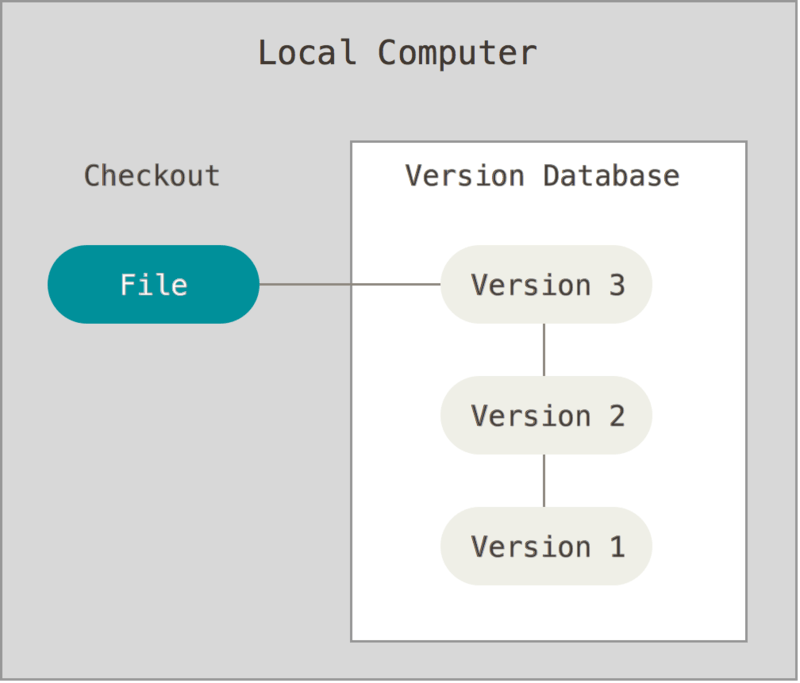
\includegraphics[width=0.5\textwidth]{lez1/localVCS.png}
    \caption{Local version control system: Keeps differences between revisions in a local database. Can recreate what any file looked like at any point in time. }
    \label{localVCS}
\end{figure}
\FloatBarrier


\subsection{Centralized Version Control Systems (e.g. CVS, Subversion)}

\begin{figure}[ht]
    \centering
    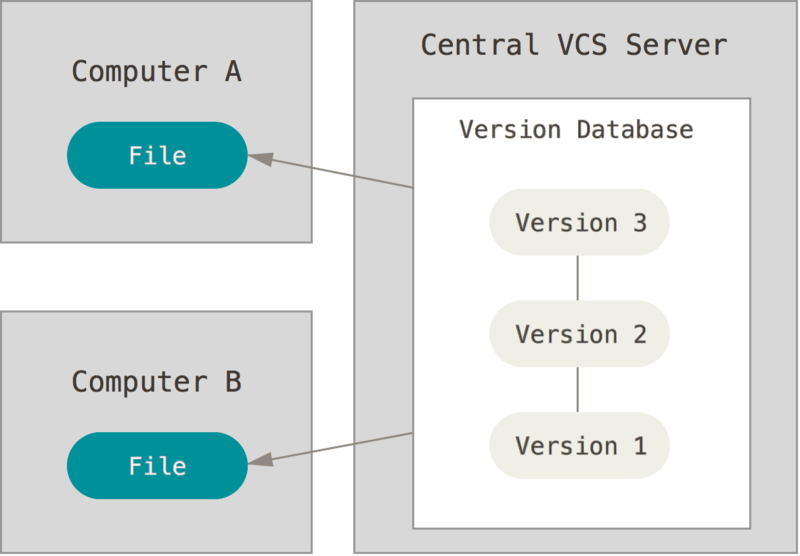
\includegraphics[width=0.5\textwidth]{lez1/centralVCS.png}
    \caption{Centralized Version Control System: Single server containing all the versioned files. Clients can check out the files from the repository. Most popular model through most of the ’90.}
    \label{centralVCS}
\end{figure}
\FloatBarrier

Il work-flow tipico dei Centralized Version Control System è molto basico:
\begin{enumerate}
    \setlength\itemsep{0.1em}
    \item Check out a local working copy from the remote server
    \item Modify the working copy
    \item Commit the changes back to the repository
\end{enumerate}

\newpage
\subsection{Distributed version control system (e.g. git, mercurial)}



\begin{figure}[ht]
    \centering
    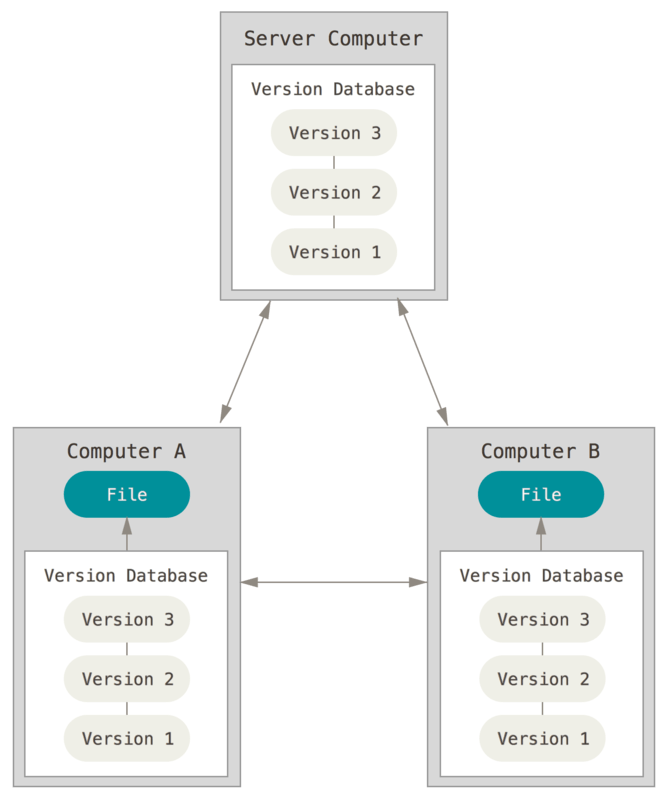
\includegraphics[width=0.5\textwidth]{lez1/distributedVCS.png}
    \caption{Distributed version control system: Clients fully mirror the repository, including its full history. Allows for a much richer variety of work-flows.}
    \label{distrVCS}
\end{figure}
\FloatBarrier


\subsection{Versioning single files vs. the entire repository}

Old VCS only tracked modification on a file-by-file basis; i.e., CVS assigns revision numbers to the single files.
All modern VCS track a whole commit as a new revision; i.e., revisions are assigned to the repository.\\
It makes a lot of sense to version the entire repository.
Versioning single files can give a cozy feeling, but when files interact with each other you need to know the status
of the entire repository to reliably predict the output!



\subsection{Centralized vs. distributed VCS}





\begin{figure}[ht]
    \centering
    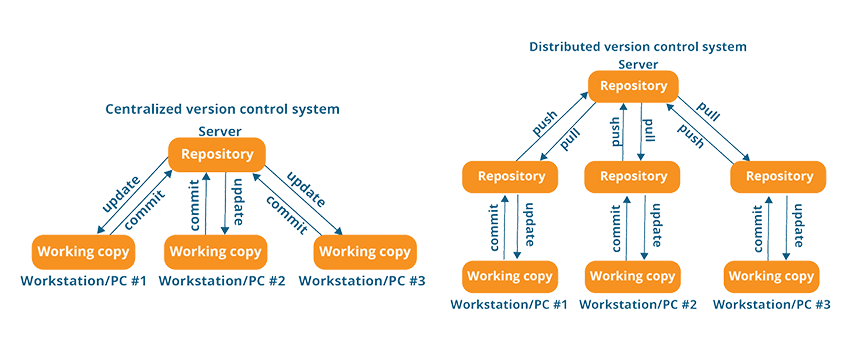
\includegraphics[width=1\textwidth]{lez1/centralvsdistr.png}
    \caption{Confronto tra un sistema di controllo centralizzato ed uno distribuito.}
    \label{confrontoVCS}
\end{figure}
\FloatBarrier

Il workflow nel caso del \textit{centralized VCS} è \textbf{lineare}: \textit{Subversion assigns a progressive number to the repo at each commit.}\\

Invece nel caso di un \textit{Distributed VCS}, il workflow è intrinsecamente \textbf{non lineare}: \textit{Any one given local repository is not ahead or behind any other
repository—just different.}\\
Ma allora come facciamo ad assegnare una versione (revision) in un sistema distribuito? Per capirlo facciamo una piccola digressione sulle funzioni di hash:

\subsection{Funzioni di Hash}

Nel linguaggio matematico e informatico, l'hash è una funzione non invertibile che mappa una stringa di lunghezza arbitraria in una stringa di lunghezza predefinita. Esistono numerosi algoritmi che realizzano funzioni hash con particolari proprietà che dipendono dall'applicazione.\footnote{Wikipedia}

\begin{figure}[ht]
    \centering
    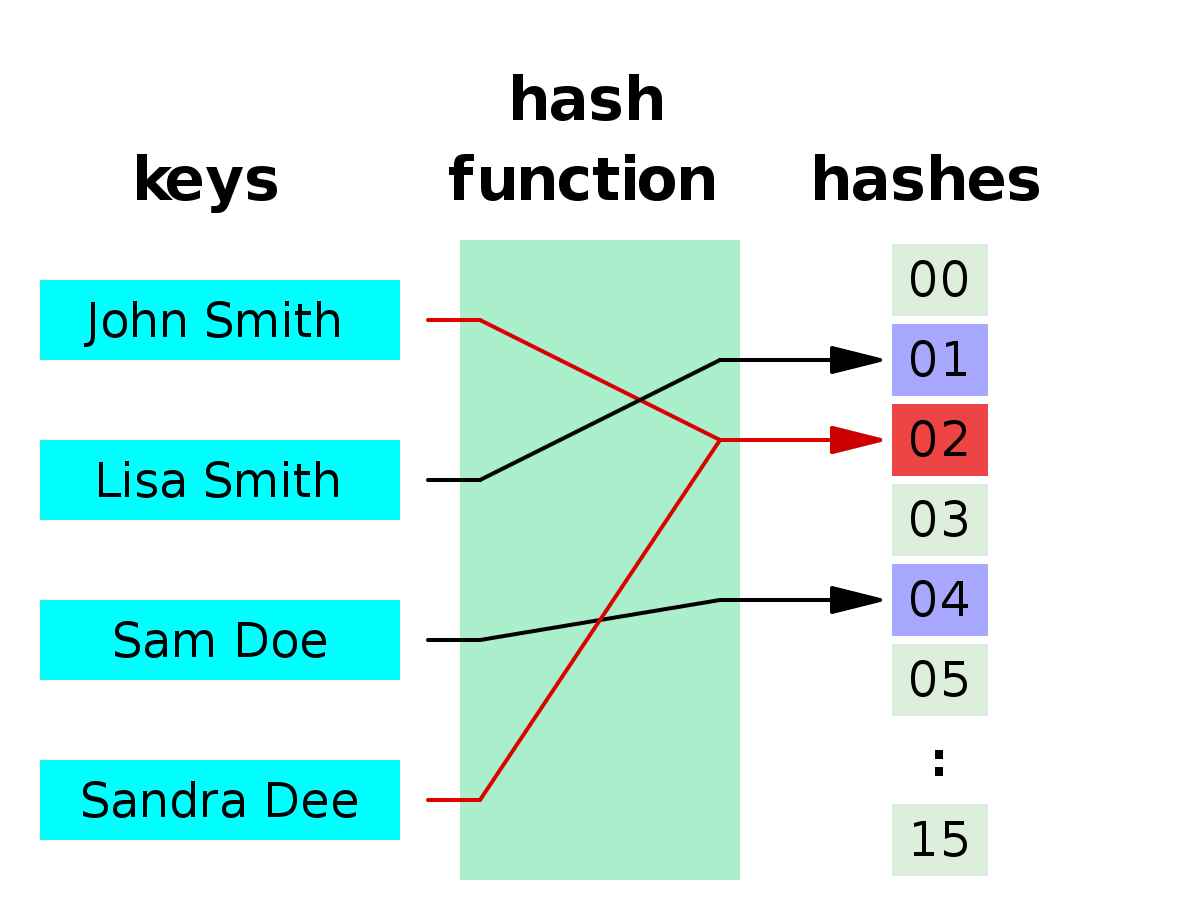
\includegraphics[width=0.5\textwidth]{lez1/hash.png}
    \caption{Esempio di funzione di hash.}
    \label{hash}
\end{figure}
\FloatBarrier


\textit{Hash function maps data of arbitrary size to fixed-size values (e.g., anything to an integer).}\\

Alcune proprietà che deve avere una buona funzione di hash:

\begin{itemize}
\renewcommand\labelitemi{--}
\setlength\itemsep{0.1em}
\item Deterministica.
\item Uniforme nello spazio immagine (minimicca le collisioni).
\item Facile da calcolare (e, possibilmente, difficile da invertire).
\end{itemize}


% \inputminted[frame=lines,framesep=2mm,bgcolor=LightGray]{python}{snippets/hashing.py}

\begin{minted}
[
frame=single,
framesep=2mm,
baselinestretch=1.2,
fontsize=\footnotesize,
linenos
]
{python}
print(hash(3))
print(hash(3.))
print(hash(3.001))
print(hash(’hello’))
print(hash(’Hello’))

[Output]
3
3
2305843009213443
-8080512805622017032
-8706679013462221575
\end{minted}

Every immutable object is hashable in Python. Each type gets its own algorithm.
This is important because in distributed VCS each commit gets its own hash.




\subsection{Altra Terminologia}

\begin{figure}[ht]
    \centering
    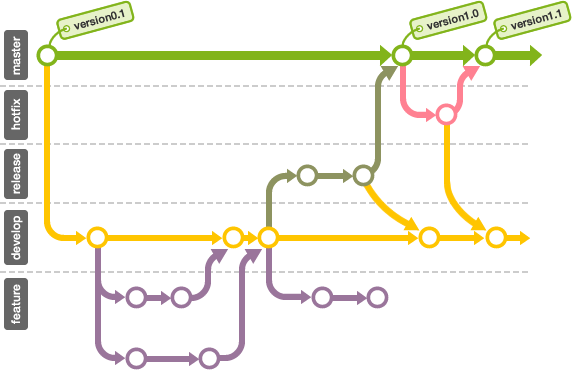
\includegraphics[width=0.5\textwidth]{lez1/branching.png}
    \caption{Esempio di branching.}
    \label{branching}
\end{figure}
\FloatBarrier


\begin{itemize}
  \renewcommand\labelitemi{--}
  \setlength\itemsep{0.1em}
  \item \textbf{Branches:} alternative paths where more copies of the same files develop in different ways independently.
  
  \item \textbf{Master, or trunk, or tip:} the unique line of development that is not a branch.
  
  \item \textbf{Merge:} application of two sets of changes to a set of files.
  \item \textbf{Conflict:} changes to the same file by two or more developers that
the system is unable to reconcile.
  \end{itemize}

\newpage
\section{\textit{Gio 22 sett - Lezione 2}}
\section{Lecture basic 2: Python Basics (1/2)}

\subsection{PEP: Python Enhancement Proposal}

\textit{"PEP stands for Python Enhancement Proposal, and there are several of them. A PEP is a document that describes new features proposed for Python and documents aspects of Python, like design and style, for the community."}

\subsection{Coding Conventions}
Ci sono delle linee guida su come scrivere il codice. Queste si chiamano \textit{Coding Conventions}, e differiscono per ogni linguaggio.\\
In particolare la \textbf{PEP8}\footnote{dargli un'occhiata \url{https://peps.python.org/pep-0008/}} codifica la coding convention in python.\\

Un esempio può essere quello di usare per le indentazioni gli spazi anziché i tab. Questo perché il tab dipende dall'editor di testo usato e questo è un male!\\

Esistono dei tool che permettono di controllare automaticamente quanto un codice è \textit{Pythonico}, ad esempio \textbf{pylint}\footnote{\url{https://www.pylint.org/}}.
\'E buona abitudine, prima di pushare un file su github, usare pylint per controllare che non ci siano errori nel codice!.


\subsection{Variables and basic types}
Python è quello che si chiama \textit{linguaggio tipizzato forte}\footnote{In un linguaggio fortemente tipizzato, il programmatore è tenuto a specificare il tipo di ogni elemento sintattico che durante l'esecuzione denota un valore (per esempio un valore costante, una variabile o un'espressione), e il linguaggio garantisce che tale valore sia utilizzato in modo coerente con il tipo specificato: per esempio, non è possibile eseguire una somma aritmetica su dati di tipo stringa. Questo concetto generale può applicarsi con diverse sfumature; a seconda del contesto.}.
Nonostante ciò, in python le variabili non si dichiarano. Posso scrivere:

\begin{minted}
[
frame=single,
framesep=2mm,
baselinestretch=1.2,
fontsize=\footnotesize,
linenos
]
{python}
x = 3
x = 'ciao'
\end{minted}

senza che mi dia errore.\\
Invece in C (così come nella maggior parte dei linguaggi compilati), una volta dichiarata una variabile, essa è di quel tipo per sempre!\\

Vediamo ora le principali strutture dati di python. Ricordiamo che le strutture dati si differenziano in mutabili e immutabili. In particolare, le strutture dati sono definite dalle operazioni che ci posso fare sopra.\\

\begin{itemize}
    \item \textbf{Numeri} (Interi, Float): notiamo che in python esiste un solo tipo di interi, detto "a precisione illimitata": posso rappesentare un numero arbitrariamente grande finché non finisco la RAM.\\
    \item \textbf{Stringhe}: è equivalente usare le virgolette singole (' ') o doppie (" ").
    
    \item \textbf{Liste}: le liste sono sequenze di elementi, che possono essere di qualsiasi tipo, anche liste stesse. Ad esempio posso accedere al primo elemento della lista \texttt{l} facendo \texttt{l[0]}; oppure cambiare un elemento facendo \texttt{l[0]='ciao'}. Infine posso appendere un elemento alla fine facendo \texttt{l.append('last')}.
    
    \item \textbf{Tuple}: ad esempio \texttt{t = (1,2,3)}. Una tupla è come una lista, ma è immutabile. Posso sempre accedere al primo elemento della tupla \texttt{t} facendo \texttt{t[0]}, ma \textbf{non} posso cambiare un elemento facendo ad esempio \texttt{l[0]=33}.\\
    Se scrivo su terminale: \texttt{(1,2,3)+(5,6,7)}, otterrò la nuova tupla \texttt{(1,2,3,5,6,7)}.
    \item \textbf{Dizionari}: Sono oggetti di tipo chiave-valore, ovvero mappano (mediante hash table o albero binario) una chiave in un valore. Sono efficienti nel trovare il valore associato alla chiave. Ad esempio \texttt{'a':3, 'b':4}.
\end{itemize}

Di seguito alcuni esempi:
\begin{minted}
[
frame=single,
framesep=2mm,
baselinestretch=1.2,
fontsize=\footnotesize,
linenos
]
{python}
i = 3
x = 3.0
print(i, type(i))
print(x, type(x))
s = ’Hi there!’
print(s, type(s))
l = [1, 2, ’a string’]
print(l, type(l), l[0])
t = (1, 2, ’a string’)
print(t, type(t), t[0])
d = {’key1’: 1, ’key2’: 2}
print(d, type(d), d[’key1’])
[Output]
3 <class ’int’>
3.0 <class ’float’>
Hi there! <class ’str’>
[1, 2, ’a string’] <class ’list’> 1
(1, 2, ’a string’) <class ’tuple’> 1
’key1’: 1, ’key2’: 2 <class ’dict’> 1
\end{minted}


\subsection{String Formatting}
\'E poco pithonico usare l'operatore \texttt{+} per unire due stringhe, facendo ad esempio \texttt{'Luca' + 'Baldini'}.\\
\'E anche preferibile evitare usare l'operatore \%.\\
La cosa migliore è usare le \textit{f-string}, come si vede nel seguente esempio:


\begin{minted}
[
frame=single,
framesep=2mm,
baselinestretch=1.2,
fontsize=\footnotesize,
linenos
]
{python}

name = 'Luca'
age = 42

# The ugly way.
print('My name is ' + name + ' I am ' + str(age) + ' year(s) old.')

# The old way (% operator)
print('My name is %s I am %d year(s) old.' % (name, age))

# The new way (.format)
# This is actually *much* more powerful and flexible than implied here.
print('My name is {} I am {} year(s) old.'.format(name, age))

# The newer way---new in Python 3.6. This is awesome!
print(f'My name is {name} I am {age} year(s) old.')


[Output]
My name is Luca I am 42 year(s) old.
My name is Luca I am 42 year(s) old.
My name is Luca I am 42 year(s) old.
My name is Luca I am 42 year(s) old.
\end{minted}

\subsection{Le Funzioni}

DRY (Don’t Repeat Yourself) is better than WET (Write Every Time). \'E importante dare un nome chiaro ed esplicativo alle funzioni che scriviamo.


\begin{minted}
[
frame=single,
framesep=2mm,
baselinestretch=1.2,
fontsize=\footnotesize,
linenos
]
{python}
import math
def square(x):
"""Return the square of x.
"""
return x * x
def cartesian_to_polar(x=1., y=1.):
"""Convert cartesian to polar coordinates.
"""
r = math.sqrt(x**2. + y**2.)
phi = math.atan2(y, x)
return r, phi
print(square(2.))
print(cartesian_to_polar(0., 1.))
print(cartesian_to_polar())
[Output]
4.0
(1.0, 1.5707963267948966)
(1.4142135623730951, 0.7853981633974483)
\end{minted}

\subsection{Funzioni Variadiche}
Sono delle funzioni che accettano un numero variabile di argomenti. Ad esempio:

\begin{minted}
[
frame=single,
framesep=2mm,
baselinestretch=1.2,
fontsize=\footnotesize,
linenos
]
{python}
import os
p1 = os.path.join(’path’, ’to’, ’my’, ’file’)
p2 = os.path.join(’howdy’, ’partner’)
print(p1)
print(p2)
s1 = sum([1, 2])
s2 = sum([1, 2, 3, 4, 5])
print(s1)
print(s2)
[Output]
path/to/my/file
howdy/partner
3
15
\end{minted}

\subsection{Arbitrary argument lists}

\begin{minted}
[
frame=single,
framesep=2mm,
baselinestretch=1.2,
fontsize=\footnotesize,
linenos
]
{python}
import os
def join1(*args):
"""Horrible: do not use the + operator with strings in a loop.
"""
out = ’’
for arg in args:
out += ’%s/’ % arg
return out.rstrip(’/’)
def join2(*args):
"""This a more sensible version---and you get the idea of the *.
"""
return ’/’.join(args)
def join3(*args, sep=os.path.sep):
"""Even better---this will work on any OS.
"""
return sep.join(args)
print(join1(’path’, ’to’, ’file’))
print(join2(’path’, ’to’, ’file’))
print(join3(’path’, ’to’, ’file’))
[Output]
path/to/file
path/to/file
path/to/file
\end{minted}

\subsection{Un esempio: la funzione di fit}

\begin{minted}
[
frame=single,
framesep=2mm,
baselinestretch=1.2,
fontsize=\footnotesize,
linenos
]
{python}
import numpy as np
import matplotlib.pyplot as plt
from scipy.optimize import curve_fit
x = np.linspace(0., 10., 11)
y = 2.5 + 3.2 * x
def model(x, m, q):
return m * x + q
popt, pcov = curve_fit(model, x, y)
plt.errorbar(x, y, fmt=’o’)
# Overlay the model without unpacking the best-fit parameters.
plt.plot(x, model(x, *popt))
# Compare with
# mhat, qhat = popt
# plt.plot(x, model(x, mhat, qhat))
\end{minted}

\subsection{Keyword arguments}
Keyword arguments (or named arguments) are values that, when passed into a function, are identifiable by specific parameter names. A keyword argument is preceded by a parameter and the assignment operator, = . Keyword arguments can be likened to dictionaries in that they map a value to a keyword.


\begin{minted}
[
frame=single,
framesep=2mm,
baselinestretch=1.2,
fontsize=\footnotesize,
linenos
]
{python}
def func(**kwargs):
"""
"""
print(kwargs.get(’verbose’, False))
func()
func(verbose=True)
func(verbose=False)
func(verbose=True, num_events=3)
func(True)
[Output]
False
True
False
True
Traceback (most recent call last):
File "snippets/func_kwargs.py", line 11, in <module>
func(True)
TypeError: func() takes 0 positional arguments but 1 was given
\end{minted}

\subsection{Basic control flow}

\begin{minted}
[
frame=single,
framesep=2mm,
baselinestretch=1.2,
fontsize=\footnotesize,
linenos
]
{python}
i = 2
# Conditional expressions
if i == 2:
print(’Apple’)
elif i == 3:
print(’Peach’)
else:
print(’Cheese’)
# For loops
for i in [1, 2, 3]:
print(i)
# While loops
while i != 0:
print(i)
i -= 1
[Output]
Apple
1
2
3
3
2
\end{minted}

\subsection{Advanced Iteration}

\begin{minted}
[
frame=single,
framesep=2mm,
baselinestretch=1.2,
fontsize=\footnotesize,
linenos
]
{python}
list1 = [’a’, ’b’, ’c’]
list2 = [10, 11, 12]
# Horrible (and very un-Pythonic, too)!
for i in range(len(list1)):
print(i, list1[i])
# Nice-looking.
for i, item in enumerate(list1):
print(i, item)
# Zipping iterables
for item1, item2 in zip(list1, list2):
print(item1, item2)
# List comprehension
print([x**2 for x in list2])
[Output]
0 a
1 b
2 c
0 a
1 b
2 c
a 10
b 11
c 12
[100, 121, 144]
\end{minted}

\subsection{Nota: I numeri in virgola mobile sono esatti}
Consideriamo il seguente esempio:
\begin{minted}
[
frame=single,
framesep=2mm,
baselinestretch=1.2,
fontsize=\footnotesize,
linenos
]
{python}
[lbaldini@nbbaldini slides]$ python

Python 3.7.4 (default, Jul 9 2019, 16:32:37)
[GCC 9.1.1 20190503 (Red Hat 9.1.1-1)] on linux
Type "help", "copyright", "credits" or "license" for more information.
>>> 0.1 + 0.2 == 0.3
False
>>> 0.2 + 0.2 == 0.4
True
\end{minted}

Cosa sta succedendo? Il fatto è che, essendo inesatti, non ha senso chiedere se due numeri in virgola mobile siano esatti!\\ Quando scriviamo un numero in virgola mobile, per il PC è sempre un numero raionale, in quanto è troncato.

\subsection{Rappresentazione in virgola mobile}
[...]

\subsection{References}

  \begin{itemize}
  \item\url{https://scipy-lectures.org/}
  \item\url{https://docs.quantifiedcode.com/python-anti-patterns/}
  \item\url{https://sebastianraschka.com/Articles/2014_python_2_3_key_diff.html}
  \item\url{https://www.python.org/dev/peps/pep-0020/}
  \item\url{https://www.python.org/dev/peps/pep-0008/}
  \item\url{https://docs.python-guide.org/writing/style/}
  \item\url{https://docs.python.org/3/library/stdtypes.html}
  \item\url{https://docs.python.org/3/tutorial/controlflow.html\#defining-functions}
  \item\url{https://docs.python.org/3/tutorial/floatingpoint.html}
  \item\url{https://floating-point-gui.de/}
  \item\url{https://www.itu.dk/~sestoft/bachelor/IEEE754_article.pdf}
  \end{itemize}

\section{Lecture basic 3: Python Basics (2/2)}

\subsection{La Python Standard Lybrary}

\begin{itemize}
  \item La gerarchia è sostanzialmtnete la seguente:
    \begin{itemize}
    \item The Python core language (all you get at the interpreter startup)
    \item The Python standard library (e.g., \texttt{math})
    \item An enourmous number of third-party packages (e.g., \texttt{numpy})
    \item Eventuali librerie scritte da noi
    \end{itemize}
  \item The standard library is included in every Python distribution
    \begin{itemize}
    \item And it is (slowly) evolving with time
    \end{itemize}
  \item With third-party packages you are on your own
    \begin{itemize}
    \item Although Anaconda solves many of the issues
    \item And if you are using GNU-Linux your package manager is probably
      taking care of everything for you
    \end{itemize}
  \item (Well---and of course there are your own modules, too\ldots)
  \item Anything that is out of the core is loaded in memory via an
    \texttt{import} statement
  \end{itemize}

\subsection{Il sistema di Import}

\begin{minted}
[
frame=single,
framesep=2mm,
baselinestretch=1.2,
fontsize=\footnotesize,
linenos
]
{python}
from math import *
[...]
# Terrible: where the hell is sqrt coming from?
x = sqrt(2.)
from math import sqrt
[...]
# Better: if you haven’t redefined sqrt this is from the math library
x = sqrt(2.)
import math
[...]
# Best: five more characters, but at least is clear where sqrt is coming from
x = math.sqrt(2.)
\end{minted}

  \begin{itemize}
  \item The \texttt{\$PYTHONPATH} environmental variables is your friend
    to control where you want to import modules from
    \begin{itemize}
    \item You will need to tweak it when you start writing your own packages
    \end{itemize}
  \item You will need suitable \texttt{\_\_init\_\_.py} files to navigate
    directories
  \end{itemize}

\textbf{Nota:} non abusare del sistema di import! Di seguito un esempio ok:

\begin{minted}
[
frame=single,
framesep=2mm,
baselinestretch=1.2,
fontsize=\footnotesize,
linenos
]
{python}
# This is ok, and vastly recognized by the community
import numpy as np
from matplotlib import pyplot as plt
x = np.linspace(0., 10., 100)
y = x**2.
plt.plot(x, y)
\end{minted}

Mentre il seguente esempio è una catastrofe!


\begin{minted}
[
frame=single,
framesep=2mm,
baselinestretch=1.2,
fontsize=\footnotesize,
linenos
]
{python}
from math import *
import logging as log
# ... 1000 lines of code in the middle
x = log(2.)
[Output]
Traceback (most recent call last):
File "snippets/import2.py", line 6, in <module>
x = log(2.)
TypeError: ’module’ object is not callable
\end{minted}

\subsection{La Standard Library: \texttt{time}, \texttt{datetime} and \texttt{calendar}}
\begin{itemize}
  \item Collections of facilities related to date and time
    \begin{itemize}
    \item Measure the execution time of your scripts
    \item Convert from time to date and vice-versa
    \end{itemize}
\end{itemize}
"Il tempo è una cosa seria" -Luca Baldini.

\subsection{La Standard Library: \texttt{math}}

\begin{minted}
[
frame=single,
framesep=2mm,
baselinestretch=1.2,
fontsize=\footnotesize,
linenos
]
{python}
Python 3.7.4 (default, Jul 9 2019, 16:32:37)
[GCC 9.1.1 20190503 (Red Hat 9.1.1-1)] on linux
Type "help", "copyright", "credits" or "license" for more information.
>>> import math
>>> dir(math)
[’__doc__’, ’__file__’, ’__loader__’, ’__name__’, ’__package__’, ’__spec__’,
’acos’, ’acosh’, ’asin’, ’asinh’, ’atan’, ’atan2’, ’atanh’, ’ceil’, ’copysign’,
’cos’, ’cosh’, ’degrees’, ’e’, ’erf’, ’erfc’, ’exp’, ’expm1’, ’fabs’,
’factorial’, ’floor’, ’fmod’, ’frexp’, ’fsum’, ’gamma’, ’gcd’, ’hypot’, ’inf’,
’isclose’, ’isfinite’, ’isinf’, ’isnan’, ’ldexp’, ’lgamma’, ’log’, ’log10’,
’log1p’, ’log2’, ’modf’, ’nan’, ’pi’, ’pow’, ’radians’, ’remainder’, ’sin’,
’sinh’, ’sqrt’, ’tan’, ’tanh’, ’tau’, ’trunc’]
>>>
\end{minted}
\textbf{Nota:} lavorando molto con gli array, ci troveremo ad usare principalmente \texttt{numpy} e \texttt{scipy}.

\subsection{La Standard Library: \texttt{random}}

\begin{minted}
[
frame=single,
framesep=2mm,
baselinestretch=1.2,
fontsize=\footnotesize,
linenos
]
{python}
Python 3.7.4 (default, Jul 9 2019, 16:32:37)
[GCC 9.1.1 20190503 (Red Hat 9.1.1-1)] on linux
Type "help", "copyright", "credits" or "license" for more information.
>>> import random
>>> print(dir(random))
[’BPF’, ’LOG4’, ’NV_MAGICCONST’, ’RECIP_BPF’, ’Random’, ’SG_MAGICCONST’,
’SystemRandom’, ’TWOPI’, ’_BuiltinMethodType’, ’_MethodType’, ’_Sequence’,
’_Set’, ’__all__’, ’__builtins__’, ’__cached__’, ’__doc__’, ’__file__’,
’__loader__’, ’__name__’, ’__package__’, ’__spec__’, ’_acos’, ’_bisect’, ’_ceil’,
’_cos’, ’_e’, ’_exp’, ’_inst’, ’_itertools’, ’_log’, ’_os’, ’_pi’, ’_random’,
’_sha512’, ’_sin’, ’_sqrt’, ’_test’, ’_test_generator’, ’_urandom’, ’_warn’,
’betavariate’, ’choice’, ’choices’, ’expovariate’, ’gammavariate’, ’gauss’,
’getrandbits’, ’getstate’, ’lognormvariate’, ’normalvariate’, ’paretovariate’,
’randint’, ’random’, ’randrange’, ’sample’, ’seed’, ’setstate’, ’shuffle’,
’triangular’, ’uniform’, ’vonmisesvariate’, ’weibullvariate’]
>>>
\end{minted}

Anche qui, useremo principalmente \texttt{numpy}.

\subsection{La Standard Library: \texttt{os}, \texttt{os.path}, \texttt{glob} and
    \texttt{shutil}}
Servono ad interagire con il sistema operativo:

\begin{itemize}
  \item Miscellaneous operating system interfaces
    \begin{itemize}
    \item Access filesystem (access, create and copy files and directories)
    \item List directory content
    \item Environmental variables
    \item Absolute and relative paths
    \item Exec OS commands
    \end{itemize}
  \item All of this in a cross-platform fashion!
  \end{itemize}

\subsection{La Standard Library: \texttt{argparse}}
\'E utilissimo per passare informazioni direttamente dalla linea di comando.
\begin{itemize}
  \item Ever found yourself modifying the source code and running your program with different parameters?
    \begin{itemize}
    \item This is a terribly bad practice!
    \item And git will complain about modified files :-)
    \end{itemize}
  \item Keep the argparse documentation under your pillow!
  \end{itemize}
    
    
\subsection{La Standard Library: \texttt{logging}}  
  \begin{itemize}
  \item Ever found yourself inserting debug print() statements in the code
    when needed?
    \begin{itemize}
    \item This is another terrible bad practice!
    \item And git will complain about modified files :-)
    \end{itemize}
  \item Imagine if there was a thing that:
    \begin{itemize}
    \item allowed to label messages with different levels of severity
      (e.g., debug, info, warning, error)
    \item dynamically set a global filter on the severity level
      (e.g., do not print debug messages)
    \end{itemize}
  \item This thing exists and is called \texttt{logging}
  \item Always prefer \texttt{logging} over \texttt{print}
  \end{itemize}

Esiste anche un altro modulo molto usato che si chiama \texttt{Loguru}. Permette anche di stampare i log su un \textbf{logfile}.

\subsection{Typical layout of a Python package} 
Say you have a project called sample:
\begin{minted}
[
frame=single,
framesep=2mm,
baselinestretch=1.2,
fontsize=\footnotesize,
linenos
]
{python}
README.rst
LICENSE
setup.py
requirements.txt
sample/__init__.py
sample/core.py
sample/helpers.py
docs/conf.py
docs/index.rst
tests/test_basic.py
tests/test_advanced.py
\end{minted}
\begin{itemize}
  \item Here is how the repository layout might look like:
    \begin{itemize}
    \item README.rst
    \item LICENSE (when in doubt use GPL v3)
    \item requirements.txt (dependencies, for pip)
    \item sample (actual python code, note it's the same name as the project)
    \item docs (documentation)
    \item tests (unit tests)
    \end{itemize}
  \item We shall talk a lot about installation, documentation and unit tests
    in the second part of the course (advanced Python)
  \end{itemize}

\subsection{References}
\begin{itemize}
  \item \url{https://docs.python.org/3/library/}
  \item \url{https://pypi.org/}
  \item \url{https://docs.python.org/3/reference/import.html}
  \item \url{https://docs.python-guide.org/}
  \item \url{https://docs.quantifiedcode.com/python-anti-patterns/}
  \end{itemize}

\newpage
\section{\textit{Gio 29 sett - Lezione 3}}
\section{Lecture basic 4: Algorithms and data structures}

Un algoritmo è una sequenza di istruzioni che dicono in modo \textbf{non ambiguo} come risolvere un problema.
Usare un algoritmo piuttosto che un altro può comportare una grande differenza in termini di efficienza di tempi.
\begin{itemize}
  \item Algorithms can be expressed in several different ways:
    \begin{itemize}
    \item Flowcarts
    \item Pseudo-code
    \item Working code snippets
    \end{itemize}
  \item The sequence of operation must be expressed \textbf{unambigously}
  \end{itemize}

\subsection{Esempio: ricerca sequenziale vs ricerca binaria}
\textbf{Problema: trovare un elemento in una lista ordinata.}\\
Posso fare 2 cose:\\
\textbf{1. Forza bruta:} Faccio un loop sulla lista finché non trovo (o no) l'elemento cercato. Questo diventa sempre più sconveniente man mano che la lista si allunga (se la lista è lunga N, in media dovrò controllare N/2 elementi).\\

\textbf{2. Ricerca Binaria:}
    \begin{itemize}
    \item Start from the middle (if that's the target you're done)
    \item If the target is smaller (larger) than the element in the center,
      bisect the half-list on the left (right)
    \item Iterate until you've found the target (or exhausted the list)
    \end{itemize}
In questo caso dovrò controllare in media $\log_2(n)$ elementi. \textbf{Il logaritmo fa una bella differenza!}\\


\subsection{Complessità di un algoritmo}
\textbf{Misura del costo computazionale di un algoritmo.} Lo quantifico come funzione della grandezza dell'input che noi diamo all'algoritmo. Per es se il nostro algoritmo agisce su una lista, è interessante vedere come scala il tempo di operazione in funzione della lunghezza della lista.\\
\textbf{Ordine di grandezza del numero di istruzioni elementari} è una buona stima del tempo di esecuzione del programma. (anche se le istruzioni elementari possono durare un po' diversamente da pc a pc e da linguaggio a linguaggio).\\
Il numero di istruzioni fondamentali che un algoritmo esegue dipende dai dati che gli diamo in ingresso (ad es, a parità di lunghezza della lista, dipende da come è ordinata la lista stessa). Posso comunque chiedermi cosa succede nel \textit{best case}, nel \textit{worst case} e in \textit{average}.

\begin{minted}
[
frame=single,
framesep=2mm,
baselinestretch=1.2,
fontsize=\footnotesize,
linenos
]
{python}
def find_maximum(list_):
"""Find the biggest element in a list.
"""
maximum = list_[0]
for value in list_[1:]:
if value > maximum:
maximum = value
return maximum

l = [1, 2, 5, 98, 3, 1672, 6, 34, 651]
print(find_maximum(l))

[Output]
1672
\end{minted}

  \begin{itemize}
  \item Example: find the largest element in a list of length $n$
  \item How many fundamental instructions is this code executing?
    \begin{itemize}
    \item \textcolor{teal}{(You should realize this is an ill-posed question)}
    \item One assignment and one list lookup at the beginning: $2$
    \item One lookup, one assignment and one comparison for each iteration
      in the for loop: $3(n - 1)$
    \item A variable number of assignments: between $0$ and $(n - 1)$
    \item One final return instruction: 1
    \end{itemize}
  \item \textcolor{teal}{Answer: anything between $3n$ and $4n - 1$}
    \begin{itemize}
    \item (Depending on the input list)
    \end{itemize}
  \end{itemize}

\begin{itemize}
  \item Message \#1: \textcolor{teal}{the exact number of fundamental instructions that an
    algorithm performs is not determined a priori}
    \begin{itemize}
    \item It depends on the input data, instead
    \item And so does the running time
    \end{itemize}
  \item There's a few questions that you can legitimetely ask, anyway
    \begin{itemize}
    \item How many instructions in the \textcolor{teal}{worst case}?
    \item How many instructions in the \textcolor{teal}{best case}?
    \item How many instructions on \textcolor{teal}{average}?
    \end{itemize}
  \item Message \#2: \textcolor{teal}{the \emph{exact} number of operations doesn't really
    matter}, does it?
    \begin{itemize}
    \item Different machines have different executions speed
    \item Different languages have different meaning of
      \emph{fundamental instruction}
    \end{itemize}
  \item Message \#3: still, \textcolor{teal}{the running time is related to the number
  of fundamental instructions}
  \end{itemize}

\subsection{Andamento asintotico e notazioni O-grandi}

\begin{itemize}
  \item Say you have an algorithm operating on an input of lenght $n$
    \begin{itemize}
    \item e.g., a list with $n$ elements
    \item or a string with $n$ characters 
    \end{itemize}
  \item How many fundamental instructions $N$ does it take to for your algorithm
    to run?
    $$
    N = f(n)
    $$
  \item \textcolor{teal}{Asymptotic behavior}: drop all the terms that grow slowly with
    $n$ and only keep the one that grows faster
    $$
    4n - 1 \approx 4n \quad\text{and}\quad 2n^2 + 6n + 3 \approx 2n^2
    $$
    (for large $n$)
  \item Let's go one step further, and say that we neglect the multiplicative
    factor in front of the leading term (posso ignorare il fattore moltiplicativo perché tanto non c'è una corrispondenza 1 ad 1 tra il numero di op elementari e il tempo).
    $$
    4n - 1 \approx n \quad\text{and}\quad 2n^2 + 6n + 3 \approx n^2
    $$
  \item \textcolor{teal}{big-O notation}: the two algorithms are $O(n)$ and $O(n^2)$
  \end{itemize}



\textbf{NB:} Se un algoritmo ha complessità $n^2$
se ho un input 10 volte più grande, il tempo impiegato sarà 100 volte più grande. (\textbf{un algoritmo di complessità $n^2$ fa schifo})


\begin{figure}[ht]
    \centering
    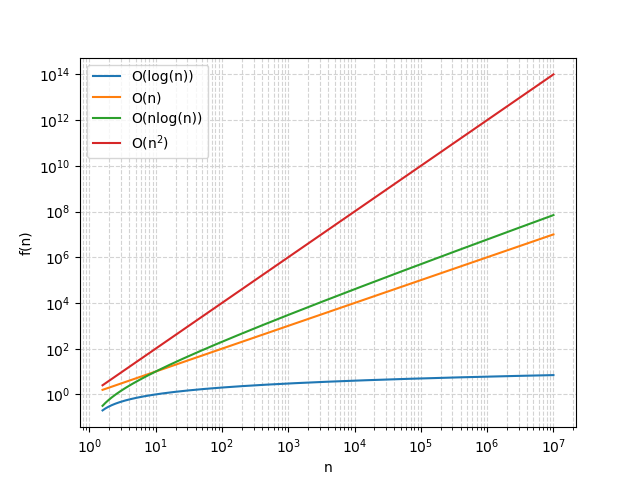
\includegraphics[width=0.8\textwidth]{lez3/asymptotic_behavior.png}
    \caption{Andamenti asintotici di vario tipo. If $n = 10^6$ and you can beat down the complexity from $n^2$ to $n\log(n)$ you are cutting down the execution time by one million!}
    \label{asympt}
\end{figure}
\FloatBarrier

\subsection{Come misuro il comportamento asintotico?}
Soprattutto in casi in cui ci sono un sacco di linee di codice.
\begin{itemize}
    \item \textbf{Forza Bruta}
        \begin{itemize}
        \item Implement the algorithm
        \item Run it on input data of different size and time the run
        \item (Be careful: results may vary from run to run)
        \item Plot the running time vs. input size
    \end{itemize}
    \item \textbf{Per Analisi}:
        \begin{itemize}
        \item Go ahead and count the instructions
        \item Evaluate the best, worst and average case
        \item (This can be difficult for complex programs, and subject to the
      hidiosyncrasis of the language)
    \end{itemize}

    \item \textbf{Ad Occhio}
        \begin{itemize}
        \item un loop ha tipicamente un costo O(n)
        \item anche due loop consecutivi hanno costo O(n)
        \item due loop annidati hanno un costo O($n^2$) appena vedo due loop annidati è un cattivo segno! A volte non si possono evitare, a volte sì!
        \end{itemize}
\end{itemize}


Una lettura leggera sulla "Complexity of Songs": \url{http://www.cs.bme.hu/~friedl/alg/knuth_song_complexity.pdf}

\subsection{Strutture dati: le liste}

\begin{figure}[ht]
    \centering
    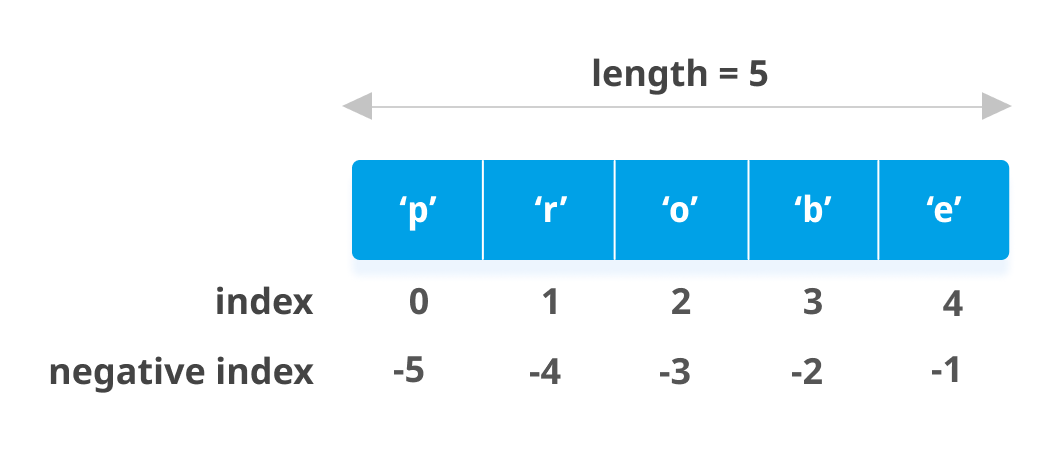
\includegraphics[width=0.7\textwidth]{lez3/list.png}
    \caption{ }
    \label{list}
\end{figure}
\FloatBarrier

\begin{center}

\begin{tabular}{lll}
    \hline
    Operation & Average case & Worst case\\
    \hline
    \hline
    Copy & O(n) & O(n)\\
    Append & O(1) & O(1)\\
    Insert & O(n) & O(n)\\
    Get Item & O(1) & O(1)\\
    Set Item & O(1) & O(1)\\
    Delete Item & O(n) & O(n)\\
    Iteration & O(n) & O(n)\\
    min(s), max(s) & O(n) & \\
    Get Length & O(1) & O(1)\\
    \hline
  \end{tabular}
\end{center}

Quando tolgo un elemento, una volta tolto devo poi rispostare tutto il resto! Per questo ho O(n).
\subsection{Hash table}



\begin{figure}[ht]
    \centering
    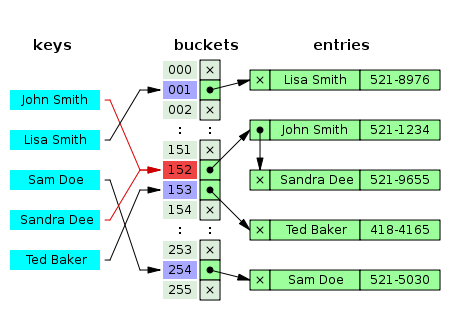
\includegraphics[width=0.7\textwidth]{lez3/hash.png}
    \caption{Hash table}
    \label{hash_table}
\end{figure}
\FloatBarrier

\begin{itemize}
  \item Associative array mapping keys to values
  \item Basic idea:
    \begin{itemize}
    \item Pre-allocate some space (which might grow or shrink)
    \item Keys are mapped to indices via a hash function
    \item This is about it, except that you have to be able to handle collisions
    \end{itemize}
  \item Hash tables (aka dictionaries) are highly optimized in Python
  \end{itemize}

\subsection{Strutture dati: I dizionari}


\begin{figure}[ht]
    \centering
    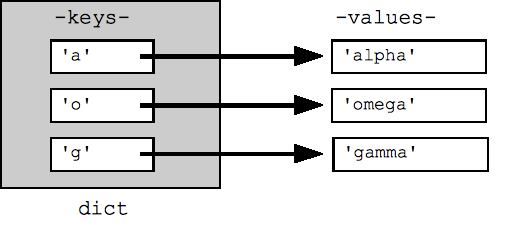
\includegraphics[width=0.6\textwidth]{lez3/dict.png}
    \caption{Dizionario}
    \label{dict}
\end{figure}
\FloatBarrier

\begin{center}

\begin{tabular}{lll}
    \hline
    Operation & Average case & Worst case\\
    \hline
    \hline
    Copy & O(n) & O(n)\\
    Get Item & O(1) & O(n)\\
    Set Item & O(1) & O(n)\\
    Delete Item & O(1) & O(n)\\
    Iteration & O(n) & O(n)\\
    \hline
  \end{tabular}
    
\end{center}

Per prendere un elemento, se non ci sono conflitti mi basta calcolare la funzine di hash sulla chiave. Ma se ci sono dei conflitti, nel caso peggiore in cui la struttura è piena, avrò n conflitti O(n).\\
I dizionari brillano nell'inserzione e nella cancellazione. I dizionari sono ottimi per i contesti in cui devo spesso inserire e/o cancellare cose.

\begin{minted}
[
frame=single,
framesep=2mm,
baselinestretch=1.2,
fontsize=\footnotesize,
linenos
]
{python}
print(hash(3))
print(hash(3.))
d = {}
d[3] = ’Hi there!’
print(d)
d[3.] = ’How are you?’
print(d)

[Output]
3
3
3: ’Hi there!’
3: ’How are you?’
\end{minted}


\begin{itemize}
\item When a float corresponds to an integer, its hash is the same as that of the integer
\item The hash is used to map keys into indices
\item Therefore: $3$ and $3.$ are the same key to a dictionary
\end{itemize}

\subsection{Sorting}
Programma che data una lista di numeri in virgola mobile, mi restituisce un'altra lista con gli stessi elementi, ma in ordine.\\

\begin{minted}
[
frame=single,
framesep=2mm,
baselinestretch=1.2,
fontsize=\footnotesize,
linenos
]
{python}
def sloppy_sort(list_):
"""Poor man’s implementation of a sorting algorithm.
"""
sorted_list = []
for item in list_:
if len(sorted_list) == 0:
sorted_list.append(item)
else:
if item < sorted_list[0]:
sorted_list.insert(0, item)
else:
for i, sorted_item in enumerate(sorted_list):
if item <= sorted_item:
sorted_list.insert(i, item)
break
return sorted_list
l = [10, 1, 5, 2, 7, 3, 9, 4]
print(l)
print(sloppy_sort(l))
[Output]
[10, 1, 5, 2, 7, 3, 9, 4]
[1, 2, 3, 4, 5, 7, 9, 10]
\end{minted}
Questo è un esempio molto brutto per un sort. Infatti contiene 2 for annidati, che corrispondono ad una complessità di ordine $O(n^2)$ (che fa schifo).\\

Esistono diversi algoritmi di sort, di seguito alcuni esempi:
\begin{figure}[ht]
    \centering
    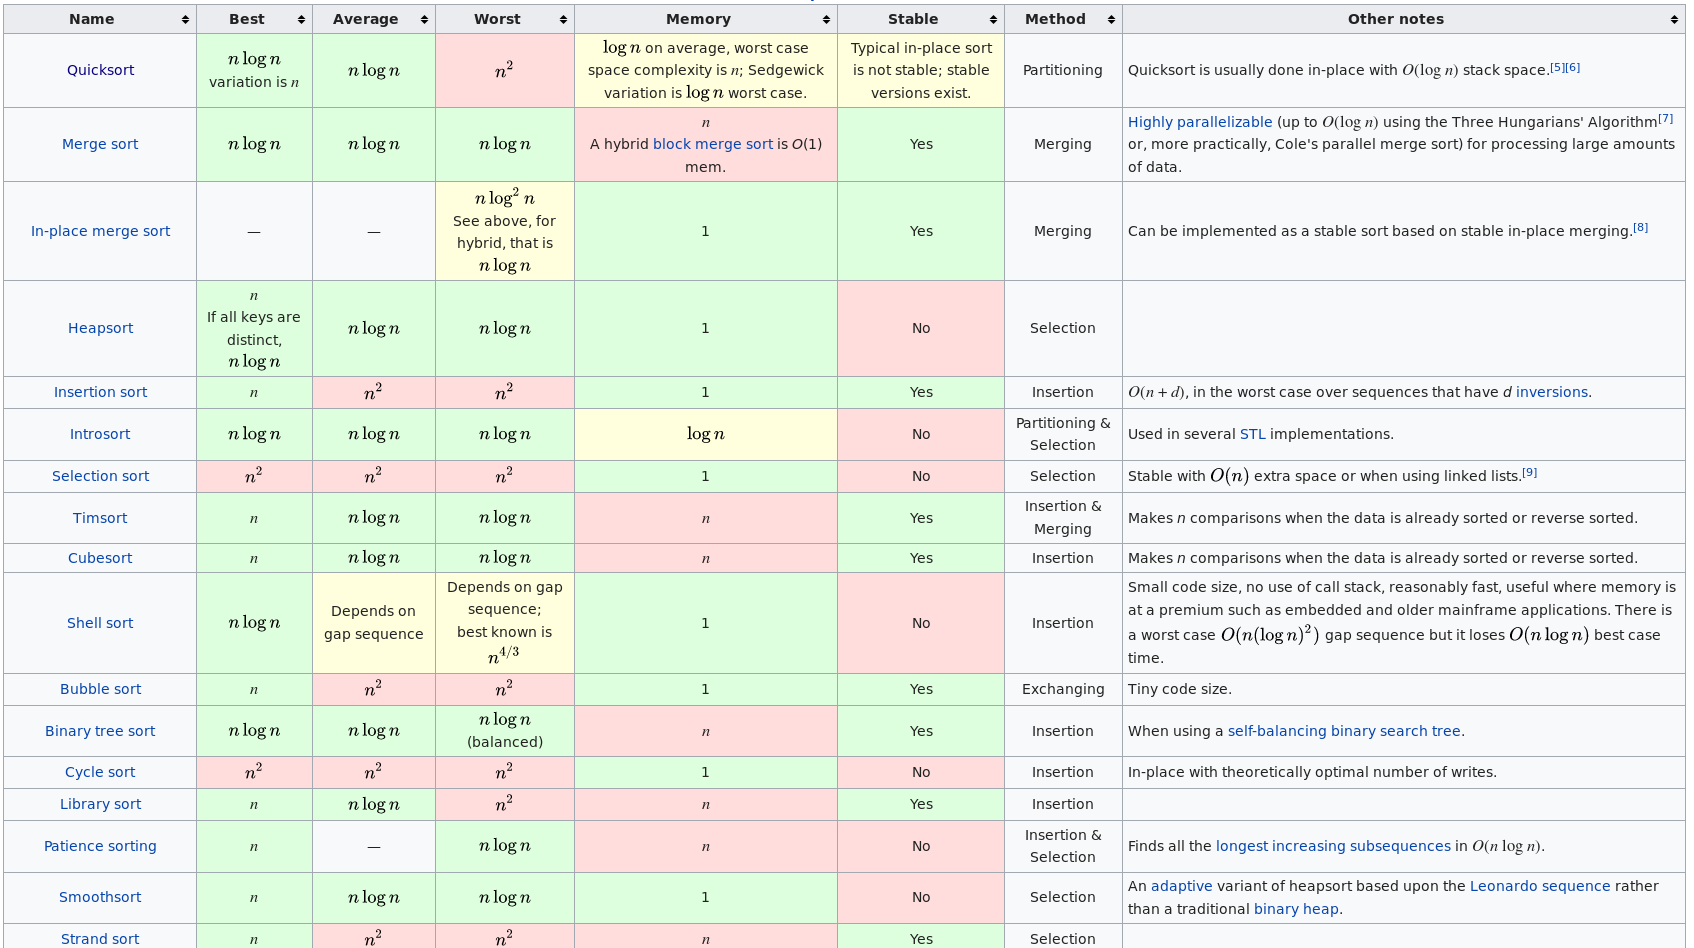
\includegraphics[width=1\textwidth]{lez3/sort.png}
    \caption{Alcuni algoritmi di sort, tabella presa dalla pagina di Wikipedia \url{https://en.wikipedia.org/wiki/Sorting_algorithm}}
    \label{sort}
\end{figure}
\FloatBarrier


Python come algoritmo di sort usa \textbf{Timsort}:
% (comando \texttt{sorted(list)})

\begin{minted}
[
frame=single,
framesep=2mm,
baselinestretch=1.2,
fontsize=\footnotesize,
linenos
]
{python}
l = [10, 1, 5, 2, 7, 3, 9, 4]
print(l)
l.sort()
print(l)

[Output]
[10, 1, 5, 2, 7, 3, 9, 4]
[1, 2, 3, 4, 5, 7, 9, 10]
\end{minted}
\begin{itemize}
  \item Hybrid algorithm, derived from merge sort and insertion sort
    \begin{itemize}
    \item Find subsequences of the data that are already ordered
    \item Use that knowledge to sort the remainder more efficiently
    \end{itemize}
  \item ``Although practicality beats purity'' (The Zen of Python)
  \end{itemize}


\subsection{References}
  \begin{itemize}
  \item \url{https://en.wikipedia.org/wiki/Algorithm}
  \item \url{https://discrete.gr/complexity/}
  \item \url{https://wiki.python.org/moin/TimeComplexity}
  \item \url{https://en.wikipedia.org/wiki/Sorting_algorithm}
  \item \url{https://bugs.python.org/file4451/timsort.txt}
  \item \url{https://en.wikipedia.org/wiki/Timsort}
  \end{itemize}

\section{Lecture basic 7: Numpy e Scipy}



  \begin{itemize}
    \item Among (many) other things, numpy offers:
    \begin{itemize}
    \item a powerful n-dimensional array object
    \item mathematical functions that interoperate natively with arrays
    \end{itemize}
  \item And scipy provides:
    \begin{itemize}
    \item integration
    \item optimization (a.k.a. fitting)
    \item interpolation
    \item signal processing
    \end{itemize}
  \end{itemize}

\subsection{Array di numpy}
Numpy fornisce un'implementazione efficiente di array.\\

Che differenza c'è tra una lista di python e gli array di numpy?
La prima differenza fondamentale è che gli array di numpy sono tendenzialmente \textbf{omogenei} (dentro lo stesso array non posso mescolare due tipi).\\

 
%\pythoncode{snippets/numpy_arrays.py}

\begin{minted}{python}
import numpy as np
# Initialization from a list
a1 = np.array([1., 2., 3])
print(a1)
# Zeros, ones, and fixed values
a2 = np.zeros(10)
a3 = np.ones((2, 2))
a4 = np.full(7, 3.)
print(a2)
print(a3)
print(a4)
# Grids
a5 = np.linspace(0., 10., 11)
a6 = np.logspace(0., 1., 11)
print(a5)
print(a6)

[Output]
[1. 2. 3.]
[0. 0. 0. 0. 0. 0. 0. 0. 0. 0.]
[[1. 1.]
 [1. 1.]]
[3. 3. 3. 3. 3. 3. 3.]
[ 0. 1. 2. 3. 4. 5. 6. 7. 8. 9. 10.]
[ 1.        1.25892541 1.58489319 1.99526231 2.51188643 3.16227766
3.98107171 5.01187234 6.30957344 7.94328235 10.      ]
\end{minted}

Altro esempio: \texttt{a = np.linspace(1, 10, 10, dtype=int)}\\
\noindent   
Se so che tipo di dati contiene un array, so già in partenza quanta memoria occupa. Questi array di numpy, una volta stanziati, tipicamente mantengono le stesse dimensioni.
\subsection{numpy arrays vs. Python lists}

\begin{minted}{python}
import numpy as np
# arrays and lists seem similar...
l = [1., 2., 3.]
a = np.array(l)
print(l)
print(a)
# ...but they support basic arithmetic in a different fashion
print(l + l)
print(a + a)

[Output]
[1.0, 2.0, 3.0]
[1. 2. 3.]
[1.0, 2.0, 3.0, 1.0, 2.0, 3.0]
[2. 4. 6.]
\end{minted}

 \begin{itemize}
  \item arrays and lists are fundamentally different objects
    \begin{itemize}
    \item different footprint in memory, operate at different speed
    \item arrays are homogeneous, lists don't need to
    \item arrays offer a much more powerful indexing/slicing
    \item arrays interoperate with numpy mathematical functions
    \end{itemize}
  \end{itemize}
  
\subsection{Broadcasting}
Broadcast vuol dire che su questi array posso fare delle operazioni (ad es somma di due array di stessa lunghezza).\\

\begin{minted}{python}
import numpy as np
a1 = np.array([1., 2.])
a2 = np.array([[1., 2.], [3., 4.]])
c = np.pi
print(a1)
print(a2)
print(c)
print(a1 * a1)
print(a1 * c)
print(a1 * a2)
[Output]
[1. 2.]
[[1. 2.]
[3. 4.]]
3.141592653589793
[1. 4.]
[3.14159265 6.28318531]
[[1. 4.]
[3. 8.]]
\end{minted}
Under certain conditions, numpy can make operations on arrays of different shape. This is extremely useful when vectorizing problems.\\

Con numpy posso fare cose fantasmagoriche del tipo:\\

\begin{minted}{python}
c = np.array([[1,2],[3,4]]\\
c = np.linspace(1,16,16).reshape((4,4))
\end{minted}

\textbf{Nota:} Ogni volta che operiamo su array, l'operazione avviene in C (perché il C è molto più veloce di python).
Sostituire un loop esplicito in python con un operazione tra array di numpy è una cosa ottima in termini di efficienza! Questa cosa si chiama \textbf{vettorizzazione}.\\
Consideriamo il seguente ciclo for:\\

\begin{minted}{python}
for v1, v2 in zip(v1, v2):
s += vi * v2}
\end{minted}


\noindent
dove \texttt{zip( , )} serve per looppare in contemporanea su due cose.\\
Posso fare la stessa operazione usando gli array di numpy:\\

\begin{minted}{python}
s = (v1 * v2).sum()
\end{minted}


\textbf{Ho vettorizzato il problema}. Cioè sono passato da un ciclo for ad un'operazione tra array. Ho ritrovato la velocità del C, mantenendo l'usabilità di python!

\newpage
\section{\textit{Lun 3 ott - Lezione 4}}

\section{Lecture basic: 5 - OOP\footnote{In informatica, la programmazione orientata agli oggetti (in inglese object-oriented programming, in acronimo OOP) è un paradigma di programmazione che permette di definire oggetti software in grado di interagire gli uni con gli altri attraverso lo scambio di messaggi. Particolarmente adatta nei contesti in cui si possono definire delle relazioni di interdipendenza tra i concetti da modellare (contenimento, uso, specializzazione), un ambito che più di altri riesce a sfruttare i vantaggi della programmazione ad oggetti è quello delle interfacce grafiche.} introduction (1/2)}


Una variabile, ad esempio un intero, funge da contenitore per un dato. Ci sono delle strutture dati, come liste e dizionari, che, oltre a contenere dei dati, sono caratterizzate da un set di operazioni che posso fare su di esse.\\

  \begin{itemize}
    \item Working with containers like lists or dictionaries, you may have noticed
          that they can do many thing besides holding the data
    \medskip
    \begin{itemize}
      \item You can extend a list using append() or insert()
      \item Trying to access a non-existent index in a list triggers a specific errror (\emph{IndexError})
      \item You can iterate on a list using the handy for-loop Python syntax
      \item and so on\dots
     \end{itemize}
     \medskip
     \item In other words, a list is a variable that, in addition to its data,
           shows some kind of specific \emph{behaviour}.
     \medskip
     \item How is that implemented?
  \end{itemize}


Si creano delle entità di codice (ogetti) che uniscono ai dati delle funzionalità per operare su di essi. Quindi non solo definiscono come è fatto quel dato in memoria, ma anche come si manipola quel dato.\\
L'idea di base è tenere il codice che opera su i dati e i dati stessi in un unica entià: \textbf{l'oggetto.}\\

Un oggetto è un'entità di codice caratterizzata da:
\begin{itemize}
    \item \textbf{Stato} $\rightarrow$ dati (attributi o membri)
    \item \textbf{Comportamento} $\rightarrow$ implementato tramite funzioni (metodi)
\end{itemize}

La programmazione a oggetti è usatissima, anche se non ovunque. Ad esempio il C non fa uso di programmazione ad oggetti.Comunque, quasi tutti i più importanti linguaggi di programmazione supportano la programmazione ad oggetti.\\

\subsection{Classi e Oggetti}

Una classe è un pezzo di codice che descrive come è fatto un oggetto. Se vogliamo programmare a oggetti dobbimo scrivere delle classi che permettono poi di creare degli oggetti.\\
Una classe è una generalizzazione del concetto di tipo. Ad es. il tipo "intero" si limita a dire quanto spazio occupa in memoria.\\ Quando scriviamo una classe dobbiamo anche descrivere le sue funzionalità (definendo delle funzioni).
Una volta che abbiamo la nostra classe, ad esempio \texttt{"studente"}, possiamo creare uno o più oggetti di tipo \texttt{"studente"}.\\

  \begin{itemize}
  \item Basic defnitions:
    \begin{itemize}
    \item A \alert{class} is a blueprint for creating objects
    \item An \alert{object} is a concrete relization of a class
    \end{itemize}

  \smallskip
  
  \item You can imagine a class like a project, which is used to
        describe how objects are built and how they works

  \smallskip

  \item You can have multiple objects of the same class
  
  \smallskip
  
  \item The relationship is similar to the one between types and variables:
    \begin{itemize} 
    \item A type is an abstract concept, describing how a varibale is
          represented in memory
    \item A variable is a concrete realization of it
    \item You can have several variables of the same type (like several integers
          or several strings)
    \end{itemize}
  
  \smallskip
  
  \item Indeed, to some extent, a class is the generalization of the concept of
        type. It specifies not only how an object \emph{is made} but also how \emph{it behaves}.
  \end{itemize}

\subsection{Esempio: creiamo la classe \texttt{televisione}
}

  \begin{itemize}
  \item Let's consider a familiar object, like a television. It has:
    \smallskip
    \begin{itemize}
    \item A state
      \begin{itemize}
      \item On/off (and possibly standby)
      \item Currently displayed channel
      \item Volume
      \item Brightness, contrast, etc\dots
      \end{itemize}

    \medskip
    
    \item A behaviour
      \smallskip
      \begin{itemize}
      \item Pressing the `power' button will turn ON/OFF
      \item Rotating the volume knob will increase/decrease the volumne
      \item Using the buttons on the remote control will change displayed 
            channel, brightness, contrast etc\dots
      \item And don't forget you need to plug-in before use!
      \end{itemize}
    \end{itemize}
  \end{itemize}

  \begin{itemize}
    \item How would that be represented in the code?
    \smallskip
      \begin{itemize}
      \item The state can be represented by some \alert{attributes} (variables):
      \begin{itemize}
        \item A boolean can represent the ON/OFF state
        \item For the currently displayed channel you can use an integer
        \item Volume, contrast, luminosity etc\dots they all get their own variable(s)
      \end{itemize}

      \medskip
    
      \item The behaviour can be implemented through the \alert{methods}:
      \smallskip
      \begin{itemize}
        \item For example the turn\_on() and turn\_off() functions may change the value of the variable
              and also produce all the related changes (i.e. start/stop video and audio) 
        \item You will probably have the netx\_channel() and previous\_channel() functions for zapping and so on\dots
        \item Of course it can be much more complex than that!
      \end{itemize}
    \end{itemize}
    
    \medskip
    
    \item Attributes and methods are collectively called \alert{members} of the class
    \medskip
    \item Each object of a specific class is an \alert{instance} of that class
  \end{itemize}


%Attributi e metodi si chiamano membri.\\
%Ogni oggetto di una classe specifica è un'\textit{istanza} di quella classe.

\subsection{Python Classes}

Convenzione: le classi le scrivo con l'iniziale maiuscola.\\


\inputminted{python}{snippets/class_tv_basic.py}

\begin{minted}{bash}
[Output]
<class ’__main__.Television’>
True

\end{minted}

In python tutti i tipi sono anche classi. Non esistono tipi di bassissimo livello.\\
Persino le funzioni sono classi.

\inputminted{python}{snippets/everything_is_a_class.py}

\begin{minted}{bash}
[Output]
<class ’int’>
<class ’str’>
<class ’list’>
<class ’function’>
\end{minted}


\subsection{Metodi}
Per definire un metodo, basta definire una funzione dentro una classe.\\
Tutti i metodi di una classe ricevono automaticamente come primo argomento l'oggetto su cui li chiamiamo (\texttt{self}).\\

\inputminted{python}{snippets/class_methods.py}

\begin{minted}{bash}
[Output]
Turning on <__main__.Television object at 0x7fc718217470>
Showing channel 3
\end{minted}

\subsection{Attributi}


\inputminted{python}{snippets/class_attributes_1.py}

\begin{minted}{bash}
[Output]
1
Traceback (most recent call last):
File "snippets/class_attributes_1.py", line 13, in <module>
print(another_tv.x)
AttributeError: ’Television’ object has no attribute ’x’
\end{minted}

\inputminted{python}{snippets/class_attributes_2.py}

\begin{minted}{bash}
[Output]
1
1
\end{minted}

\subsection{Costruttore}

  \begin{itemize}
    \small
    \item Adding attributes like that would be crazy\dots what would happen if I forgot
          to call the 'add\_a\_class\_attribute()' method in the previous example?
    \medskip
    \item Luckily there is a solution for that: the class \alert{constructor}
    \medskip
    \item The constructor is a special method that is called automatically each time
          a class instance is created
    \medskip
    \item A specificity of the constructor is that it cannot return anything
    \medskip
    \item In Python the constructor is the \emph{\_\_init\_\_} method%
          \footnote{Actually the real constructor -- that is the function responsible for 
                    creating the class instances -- is the \emph{\_\_new\_\_} operator, but 99\% of the time you don't need
                    to define that, as all classes have a default one which does the job for you}           
    \medskip
    \item Class methods like \emph{\_\_init\_\_}, with the name surronded by two underscores,
          are called \alert{special} methods or \alert{dunder} methods.
    \medskip
    \item Is is good practice to define all your class attributes inside the constructor!

  \end{itemize}



\inputminted{python}{snippets/class_constructor.py}

\begin{minted}{bash}
[Output]
Creating a television instance...
This is television model Sv32X-553T, owned by Alberto
Creating a television instance...
This is television model Sv32X-553T, owned by Batman
\end{minted}

\subsection{Namespaces}

Python dietro le quinte  è basato su dei dizionari.\\

A \alert{namespace} in Python is a essentially a ditcionary of \emph{unique} names, each one associated to an object (which can be anything: a variable, a function, a class etc\dots).\\
\begin{center}
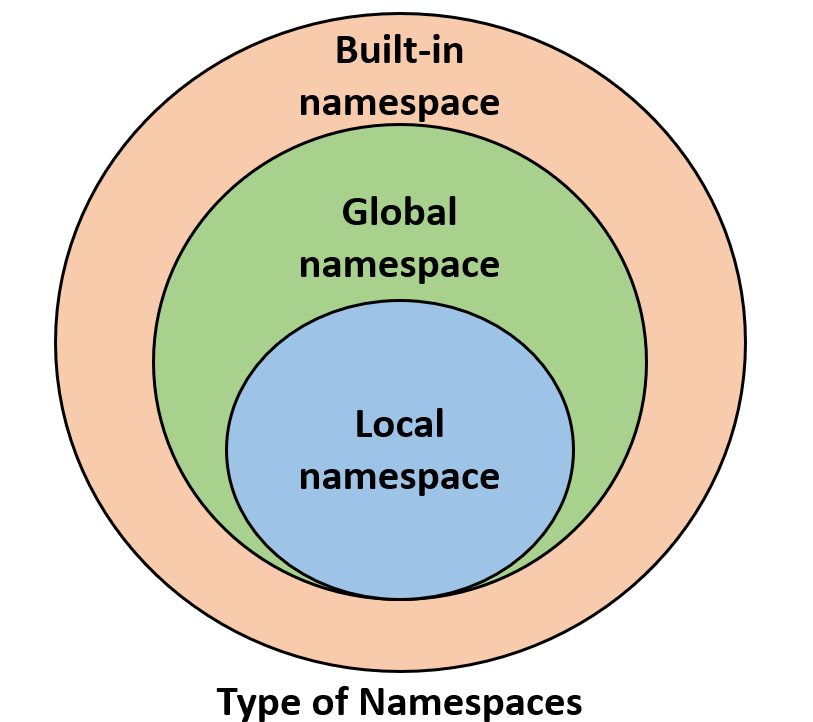
\includegraphics[width=0.25\textwidth]{lez4/namespaces.png}
\end{center}



Python creates separate namespaces for many things: for example, each time a function is called a namespace for local variables is created.\\
You can access objects in the local namespace (and those above -- see picture) just with their name(s); for others you need the '.' (dot) operator.\\

The space of visibility of a variable is called it \alert{scope}.
\subsection{Instance attributes vs class attributes}

  \begin{itemize}
    \small
    \item Each class has a namespace. Plus, each instance of the class get its own additional namespace
    \medskip
    \item The class namespace is automatically visible from each instance namespace, but not the opposite
    \medskip
    \item An attribute in an instance namesespace is an \alert{instance attribute}, and cannot be seen or modified
          by other instances of the class
    \medskip
    \item An attribute in the class namespace is a \alert{class attribute} and is shared among all the instances
    \medskip
    \item Since class attributes are not related to a specific instance, they can be accessed without creating one!
    \medskip
    \item Class attributes are useful to set class constants, or default values, or share data among instances 
  \end{itemize}
  

%Instance attributes: gli elementi della lista hanno ognuno un proprio namespace. 

\subsection{Class attributes (and their strange behaviour)}


\inputminted{python}{snippets/class_attributes_3.py}

\begin{minted}{bash}
[Output]
999
999
998
998
\end{minted}

\hfill
\vfill

\begin{tcolorbox}[width=\textwidth,colback={white},title={Ricapitolando: },colbacktitle=cyan,coltitle=black]
  \begin{itemize}
    \footnotesize
    \item Object Oriented Programming (OOP) is a widespread programming paradigm,
          supported by many programming languages (old and modern), including Python
    \medskip
    \item An object has a state and a behaviour, represented by member variables (attributes)
          and member functions (methods) respectively
    \medskip
    \item A class is a blueprint for creating objects, each object is an instance of a class
    \medskip
    \item In Python classes are defined with the 'class' keyword and instanciated with the '()' operator
    \medskip
    \item Class attributes and methods (globally called members) are accessed through the '.' operator
    \medskip
    \item All the class methods get the object instance as their first argument (usually named 'self')
    \medskip
    \item You should declare class attributes in the constructor a.k.a. the \emph{\_\_init\_\_} function
    \medskip
    \item Instance attributes are not shared: each instance has its own copy of the data
    \medskip
    \item Class attributes are declared outside methods and are shared among all the instances of a class
  \end{itemize} 
\end{tcolorbox}

\newpage


\subsection{Encapsulation - hidden state and interfaces}

C'è un'importante differenza tra interfaccia e implementazione.\\
Pensiamo sempre all'esempio della televisione:




\begin{itemize}
  \item Note that part of the state is hidden from the user (E.g. internal switches, transistors, etc\dots)

  \smallskip
  \item You do not need to know what's going on inside the case to operate a TV!
  \smallskip
  \item All you need to know is how to use the \alert{interface} (the remote
        control, the knobs, the power button, the plug\dots)
  \smallskip
  \item The \alert{implementation} details are hidden: only the TV producer cares about
        them, not the user. 
  \end{itemize}

% Lo stato di un oggetto deve essere modificato   
\begin{itemize}
    \item This leads us to the concept of \alert{encapsulation} 
    \begin{itemize}
      \item \emph{The state of an object should only be accessed and altered
                  through its publicly exposed interface}
    \end{itemize}
    \item That way it is easier to find bugs: you know that, if something is wrong
          with an object, the problem lays inside the class code
    \item That way you can also \emph{enforce behaviour}: for example you can
          prevent from changing the channel if the TV is off
    
\end{itemize}

\textbf{Nota:} una variabile privata è accessibile solo dall'interno della classe.\\

\subsection{Enforcing behaviour}

\inputminted{python}{snippets/class_tv_zapping.py}

\begin{minted}{bash}
[Output]
1
Turning on!
2
\end{minted}

At this point you may be wondering: I can read and modify any class attribute from outside the class using the ’.’ (dot) operator!
Doesn’t that break encapsulation?
Yes it does - but there are ways to fix it!

\subsection{Pythonic encapsulation}


  \begin{itemize}
    \item In languages like C++ you can explicitly declare that some class
          attributes (and methods) are \emph{private}
    \smallskip
    \item In Python there is no concept of \emph{enforced} private attributes
    \smallskip
    \item However, there exists a convention that any attribute/method name prepended by one or two underscore(s) should be considered "private"
    \smallskip
    \item It's like a warning for the class user: you should never access that directly!
    \smallskip
    \item In the case of two underscores Python will actually do a subtle thing to help keeping the data private -- it will 
          prepend \_\emph{classname} to the actual attribute name (see next example)
    \smallskip
    \item However, not everyone in the Python community loves that
    \smallskip
    \item "Never, ever use two leading underscore. This is annoyngly private"\\
           \vspace{0.02\textheight}
           \footnotesize [\emph{Alex Martelli}, member of the Python Software Foundation, author of 'Python in a Nutshell' and co-author of 'The Python cookbook']
  \end{itemize}
  
\subsection{"Private" attributes in Python}

\inputminted{python}{snippets/class_tv_private.py}

\begin{minted}{bash}
[Output]
Sv32X-553T
Alberto
\end{minted}

\subsection{Pythonic encapsulation with properties}

  \begin{itemize}
    \item The possibility of making variables "private" (enforced or not) is not enough of course,
          because sometimes we still want to let the user read or even modify the value of the attribute
    \item The "old" solution for that is providing access functions (the infamous "getters/setters")
    \item But the awsome solution is using \alert{properties} (since Python 2.2)
    \item Properties look similar to getters and setters, but with a twist: you keep
          accessing the attribute with the dot operator
    \item In order to understand why this makes a \emph{huge} difference let's 
          start with an example: suppose you have a class for 2-D vectors
  \end{itemize}

\inputminted{python}{snippets/vector2d_xy.py}

\begin{minted}{bash}
[Output]
3.0 -1.0
3.1622776601683795 -0.3217505543966422
\end{minted}

\begin{itemize}
    \item Suppose you later realize that you use your Vector2d a lot for performing rotations
    \item It would be much faster to store the angle and the module, instead of x and y,
          as the rotation would reduce to a simple addition of the angles
    \item You may think of rewriting your class in that way\dots
  \end{itemize}

\inputminted{python}{snippets/vector2d_rtheta.py}
\noindent In questo caso \texttt{module} e \texttt{angle} sono attributi, mentre \texttt{x} e \texttt{y} sono funzioni.
\begin{minted}{bash}
[Output]
3.1622776601683795 -0.3217505543966422
3.0 -1.0
\end{minted}

  \begin{itemize}
    \item \dots now, however, you have a big problem: your old code is broken!
    \item In every place where your were calling \emph{v.x} or \emph{v.module()}
          now you get an error that needs to be fixed
    \item If other people use your code that is even worse, because you are breaking \emph{their} code
    \item Without properties the solution would have been to design the class from
          the start with private attributes and access functions
  \end{itemize}

\subsection{Old-style encapsulation: never do that!}


\inputminted{python}{snippets/vector2d_old_enc.py}

\begin{minted}{bash}
[Output]
3.0 -1.0
3.1622776601683795 -0.3217505543966422
\end{minted}
  \begin{itemize}
    \item The class data are now "encapsulated", but that is still not ideal:
    \begin{enumerate}
    \item You have written a lot of code just to provide access to a bunch of
          variables
    \item You will have to write even more methods if you want to let the user
          modify that variables as well (e.g. \emph{set\_x(), set\_y()} and so on)
    \item You have to write all this code right from the start, even if you 
          never need it, otherwise you run the risk of getting screwed later
    \end{enumerate}
    \item \alert{properties} solve the problem by \emph{emulating attributes}
  \end{itemize}

\subsection{Properties to emulate attributes}
La property emula l'esistenza di un attributo.

\inputminted{python}{snippets/vector2d_property.py}

\begin{minted}{bash}
[Output]
3.1622776601683795 -0.3217505543966422
3.0 -1.0
\end{minted}

\subsection{Setter properties}

\inputminted{python}{snippets/vector2d_property_setter.py}
Alla riga 25, dietro le quinte sto chiamando il setter (x è un attributo emulato).
\begin{minted}{bash}
[Output]
3.0
1.0000000000000002
\end{minted}

\subsection{Make attributes read-only using properties}


\inputminted{python}{snippets/class_tv_encapsulation_properties.py}

\begin{minted}{bash}
[Output]
This tv belongs to Batman
Nope Joker. Do you want to steal my tv?
This tv belongs to Batman
\end{minted}

\hfill
\vfill

\begin{tcolorbox}[width=\textwidth,colback={white},title={Final note on properties },colbacktitle=cyan,coltitle=black]
  \begin{itemize}
    \item Bottom line: when writing a class, you don't need to make attributes
          private right from the start
    \item You can start with public attributes, and use properties later to
          enforce access/modification rules
    \item That way you only write the code that you really need
  \end{itemize}

Ricapitolando: property permette di fingere che esistano attributi che in realtà non esistono.\\
Inizio con variabili pubbliche. Se in futuro decido di trasformarle in private, definisco una property.\\

Quando scriviamo una classe partiamo con tutte le variabili pubbliche. Dopodiché, se ci accorgiamo ad esempio che una variabile sia di sola lettura: la rendo privata, definisco la property di lettura e poi, volendo, definisco la property di scrittura in modo che mi restituisca un errore.\\
\end{tcolorbox}


\subsection{Interfaccia vs Implementazione}

Quando scriviamo un codice dobbiamo pensarlo in termini dell'interfaccia. \\ L'interfaccia pubblica deve essere più stabile possibile: scrivo il codice in modo da non cambiare l'interfaccia. Nel caso di una classe, gli attributi pubblici fanno parte dell'interfaccia.\\

  \begin{itemize}
    
    \item A physicist thinks:
        
    \medskip
      
    \begin{itemize}
      \item "I have this super-cool algorithm to solve the problem I am working on:
             I will code it carefully, than put together quickly some basic 
             interface to pass data to it and write results to screen / file.
             I need the results quickly for my paper; I can always improve the 
             interface later, right?"
    \end{itemize}
    \medskip
      
    \item A programmer thinks:
    
    \medskip
    
    \begin{itemize}
      \item "I will create a nice interface for the user to handle input/output
             in different formats and I will try to keep it as stable as 
             possible in the future.
             I will start with no algorithm at all -- I will just use random
             numbers to test the interface. I can always implement the
             actual algorithm later, right?"
    \end{itemize}

  \end{itemize}
    
  \begin{itemize}
    \item You don't need to think like a programmer - doing physics is your goal - but
          remember that \alert{interfaces are important}
    \item The concept of interface does not just apply to the program as a whole:
          every significant portion of code (function, class) has its interface
    \item The interface of a class in Python is made by all its "public" members (methods and attributes)
          -- i.e. those without an underscore at the beginning of their name
    \item Changing the interface may break every other piece of code that uses it.
          You want to do that \emph{as less as possible}
    \item You should not access "private" members directly - even if you can. Always
          pass through the interface
    
  \end{itemize}

\hfill
\vfill

\begin{tcolorbox}[width=\textwidth,colback={white},title={Short summary },colbacktitle=cyan,coltitle=black]
  \begin{itemize}
    \small
    \item Encapsulation is the technique of hiding part or all the class state to the user; 
          he can only access and modify that through the class methods
    \medskip
    \item Encapsulation helps debugging by limiting the number of places in the code
          that can mutate the state of an object
    \medskip
    \item It can also be useful to enforce behaviour  
    \medskip
    \item Encapsulation in Python is not enforced by the language, but rather relies on conventions
    \medskip
    \item Class members with an underscore at the beginning of their name are
          considered 'private' and should not be accessed directly oustide the class
    \smallskip
    \item You can use properties to encapsulate your data at any moment in time - never use 'getters' and 'setters'
    \medskip
    \item Interfaces should not change frequently!
  \end{itemize}

\end{tcolorbox}

\newpage

\subsection{Ereditarietà}
L'idea dell'ereditarietà è quella di riutilizzare il più possibile il codice. Funziona creando funzioni specializzate di una classe di partenza.\\
\textbf{Nota:} l'ereditarietà è transitiva.\\

  \begin{itemize}
    \small
    \item Suppose for a moment that you are coding the Monte Carlo for a physics experiment
    \item You want to simulate interactions of charged particles in some detector using OOP paradigm
    \item You may have a class Detetctor and a class for each particle that you need to simulate
    \item Let's say you have a class Electron, a class Positron, a class Proton and a class Alpha
    \item If you think about it, these classes will have a lot of code in common
    \item For example they all need to store their mass, charge, position, velocitiy (or momentum), possibly spin etc\dots
    \item They may also have similar behaviour, though that is less obvious
    \item We know that duplicate code is evil (DRY): how do we avoid that?
  \end{itemize}

  \begin{itemize}
    \small
    \item Many languages - including Python offer a solution for that: \alert{inheritance}
    \item A class can inherit from another one, automatically obtaining all its functionalities (attributes and methods) and then extending or specialyzing them
    \item The class which we inherit from is called \emph{Base} class, \emph{Parent} class or (in Python) \emph{Superclass}
    \item The class inheriting is called \emph{Derived} class or \emph{Child} class
    \item In our problem we can imagine to have a base class 'Particle' and many specialized classes inheriting from it
    \item Inheritance is transtive: if class C inherits from class B, and class B inherits from class A, then class C is also a child of class A (and posses all its functionalities)
  \end{itemize}

\subsection{Inheritance: a basic example}
Nel costruttore della classe figlia si chiama il costruttore della classe madre esplicitamente. Nota: questa chiamata è un po' diversa.\\
\inputminted{python}{snippets/inheritance.py}

\begin{minted}{bash}
[Output]
Energy of e- is 1.1230 MeV/c^2
\end{minted}


\subsection{Overload}
Overload dei metodi: lo stesso metodo lo definiamo sia nella classe madre che nelle classi figlie. Facendo ciò, succede che il metodo nella classe figlia "sovrascrive" il metodo nella classe base.

\inputminted{python}{snippets/overload.py}

\begin{minted}{bash}
[Output]
None
Meow!
Woof!
None
\end{minted}


\subsection{Ereditarietà multipla}

\inputminted{python}{snippets/multiple_inheritance.py}
mro sta per \textit{resolution order}: la classe da cui eredito per prima è la prima in questo ordine di precedenza.

\begin{minted}{bash}
You are listening to channel n. 5
You are looking to channel n. 5
You are listening to channel n. 5
\end{minted}

\textbf{Nota:}Don’t abuse inheritance!\\
In generale: più i pezzi di codice sono indipendenti  e più è facile programmare.

\subsection{Composizione}
Ho come attributo di una classe un oggetto di un'altra classe.\\

  \begin{itemize}
    \item \alert{Composition} is a different technique for reusing functionalities
    \item The concept is simple: just use an object of some class as a member of
          a different one
    \item For example we can create the classes 'Enigne' and 'Wheel' and than 
          the class 'Car' will have a member of type Engine and 4 members of
          type Wheel
    \item A class like 'Car' in the example is sometimes called an 
          \alert{aggregate} class
  \end{itemize}

\inputminted{python}{snippets/composition.py}


\begin{minted}{bash}
[Output]
Broom broom!
\end{minted}


\subsection{Composition vs Inheritance}

la composizione si usa quando voglio rappresentare una classe di appartenenza. Mentre con l'ereditarietà rappresento una relazione diversa: un elettrone eredita dalla classe particella perché un elettrone è una particella.\\
  \begin{itemize}
    \item Composition models a \alert{'has-a'} relation in the real world: a 
          Car \emph{has} a Engine
    \item Inheritance models a \alert{'is-a'} relation in the real world: an
          Electron \emph{is} a Particle
    \item It may not always be obvious which one to use in your specific case:
          choose wisely!
  \end{itemize}
  
Se siamo nel dubbio è meglio usare la composizione: è più safe.


\subsection{Pitfalls of Inheritance}
  \begin{itemize}
    \item Inheritance is a wild beast. There are entire libraries written about how and when (not) to use it
    
    \bigskip
    
    \item Question for you: should a Square inherits from a Rectangle?
    \item Seems legit: a Square \emph{is} a specialized Rectangle
    \item But what happens if the Rectangle class has a changeHeight() method?
    \bigskip
    
    \bigskip
    
    \item \alert{Liskov Substitution Principle}: you should always be able to use
          a derived class instead of a base class in your code
    \item In other words: a derived class should always extend or specialize
          the functionalities of the base class, never restrict them!
   \end{itemize}
   
\hfill
\vfill
  

\begin{tcolorbox}[width=\textwidth,colback={white},title={Short summary },colbacktitle=cyan,coltitle=black]
  \begin{itemize}
    \item A class can inherit funcionalities from one or more other classes (Inheritance)
    \medskip
    \item The class that inherits is call Derived (or Child) class the inherited one is the Base (or Parent) class
    \medskip
    \item Inheritance models an \emph{is-a} relationship
    \medskip
    \item Classes can also incorporate other objects as class members (Composition)
    \medskip
    \item Composition models an \emph{has-a} relationship
    \medskip
    \item Inheritance is tricky: use it with care!
   \end{itemize}

\end{tcolorbox}

\newpage
\section{\textit{Gio 6 ott - Lezione 5}}

\section{Lecture basic: 5 - OOP Introduction (2/2)}

  \begin{itemize}
    \item Suppose we want to create a class for managing 2D vectors\footnote{%
      The content of this lesson is vastly based on the the book '\emph{Fluent Python}' by Luciano Ramalho}
    \item That's just for learning: there are already plenty of libraries for
          doing array operations - like numpy!
    \item Anyway let's start coding some useful methods for it
  \end{itemize}
  

\inputminted{python}{snippets/vector2d_naive.py}
\begin{minted}{bash}
[Output]
Vector2d(3.0, -1.0)
3.1622776601683795
Vector2d(4.0, 0.5)
\end{minted}

  \begin{itemize}
    \item This kind of works but\dots... isn't that ugly?
    \item Look at the lines \emph{v.info()} or \emph{v.module().}
          It would be far more readible to just do \emph{print(v)} and \emph{abs(v)}
    \item And what about \emph{t = v.add(z)}? Why not \emph{t = v + z}?
    \item In Python there is a tool that allows you to do just that: \alert{special methods}
    \item Last lesson we saw that special methods (or dunder methods or 
          magic methods) are methods like \emph{\_\_init\_\_} and got a special
          treatment by the Python interpeter
    \item There are a few tens of special methods in Python. Let's see how they work
  \end{itemize}

\subsection{Special Methods}


\inputminted{python}{snippets/vector2d_2.py}
\begin{minted}{bash}
[Output]
3.1622776601683795
\end{minted}

  \begin{itemize}
    \item And what about \emph{print()}?
    \item There are actually two special methods used for that: \emph{\_\_str\_\_} and \emph{\_\_repr\_\_}
    \item \emph{\_\_str\_\_} is meant to return a concise string for the user; it is called with \emph{str()}
    \item \emph{\_\_repr\_\_} is meant to return a richer output for debug. It is called with \emph{repr()}
    \item \emph{print()} automatically tries to get a string out of the object using \emph{\_\_str\_\_}
    \item If there isn't one, it searches for \emph{\_\_repr\_\_}. A defealut \emph{\_\_repr\_\_}
          is automatically generated for you, if you haven't defined one
  \end{itemize}

\subsection{\emph{\_\_str\_\_} and \emph{\_\_repr\_\_}}

\inputminted{python}{snippets/vector2d_printable.py}
\begin{minted}{bash}
[Output]
(3.0, -1.0)
Vector2d(3.0, -1.0)
I got (3.0, -1.0) with __str__ and Vector2d(3.0, -1.0) with __repr__
\end{minted}

\subsection{Mathematical operations}

\inputminted{python}{snippets/vector2d_math.py}
\begin{minted}{bash}
[Output]
(-2.0, 0.0)
(9.0, -3.0)
(-25.0, 5.0)
\end{minted}

\subsection{In-place operations}
\inputminted{python}{snippets/vector2d_inplace.py}
\begin{minted}{bash}
[Output]
(-2.0, 0.0)
(10.0, 0.0)
\end{minted}

L'addizione fatta con \texttt{\_\_iadd\_\_} è concettualmente diversa da quella fatta con \texttt{\_\_add\_\_}. Infatti in questo caso non sto creando un nuovo vettore, ma sto modificando gli attributi del vettore su cui è chiamata la funzione.

\subsection{Comparisons}

\subsection{In-place operations}
\inputminted{python}{snippets/vector2d_comparable.py}
Alla riga 15 sfruttiamo l'uguaglianza delle \textit{tuple} in modo da risparmiarci l'implementazione from scratch dell'uguaglianza tra float.
\inputminted{python}{snippets/test_vector2d_comparable.py}
\begin{minted}{bash}
[Output]
True False False
False
[Vector2d(3.0, -1.0), Vector2d(-5.0, 1.0), Vector2d(3.0, 0.0)]
[Vector2d(3.0, 0.0), Vector2d(3.0, -1.0), Vector2d(-5.0, 1.0)]
\end{minted}


\subsection{An hashable Vector2d}
  \begin{itemize}
    \item Ok now let's try to make our vector2d \emph{hashable}
    \item Hashable objects can be put in \emph{sets} and used as keys for 
          dictionaries
    \item To make an object hashable we need to fullfill 3 requirements:
    \begin{itemize}
      \item It has to be immutable - otherwise you may not retrieve the correct hash
      \item It needs to implement a \emph{\_\_eq\_\_} function, so one can compare
            objects of this class
      \item It needs a (reasonable) \emph{\_\_hash\_\_} function
    \end{itemize}
    \item Rules for a good hash function:
    \begin{itemize}
      \item Must return the same value for objects that compare as equal
      \item Should rarely return the same value for different objects
      \item Should sample the result space uniformly
    \end{itemize}
    
  \end{itemize}


\inputminted{python}{snippets/vector2d_hashable.py}

\inputminted{python}{snippets/vector2d_hashable_test.py}

\begin{minted}{bash}
[Output]
False True False
-3 -6 -3
Vector2d(-5.0, 1.0), Vector2d(3.0, -1.0)
Vector2d(3.0, -1.0)
\end{minted}

\subsection{Array N-dimensionali}

  \begin{itemize}
    \item 2d array are boring\dots why not a N-d array?
    \item Of course we cannot store the components explicitly like before
    \item We need a container for that and we will use \emph{array} from the 
          array library
    \item This is an example of \alert{composition}
   
    \item Question for you: why not a list or a tuple? $\rightarrow$ Perché le liste sono lente, non sono pensate per fare operazioni matematiche (i dati in memoria non sono contigui) 
    \item Note: \emph{array} uses a typecode (a single character) for picking the
          type. 'd' is the typecode for float numbers in double precision. 
  \end{itemize}
  
  
\inputminted{python}{snippets/vector.py}
A riga 6 stiamo salvando il \texttt{typecode} come attributo della classe: ovvero è condiviso con tutte le istanze della classe.
\begin{minted}{bash}
(5.0, 3.0, -1.0, 8.0)
Vector([5.0, 3.0, -1.0, 8.0])
\end{minted}

  \begin{itemize}
    \item Now that we have an arbitrary number of components, we cannot access them like 
          vector.x, vector.y, \dots anymore
    \item What we want is a syntax similar to that of lists: vector[0], vector[1]
          ans so on
    \item There are two magic methods for that: \emph{\_\_getitem\_\_} for access 
          and \emph{\_\_setitem\_\_} for modifying
    \item While we are at it, we also implement the \emph{\_\_len\_\_} method,
          which allows us to call \emph{len(vector)}
  \end{itemize}
  
\inputminted{python}{snippets/vector_random_access.py}

\inputminted{python}{snippets/test_vector_random_access.py}

\begin{minted}{bash}
[Output]
4
5.0 3.0
Vector([5.0, 10.0, -1.0, 8.0])
Traceback (most recent call last):
    File "snippets/test_vector_random_access.py", line 12, in <module>
        print (v[9]) # This will generate an error!
    File "/data/work/teaching/cmepda/slides/latex/snippets/vector_random_access.py", line 13,
        return self._components[index]
IndexError: array index out of range
\end{minted}  

\subsection{An Iterable Vector}

  \begin{itemize}
    \item Now our vector behaves a bit like a native python list
    \item However a list has a very powerful feature we miss: it's \alert{iterable}
    \item An \emph{iterable} in Python is something that has a
          \emph{\_\_iter\_\_} method, which returns an \alert{iterator}
    \item Technically, an iterator is an object that implements the
          \emph{\_\_next\_\_} special method, which is used to retrieve elements
          one at a time
    \item We will not dicuss iterators any further here: instead, we will just
          exploit composition and borrow the \emph{\_\_iter\_\_} method from the 
          underlying array
  \end{itemize}

\inputminted{python}{snippets/vector_iterable.py}
\begin{minted}{bash}
[Output]
5.1
3.7
-25.0
\end{minted} 

\subsection{Duck Typing\footnote{"If it looks like a duck and quacks like a duck, it must be a duck."}}


\inputminted{python}{snippets/duck_typing.py}

\begin{minted}{bash}
[Output]
Quack!
Quack!
Traceback (most recent call last):
    File "snippets/duck_typing.py", line 20, in <module>
        bird.quack()
AttributeError: ’Penguin’ object has no attribute ’quack’
\end{minted} 


\subsection{Polymorphism}
  
  \begin{itemize}
    \item Reuse the same code for different things
    \item In statically typed languages this is tipically done with inheritance,
          e.g. we make Duck and Goose inherits from a base class QuackingBird()
          or something like that
    \item Python is dynamical, so we can use duck typing for that.
          We just need to implment the quack() method for both Ducks() and Goose() 
          and we are done
    \item In other words we obtain polymorphism just by satsisfying the required \alert{interface}
          (in this case the quack() function)
  \end{itemize}
  
  \subsection{The power of iterables}
  \begin{itemize}
    \item Having an iterable Vector (thanks to the \emph{\_\_iter\_\_} magic
          method) makes all the difference in the world
    \item There are \emph{a lot} of builtin and library functions in python accepting a
          generic iterable as input:
    \begin{itemize}
      \item \emph{sum}: Sum all the elements
      \item \emph{max}/\emph{min}: Return the maximum/minimum
      \item \emph{enumerate}: Iterate with automatic counting of iterations
      \item \emph{map}: Apply a function to the elements one by one
      \item \emph{filter}: Iterate only on the elements passing a given condition
      \item \emph{zip}: Iterate over pairs of elements (requires two iterables)
    \end{itemize}
    \item Countless others can be found in the \alert{\emph{itertools}} library
    \begin{itemize}
      \item \emph{islice}: Slice the loop with start, stop and step
      \item \emph{takewhile}: Stop looping when a condition becomes false
      \item \emph{chain}: Loop through many sequences one after another
      \item \emph{cycle}: Loop over the sequence repeatedly, indefinitely
      \item \emph{permutations}: Get all the permutations of a given length
      \item And so on\dots
    \end{itemize}
    \item With duck typing we can now use any of that for our Vector class -- isn't that cool?
  \end{itemize}

\inputminted{python}{snippets/vector_iterable_test.py}

\begin{minted}{bash}
[Output]
[4.0]
(1.0, 2.0)
(1.0, 4.0)
(2.0, 1.0)
(2.0, 4.0)
(4.0, 1.0)
(4.0, 2.0)
\end{minted} 

\subsection{A vector that behaves like a duck}
\inputminted{python}{snippets/vector_ducked.py}
\inputminted{python}{snippets/test_vector_ducked.py}
\begin{minted}{bash}
[Output]
(1.0, 2.0, 3.0)
3.741657386773941
6.0
False False True
(2.0, 4.0, 8.0)
(2.0, 4.0, 6.0)
\end{minted} 

\subsection{Function are classes}
  
  \begin{itemize}
    \item Remember that in the past lesson I told you that functions are objects
          of the 'function' class.
    \item How are they implemented?
    \medskip
    \item With a special method - of course: \emph{\_\_call\_\_}
    \item Every object implementing a \emph{\_\_call\_\_} method is called \alert{callable}
  \end{itemize}
  
Esempio: Noi tipicamente a \texttt{curve\_fit} passiamo una funzione, ma in realtà possiamo passarle un qualsiasi \textit{callable}!

\subsection{A simple callable for a straight line}

\inputminted{python}{snippets/callable_line.py}
\begin{minted}{bash}
[Output]
y = -2.0 x + 1.0
Slope = -2.0, Intercept = 1.0
-3.0
\end{minted} 

\subsection{Create a call counter}

\inputminted{python}{snippets/callable.py}
Il \textit{"wrapper"} aggiunge un layer di funzionalità intermedie.\\
Riga 16: siccome non conosciamo quali argomenti prende questa funzione, dobbiamo fare in modo che prenda un qualsiasi numero di argomenti.\\

\subsection{Fit hacking}

\inputminted{python}{snippets/test_callable.py}
Riga 15: sto passando a \texttt{curve\_fit} la funzione \textit{"wrappata"}. In questo caso devo per forza passargli p0, altrimenti \texttt{curve\_fit} non ha modo di capire il numero di parametri: tipicamente per capirlo guarda gli argomenti della funzione che gli passiamo, ma in questo caso gli stiamo passando un callable generico!
\begin{minted}{bash}
[Output]
Fitted with 9 function calls
\end{minted} 

\begin{figure}[ht]
    \centering
    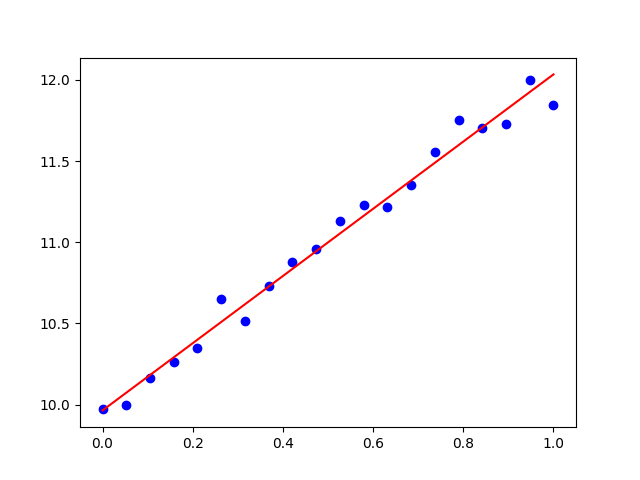
\includegraphics[width=0.6\textwidth]{lez5/fit.png}
    \caption{The fit works as usual}
    \label{fit}
\end{figure}
\FloatBarrier

\vfill
\hfill

\begin{tcolorbox}[width=\textwidth,colback={white},title={Summary: },colbacktitle=cyan,coltitle=black]
  \begin{itemize}
    \item Special methods can beused to greatly enhance the readibility of the code
    \item There are tens of special methods in python, covering logical operations,
          mathematical operations, array-style access, iterations, formatting and
          many other things\dots
    \item Implementing the required interface in your classes you will be able
          to reuse a lot of code written for the standard containers thanks to
          duck typing, which is the pythonic way to polymorphism
   \end{itemize}  
\end{tcolorbox}

\newpage

\section{\textit{Lun 10 ott - Lezione 6}}

\section{Lecture Advanced 1: Testing and documentation}

\subsection{How do I make sure my program is correct?}
In un linguaggio compilato alcune le verifiche le fa il compilatore, che fa per lo meno alcune verifiche. Nei linguaggi interpretati, come python è più difficile, perché fino a quando non \textbf{eseguiamo} il codice, nessuno sa che argomenti passiamo a una funzione.
Si fanno due cose nei linguaggi interpretati: unit testing e static analysis (es. pylint).

  \begin{itemize}
  \item The short answer is: in real life you don't!
    \begin{itemize}
    \item Especially if your code is asynchronous
    \end{itemize}
  \item \alert{That is not the same a saying there is nothing you can do}
  \item For compiled langauges the compiler will flag all obvious (and a whola
    lotta of non-obvious) mistakes
    \begin{itemize}
    \item This doesn't really apply to Python, since Python is interpreted
    \item Although the interpreter will stop upon syntax errors
    \end{itemize}
  \item Besides paying attention, there are two things that you can do even
    in interpreted languages:
    \begin{enumerate}
    \item \alert{Unit testing}
    \item \alert{Static analysis}
    \end{enumerate}
  \item Generally people hate both, but they should come right next to
    version control in your work-flow toolbox
  \end{itemize}

\subsection{Unit testing na\"ive example}

\inputminted{python}{snippets/unit_test_naive.py}

\begin{minted}{bash}
[Output]
Passed---cool!
\end{minted} 

Il test in questo caso si assicura che il quadrato di 2 faccia 4.
Chiaramente questo è un caso particolare. Unit testing significa spezzare il codice in unità elementari, individuare alcuni casi interessanti e verificare che in questi casi tutto funzioni a dovere.\\
Se facciamo crescere il nostro programma organicamente con una serie di unit test, riusciamo ad evitare molti errori!

\subsection{Unit testing in a nutshell}

  \begin{itemize}
  \item Break up your program in many small pieces
    \begin{itemize}
    \item Each piece should encapsulate a well-defined and (possibly) simple
      functionality. \textit{Le funzioni che fanno 100 cose insieme non vanno bene, è meglio scomporle in 100 funzioni!}
    \end{itemize}
  \item This is usually accomplished by means of a sensible hierarchy of
    functions and classes
    \begin{itemize}
    \item And this is typically the hardest task when structuring your code
    \item And the code will evolve with time, so you will find yourself
      \alert{refactoring code} from time to time
    \item Remember to be dry: don't repeat youself
    \end{itemize}
  \item \alert{Unit testing is: make sure that each single piece is
    correct by implementing a series of basic checks}
    \begin{itemize}
    \item You know what each elementary piece of code is suppose to be
    \item Make sure it does
    \item And make sure it does with any valid input
    \end{itemize}
  \item This is much simpler that testing the whole program at once
    \begin{itemize}
    \item Although you have to do that, too
    \end{itemize}
  \item \alert{Test-Driven Development (TDD)}
    \begin{enumerate}
    \item Write an empty placeholder for your new function
    \item Write all the unit tests (they will fail)
    \item Implement your function and tweak it until all the tests pass
    \end{enumerate}
  \end{itemize}
\textbf{TDD:} Quando scriviamo un codice, tipicamente abbiamo delle specifiche da rispettare. Scrivo prima il test in base alle specifiche; poi scrivo il corpo vuoto della funzione; e infine implemento la funzione finché passi tutti i test.

\textbf{\'E importante scrivere test e documentazione di pari passo con la stesura del codice! Non devo aspettare la fine per farli!}

\subsection{Back to our na\"ive example}

Cosa può andare storto?\\
Cosa succede se passo una stringa alla nostra funzione? Avrò un TypeError. In questo caso è facile individuare l'errore, ma a volte non è così semplice. \'E molto utile scrivere un unit test che controlli che in input alla funzione sto dando un numero.\\
Ci sono infiniti modi in cui una cosa potrebbe andare storto!
\inputminted{python}{snippets/unit_test_naive.py}

\begin{minted}{bash}
[Output]
Passed---cool!
\end{minted} 

  \begin{itemize}    
  \item This is fine, but everything happens manually
    \begin{itemize}
    \item You have to run the script yourself
    \item You have to inspect the output yourself
    \end{itemize}
  \item As your code grows in complexity, this is not very effective
  \end{itemize}

[Le variabili d'ambiante sono la chiave per il funzionamento del sistema operativo.]

\subsection{Unit tests the Python way: The unittest module}

C'è un altra cosa che si chiama pytest, che ultimamente ha soppiantato unittest, ma la logica è la stessa.\\
Idealmente ogni volta che faccio una modifica vorrei runnare tutti i test.\\
C'è una cosa che si chiama \textbf{continous integration}.
\inputminted{python}{snippets/unit_test.py}

\begin{minted}{bash}
[Output]
.
----------------------------------------------------------------------
Ran 1 test in 0.000s
OK
\end{minted} 

\subsection{Wait a moment\ldots How is this different?}

  \begin{itemize}
  \item This is much better!
  \item The base TestCase class offers all the goodies for unit testing
    \begin{itemize}
    \item assertTrue(), assertFalse(), assertEqual(), assertAlmostEqual()\ldots
    \end{itemize}
  \item The execution can be easily made automatic:
    \begin{itemize}
    \item Put all your unit test modules into a test folder
    \item Run \texttt{python -m unittest discover}
    \item (Or, even better, write a small Makefile or .bat script to do that)
    \item That's it---all your tests are run in sequence
    \end{itemize}
  \item Did you just find a bug in your code?
    \begin{itemize}
    \item Make sure you add a unit test along with the fix, so that you'll
      never be hurt again by that particular bug
    \end{itemize}
  \item Are you adding a new feature?
    \begin{itemize}
    \item Make sure the new code is covered by unit tests
    \item You should not be obsessed by the coverage, but you should
      definitely aim for it to be as large as possible
    \end{itemize}
  \item \alert{You should always make sure that all the unit tests are
    passing before merging stuff on the master}    
  \item More about this in a bit (we'll be talking about continuous integration)
  \end{itemize}

\subsection{Static code analysis}

  \begin{itemize}
  \item By its very nature, Python will show you all the errors at runtime
  \item Say you have a bug in a part of the code that is exercised very rarely,
    and not covered by unit tests
    \begin{itemize}
    \item Python might crash the first time you exercise it\ldots
    \item or Python might happily do \emph{something} that is not what you
      intended
    \end{itemize}
  \item \alert{It might take years for even realizing that there is a bug}
  \item Many common mistakes can be found by just looking at the code
    \begin{itemize}
    \item And in fact all of them can, at least in principle
    \end{itemize}
  \item Part of it can be done programmatically
    \begin{itemize}
    \item Generally, a program will not \emph{understand} your program
    \item But a program can be trained to spot some kind of
      errors and inconsistencies
    \end{itemize}
  \item Pylint and pyflakes are good examples of such tools
  \end{itemize}

\subsection{Static analysis: an example}

\inputminted{python}{snippets/linting1.py}

\begin{minted}{bash}
[Output]
3.0
\end{minted} 

  \begin{itemize}
  \item And here is the pylint output
  \end{itemize}
  
  {\scriptsize
    \begin{Verbatim}
[lbaldini@nbbaldini latex]$ pylint snippets/linting1.py 
************* Module snippets.linting1
snippets/linting1.py:1:0: C0111: Missing module docstring (missing-docstring)
snippets/linting1.py:1:0: C0103: Constant name "x" doesn't conform to UPPER_CASE
                          naming style (invalid-name)
snippets/linting1.py:2:0: C0103: Constant name "y" doesn't conform to UPPER_CASE
                          naming style (invalid-name)
snippets/linting1.py:3:0: C0103: Constant name "very_uncommon_condition" doesn't
                          conform to UPPER_CASE naming style (invalid-name)
snippets/linting1.py:5:14: E0602: Undefined variable 'z' (undefined-variable)

--------------------------------------------------------------------
Your code has been rated at -5.00/10 (previous run: -5.00/10, +0.00)
    \end{Verbatim}
  }
  
\subsection{Static code analysis}  

  \begin{itemize}
  \item \alert{You should consider using static code analysis routinely}
  \item Static analysis tools tend to be quite verbose
    \begin{itemize}
    \item And often times verbose is the same as annoying
    \end{itemize}
  \item They try and enforce many different (good!) things at once
    \begin{itemize}
    \item Formal correctness
    \item Efficiency
    \item Avoiding anti-patterns
    \item Style guides
    \item Generic conventions
    \end{itemize}
  \item They also are typically highly customizable
    \begin{itemize}
    \item i.e., you can mute errors you don't care about
    \item But be advised: you most of the times you should probably care
    \end{itemize}
  \item \alert{Finding a good balance is generally not too hard}
  \item And trust me: it will help you in the long run
  \end{itemize}

\subsection{Digression: optional static typing in Python}

\inputminted{python}{snippets/type_annotation.py}

\begin{minted}{bash}
[Output]
4.0
4.0
\end{minted} 

  \begin{itemize}
  \item Recent Python 3 versions support type annotations
  \item \alert{The Python interpreter recognizes but does nothing with
    annotations}
    \begin{itemize}
    \item And so what?
    \end{itemize}
  \item Well\ldots they are handy (as comments are)
    \begin{itemize}
    \item The code is easier to read
    \item Even more checks wrt un-annotated code can be done by tools such as
      mypy
    \end{itemize}
  \end{itemize}

\subsection{Continuous integration}

  \begin{itemize}
  \item Imagine for a second\ldots
    \begin{itemize}
    \item Wouldn't it be nice if sombody run all the unit tests of my
      package every time I push on the master or make a pull request?
    \item And, since we are at it, sent me an email if any of the tests fail?
    \end{itemize}
  \item \ldots Well, such a thing exists and it is standard practice in
    code dvelopment
  \item People even made a name for it: \alert{Continuous Integration (CI)}
  \item CI cloud-base services exists just like code-hostng services exist
    \begin{itemize}
    \item Travis-CI and circleci are two good examples
    \end{itemize}
  \item They interoperates seamlessly with github, gitlab or bitbucket
  \item Setting up CI for your package is usually fairly simple
  \item \alert{One-sentence summary: go ahead and do it. Always.}
  \end{itemize}
  
  
\subsection{Documentation}
La documentazione vive insieme al codice! E il meccanismo che si usa per implementare il codice sono le "docstring". C'è una sintassi ben precisa che permette ad un tool automatico, che nel caso di python si chiama Sphynx, di generare la documentazione.\\

Ci sono vari programmi di host per la documentazione (ad esempio uno open source è \textbf{readthedocs}).


\begin{figure}[ht]
    \centering
    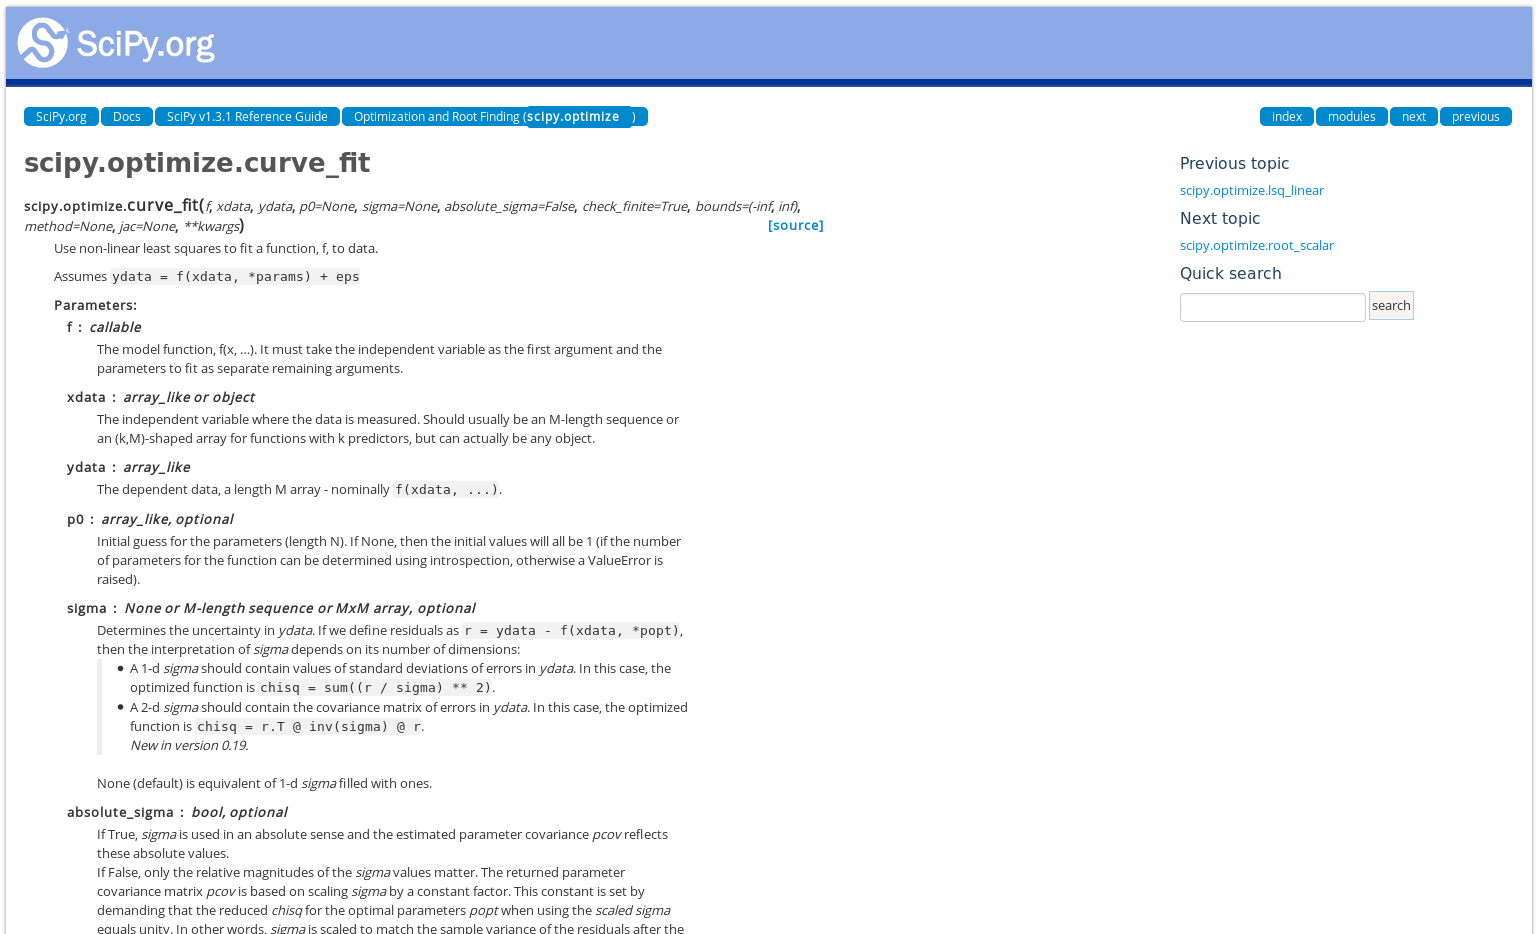
\includegraphics[width=1\textwidth]{lez6/doc_scipy.png}
    \caption{How do the hell they do that?}
    \label{scipy_documentation}
\end{figure}
\FloatBarrier

\begin{figure}[ht]
    \centering
    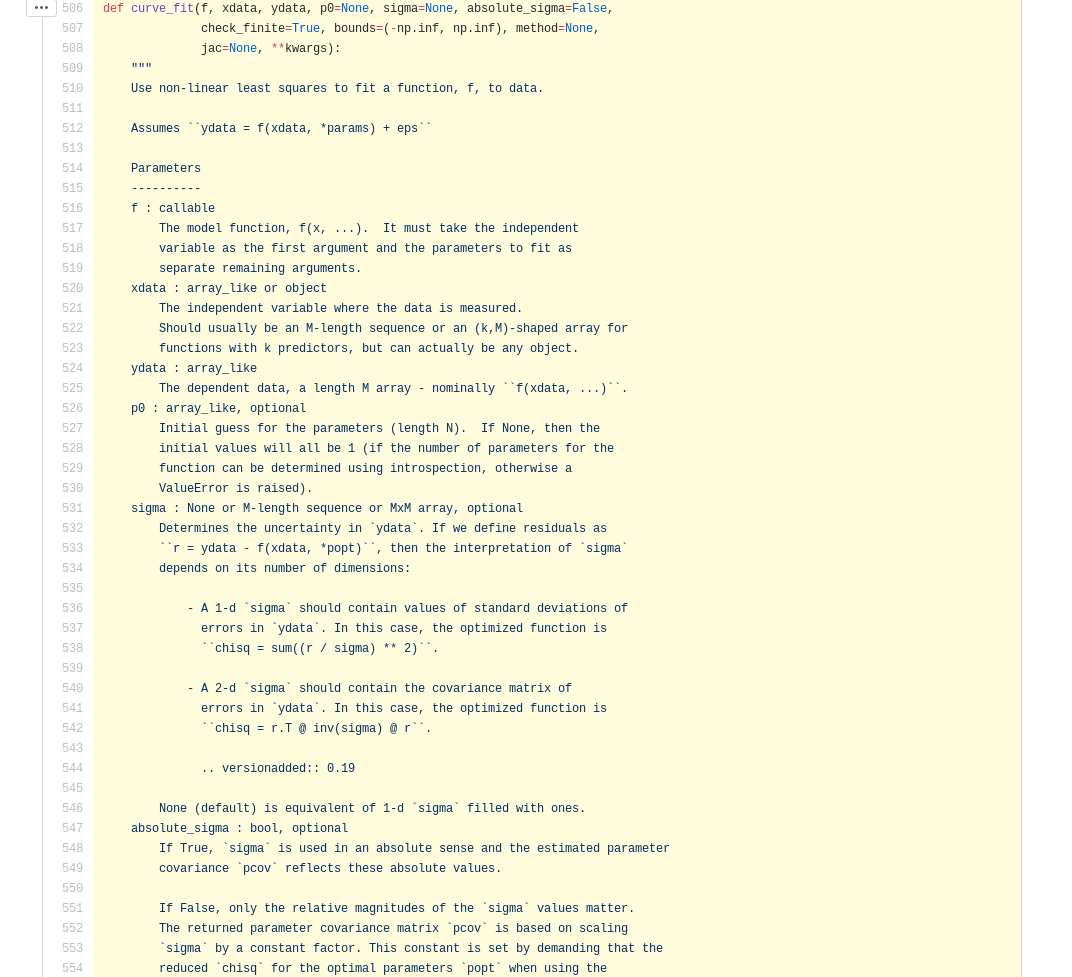
\includegraphics[width=1\textwidth]{lez6/codice_doc.png}
    \caption{the documentation is embedded in the code. . .}
    \label{documentation_code}
\end{figure}
\FloatBarrier

\subsection{Sphinx: the documentation tool for Python}


\subsection{Sphynx basics}

  \begin{itemize}
  \item Process all the relevant information to produce several types of
    output
    \begin{itemize}
    \item Most notably html and LaTeX
    \end{itemize}
  \item Two different sources:
    \begin{enumerate}
    \item The doctrings in the Python modules
    \item Additional markup files (in reStructuredText) containing
      auxiliary information
    \end{enumerate}
  \item Typical workflow:
    \begin{itemize}
    \item Use \texttt{sphinx-quickstart} once when you setup your project
    \item Tweak the generated \texttt{conf.py} file to suit your needs
    \item Go ahead and have fun!
    \end{itemize}
  \item Sphinx is \emph{very} powerful
    \begin{itemize}
    \item e.g., \url{https://docs.python-guide.org/} is written in Sphinx,
      and so is all the Python documentation
    \end{itemize}
  \end{itemize}


\begin{figure}[ht]
    \centering
    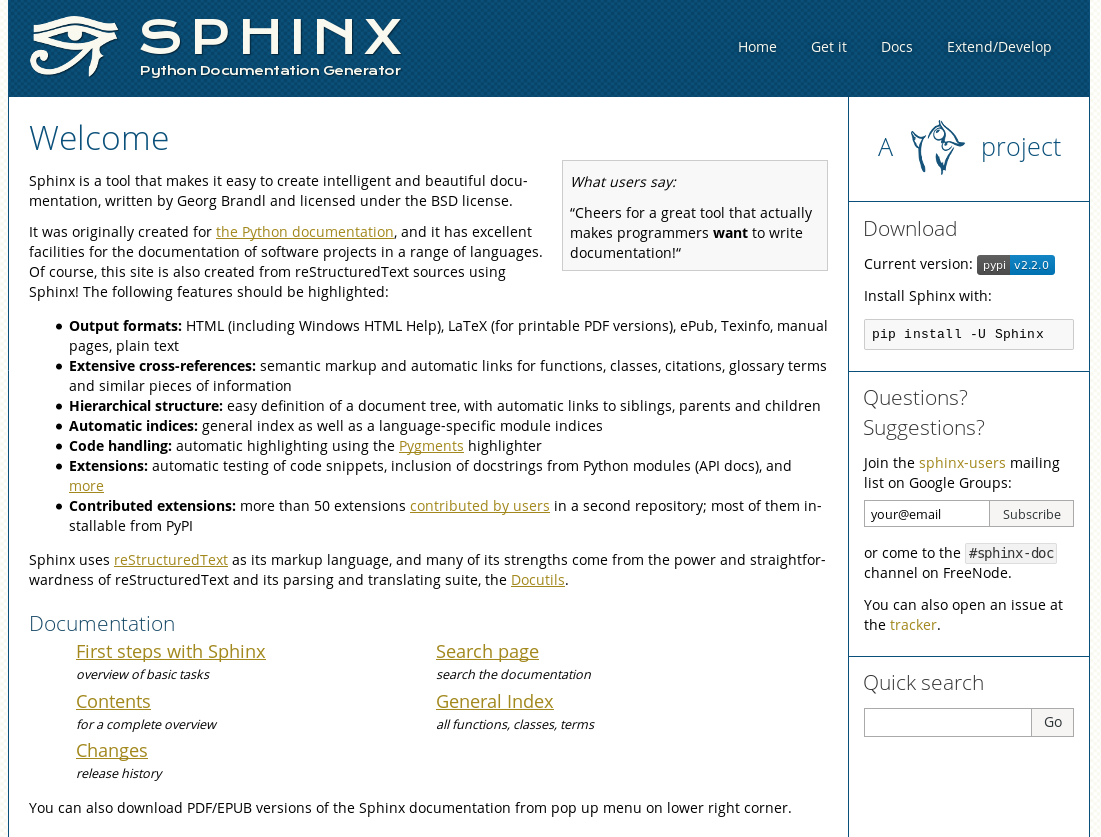
\includegraphics[width=0.9\textwidth]{lez6/sphinx.png}
    \caption{.}
    \label{sphynx}
\end{figure}
\FloatBarrier

\subsection{Ok, I have the documentation compiled, now what do I do with it?}

  \begin{itemize}
  \item Wouldn't it be nice if the documentation was automatically compiled and
    uploaded on the web each time I push on the master?
  \item This is possible and is called readthedocs.com
    \begin{itemize}
    \item And, again, this is a cloud-based service that can interoperate
      easily with github, gitlab or bitbucket
    \end{itemize}
  \end{itemize}


\textbf{NOTA: Per il progetto di fine anno bisogna fare tutto questo, compreso avere la documentazione su un sito come readthedocs}.


\newpage

\section{Torniamo a numpy}
L'ultima volta abbiamo visto il broadcasting.\\

\subsection{Mathematical functions in Numpy}

\inputminted{python}{snippets/numpy_functions.py}

\begin{minted}{bash}
[Output]
[-1. 0. 1.]
[1.10517092e+00 2.71828183e+00 2.20264658e+04]
[ 0.09983342 0.84147098 -0.54402111]
-1.0
Traceback (most recent call last):
    File "snippets/numpy_functions.py", line 12, in <module>
        print(math.log10(a))
TypeError: only size-1 arrays can be converted to Python scalars
\end{minted}

numpy mathematical functions interoperate natively with arrays (and work on plain old numbers, too).

\subsection{Array and Masks}
Masks are a powerful tool in numpy. They can replace conditional expressions in a for loop in vectorization context .

\inputminted{python}{snippets/numpy_masks.py}
\begin{minted}{bash}
[Output]
[ 0. 1. 2. 3. 4. 5. 6. 7. 8. 9. 10.]
[False False False True True True True True True True]
[ True True True True True True True True True False False]
[ 3. 4. 5. 6. 7. 8. 9. 10.]
[0. 1. 2. 3. 4. 5. 6. 7. 8.]
[3. 4. 5. 6. 7. 8.]
\end{minted}

\textbf{Altro esempio:}

\begin{minted}{python}
a = np.random.uniform(size=10)
mask = a > 0.5

mask.sum() #mi restituisce il numero di elementi che soddisano la condizione

#posso passare una maschera tra parentesi quadre per indirizzare gli elementi di un array.
#Mi restituisce un nuovo array contenente solo gli elementi che soddisfano la condizione

a[mask]
\end{minted} 


\textbf{Da fare: guardare come si fa lo slicing di un array}


\subsection{Digression: pseudo-random number generators}

\begin{minted}{python}
import random
x = random.random()
\end{minted}

\begin{itemize}
  \item Every programming language comes with a Pseudo Random Number
    Generator (PRNG)
    \begin{itemize}
    \item Python is no exception:
      \url{https://docs.python.org/3/library/random.html}
    \item Mersenne-Twister, 53-bit precision, period of $2^{19937} - 1$. 
    \end{itemize}
  \item PRNGs are an interesting (and fun) subject by themselves:
    \begin{itemize}
    \item Donald E. Knuth, \emph{The Art of Computer Programming, Volume 2: Seminumerical Algorithms}, 3rd Edition 
    \item M. Matsumoto and T. Nishimura, \emph{Mersenne Twister: A 623-dimensionally equidistributed uniform pseudorandom number generator}, ACM Transactions on Modeling and Computer Simulation Vol. 8, No. 1, January pp.3--30 1998.
    \end{itemize}
  \item A PRNG produces random floats uniformly in $[0.0,~1.0)$.
  \end{itemize}
  
\textbf{Nota} Il modulo random di numpy mi permette di generare numeri random non uno alla volta, ma in array!

\subsection{Vettorizzazione}
Avoid explicit for loops in Python whenever you can!

\textbf{pandas}: utile per leggere e scrivere file excel.

\inputminted{python}{snippets/vectorization.py}
\begin{minted}{bash}
[Output]
Elapsed time: 0.137 s
Elapsed time: 0.015 s
\end{minted}

\subsection{How does vectorizaion work?}


  \begin{itemize}
  \item Python is know to be slooow
    \begin{itemize}
    \item This is the price you pay for being so beautiful and flexible
    \end{itemize}
  \item Does it matter? If depends\ldots
    \begin{itemize}
    \item If you are parsing a text file or fetching a web page probably not
    \item If you are performing a CPU-intensive processing on a TB of data
      probably yes
    \end{itemize}
  \item What's so magic in using numpy?
  \item numpy is written in C as a Python extension
    \begin{itemize}
    \item Routines are highly optimized to cruch numbers
    \item When you perform an array operation in Python you are actually
      executing optimized C code
    \end{itemize}
  \item \alert{Basic message: avoid for loops in pure Python when
    crunching numbers}
  \end{itemize}

\newpage

\section{Secondo Assegnamento}

\subsection{How do I throw PRN with arbitrary pdf?}


\textbf{Hit or miss:}
\begin{center}
  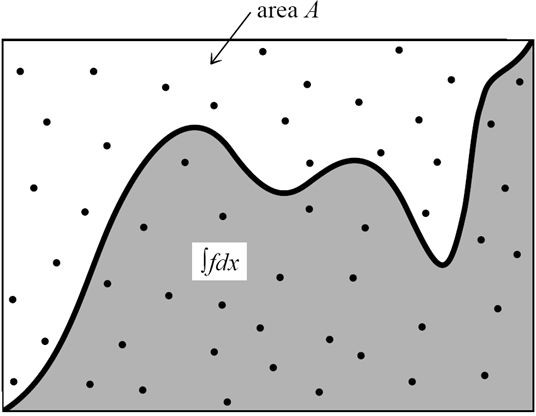
\includegraphics[width=0.5\textwidth]{lez6/hitmiss.jpg}
\end{center}

  \begin{itemize}
  \item Hit or miss, aka acceptance/rejection method:
    \begin{itemize}
    \item Enclose your pdf in a rectangle
    \item Throw a $x$ and a $y$
    \item Accept $x$ if $y \leq f(x)$
    \end{itemize}
  \item \alert{This is horrible---please don't use it!}
  \end{itemize}


\noindent
\textbf{Inverse transform}

  \begin{itemize}
  \item Probability density function (pdf)
    $$
    p(x) \quad (\ge 0)
    $$
  \item Cumulative function (cf)
    $$
    F(x) = \int_{-\infty}^{x} p(x') dx'
    $$
  \item Percent-point function (ppf)
    $$
    x = F^{-1}(q)
    $$
  \item \alert{Awesome fact: if $q$ is uniformly distributed in $[0, 1]$,
    then $x = F^{-1}(q)$ is distributed according to $p(x)$!}
  \end{itemize}

\subsection{An interesting object: splines}
  
\begin{center}
  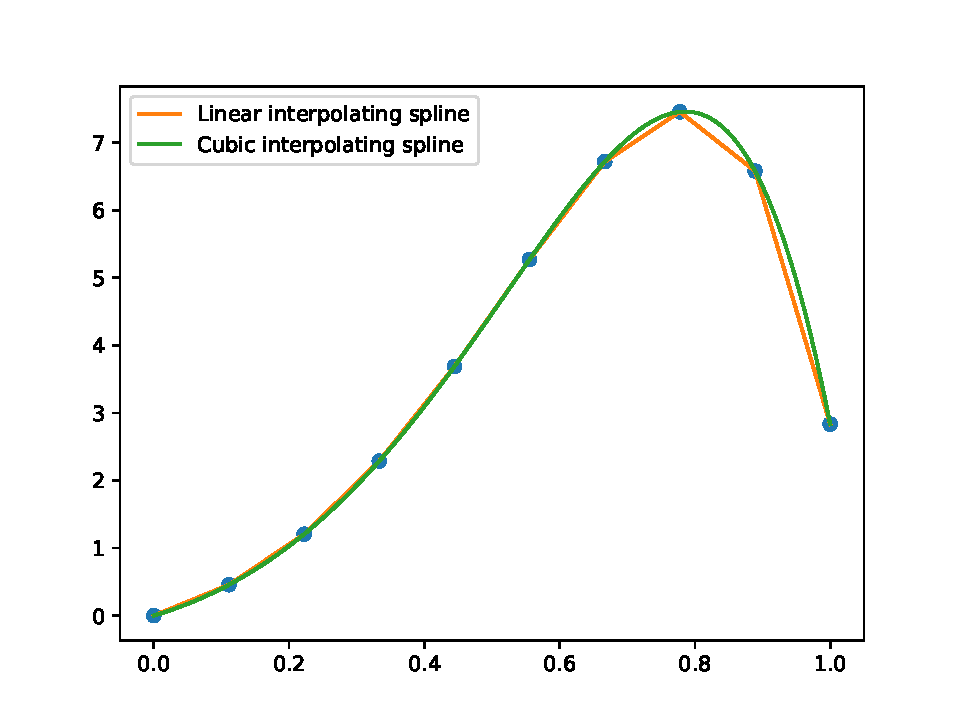
\includegraphics[width=0.7\textwidth]{lez6/spline.pdf}
\end{center}  
  
  \begin{itemize}
  \item Defined piecewsise by polinomials of degree k ($k = 3$ fairly popular)
    \begin{itemize}
    \item Interpolating: passing through a set of pre-defined points
    \item First $k-1$ derivatives continuos at the control points
    \end{itemize}
  \item Superior to polynomial interpolation or curve fitting in many cases
  \end{itemize}

\subsection{Splines: construction and properties}

\inputminted{python}{snippets/spline.py}
\begin{minted}{bash}
[Output]
1.3192110648078448
2.6659857771053925
\end{minted}

  \begin{itemize}
  \item Evaluation is fairly inexpensive
    \begin{itemize}
    \item If the input $x$-array is sorted can do a binary search in
      \alert{O(log(N)) complexity}
    \end{itemize}
  \item Derivatives and integrals are easy
    \begin{itemize}
    \item Can be calculated \emph{exactly} by means of elementary
      arithmetic operations
    \end{itemize}
  \end{itemize}
  
\vfill

\begin{tcolorbox}[width=\textwidth,colback={white},title={References },colbacktitle=gray,coltitle=black]
  \begin{itemize}
  \item \url{https://numpy.org/}
  \item \url{https://www.scipy.org/}
  \item \url{https://docs.scipy.org/doc/numpy/reference/arrays.indexing.html}
  \item \url{https://docs.scipy.org/doc/numpy/user/basics.broadcasting.html}
  \item \url{https://docs.scipy.org/doc/scipy/reference/interpolate.html}
  \end{itemize}
\end{tcolorbox}

\newpage


\section{\textit{Gio 13 ott - Lezione 7}}

\section{Advanced Python Features}

\subsection{Errors and Exceptions}
  \begin{itemize}
    \item \alert{Error handling} is one of the most important problem to solve when designing a program
    \item What should I do when I piece of code fails?
    \item What does fail mean?
    \begin {itemize}
      \item Invalid input e.g. passing a path to a non existent file, or passing a string to a function for dividing numbers
      \item Valid output not found, e.g searching the position of the letter 'd' in the string 'elephant'
      \item Output cannot be find in a reasonable amount of time
      \item Runtime resource failures: network connection down, disk space ended\dots
    \end{itemize}
    \item Two phylosophies (historically):
    \begin{itemize}
      \item Return some \alert{error flag} (in different ways) to tell the user that something went wrong
      \item \alert{Exceptions}
    \end{itemize}
    \item Example: a typical convention for programs is to return 0 from the main if the execution was successful and an
          error code (integer number) otherwise
  \end{itemize}
  


\subsection{Error flags (no)}

\inputminted{python}{snippets/error_flags.py}
\begin{minted}{bash}
[Output]
3
-1
We all live in a
We all live in a Yellow Submarin
\end{minted}

\subsection{Problems of error flags}

    Error codes have their use (and are fine in some cases) but they suffer from a few issues:
    \begin{itemize}
      \item Choosing them is often arbitrary (and sometimes is difficult to make a sensible choice)
      \begin{itemize}
        \item What if all the numbers can represent meaningful output of the function?
      \end{itemize}
      \item Are cumbersome to use
      \begin{itemize}
        \item Which error flag is used by a function? 0? -1? 99999999? $\rightarrow$ you have to go through the documentation for each!
        \item If you have a deep hierarchy of functions you have to perform checks and pass the error up at every level!
      \end{itemize}
      \item What if the caller of a function does not check the error flag?
      \begin{itemize}
        \item The bug can propagate \alert{silently} through its code!
      \end{itemize}
    \end{itemize}
    \medskip
    We want something that:
    \begin{itemize}
      \item Is clearly separated from the returned output
      \item Cannot be silently ignored by the user
      \item Is easy to report to upper level without lots of lines of code
    \end{itemize}  

\subsection{A different way}

\inputminted{python}{snippets/exceptions_vs_err_flags.py}
\begin{minted}{bash}
[Output]
We all live in a
Traceback (most recent call last):
    File "snippets/exceptions_vs_err_flags.py", line 11, in <module>
        print(cut_before(’We all live in a Yellow Submarine’, ’Red’))
    File "snippets/exceptions_vs_err_flags.py", line 5, in cut_before
    pos = input_string.index(substring)
ValueError: substring not found
\end{minted}

La filosofia base di Python è evitare di inventare delle cose.\\
Come faccio ad intercettare questo value error e in quel caso a fargli fare qualcosa di specifico?\\

\subsection{Eccezioni}

  \begin{itemize}
    \item An exception is an object that can be \alert{raised} (in other languages also \textit{thrown}) by
          a piece of code to signal that something went wrong
    \item When an exception is raised the normal flow of the code is interrupted
    \item The program automatically propagate the exception back in the function hierarchy
          until it found a place where the exception is  \alert{catched} and handled
    \item If the exception is never catched, not even in the main, the program crash \alert{with a specific error message}
    \item Cathcing the exception is done with a \emph{try - except} block
  \end{itemize}
  
Se non intercettiamo l'eccezione, il flusso del codice viene interrotto.
Possiamo dire "se ho questa eccezione allora faccio questo...".

\subsection{Try block}


\inputminted{python}{snippets/exceptions_brief.py}
\begin{minted}{bash}
[Output]
This line is not executed if an exception is raised in the try block
This line is executed only if a ValueError is raised in the try block
\end{minted}

Per ogni try possiamo anche mettere più di un except.\\
Dobbiamo cercare di intercettare le eccezioni nel modo più specifico possibile!

\subsection{\texttt{else}, \texttt{finally}}

  \begin{itemize}
    \item There are two more optional statements in a try-block:
    \medskip
    \begin{itemize}
      \item \emph{else}: executed only if no exception is raised in the try block
      \medskip
      \item \emph{finally}: executed no matter what
      \medskip
    \end{itemize}
    \item \emph{finally} is executed even if there is a return statement in the try
          block
    \item can be used to release important resources (e.g. closing a
          file, or a connection)
  \end{itemize}

\subsection{Using \texttt{else} and \texttt{finally}}

\inputminted{python}{snippets/exceptions.py}
\begin{minted}{bash}
[Output]
This line
This line
This line
This line
This line
A. Manfreda (INFN)
is
is
is
is
is
not executed if an exception is raised in the try block
executed only if no exception is raised in the try block
always executed
executed only if a ValueError is raised in the try block
always executed
\end{minted}


L'eccezione è un oggetto. E dentro di essa possiamo encapsulare tutte le informazioni necessarie per capire cosa è andato storto!



\subsection{The beauty of exceptions}
  \begin{itemize}
    \item If that was all, exceptions would only be moderately useful
    \item The real bargain is that you can send back information together with the exception
    \item In fact you \textit{are sending a full object}: the excetpion iteslf. Surprised?
    \item Inside the exception you can report all kind of data useful to reconstruct the exact error,
          which can be used by the caller for debug or to produce meaningful error messages
    \item You can also select which exceptions you catch, leaving the others propagate up
    \item Python provides a rich hierarchy of exception classes, which you can further customize
          (if you want) by deriving your own subclasses
  \end{itemize}

\subsection{The family tree of Python exceptions}

\begin{figure}[ht]
    \centering
    
\includegraphics[width=1\textwidth]{lez7/error_tree.png}
    \caption{family tree}
    \label{error_tree}
\end{figure}
\FloatBarrier


\subsection{Catching specific exceptions}

\inputminted{python}{snippets/try_block.py}
\begin{minted}{bash}
[Output]
[Errno 2] No such file or directory: ’i_do_not_exist.txt’
\end{minted}

\texttt{Exception} sta per qualsiasi altro tipo di errore.


\subsection{Exception caveats}
  \begin{itemize}
    \item Warning: catching \emph{Exception}, will also catch \emph{SyntaxError}
          and \emph{NameError}
    \medskip
    \item This mean that the code will 'run' even if there is a typo in it!
    \medskip
    \item Bottom line: \alert{you should never catch generically for \emph{Exception}},
          always be more specific
    \medskip
    \item Even worse, you should never catch for \emph{BaseException} as
          that would even prevent the user for from aborting the execution with a
          \emph{KeyboardInterrupt} (e.g. Ctrl-C)
    \medskip
    \item Unless that is what you need, of course
  \end{itemize}
  
  
  \subsection{There is no check - only try}
  \begin{itemize}
    \item In Python exceptions are the default methods for handling failures
    \smallskip
    \item Many functions raise an exception when something goes wrong
    \smallskip
    \item The common approach is: do not chech the input beforehand. Use it and
          be ready to catch exceptions if any.
    \smallskip
    \item \textit{Easier to ask for forgiveness than permission.} 
  \end{itemize}
  
  
\subsection{Catching specific exceptions}

\inputminted{python}{snippets/dont_ask_permission.py}
\begin{minted}{bash}
[Output]
Oops - file ’i_do_not_exists.txt’ does not exist
Oops - cannot read the file!
[Errno 2] No such file or directory: ’i_do_not_exists.txt’
\end{minted}


%%%%% slide saltate


\subsection{Raising exceptions}
  \begin{itemize}
    \item Up to now we have been dealing with exceptions generated by Python
          functions
    \medskip
    \item What about raising exceptions ourselves?
  \end{itemize}
  
\inputminted{python}{snippets/raising.py}
\begin{minted}{bash}
[Output]
this is a useful debug message
\end{minted}

Valutare bene prima di mettere \texttt{sys.exit('guarda che ho bisogno di quel file')}. Se invece sollevo un'eccezione, offro la scelta a chi esegue il codice.\\

\subsection{Custom exceptions}
  \begin{itemize}
    \item Beside the built-in exceptions provided by Python, you can add your
          own custom exceptions by inheriting from the \emph{Exception} class
    \medskip
    \item This serves two purposes:
    \begin{itemize}
      \item Make the exception handling code more specific, and hence more
            readible
      \item Allows you to pass additional data with your exception - in the
            form of attributes of the class - which can be used for debug
            or any other purpose
    \end{itemize}
  \end{itemize}

\inputminted{python}{snippets/custom_exceptions.py}
\begin{minted}{bash}
[Output]
Traceback (most recent call last):
File "snippets/custom_exceptions.py", line 4, in <module>
raise SimpleCustomError(’simple error’)
__main__.SimpleCustomError: simple error
\end{minted}

\textbf{altro esempio:}

\inputminted{python}{snippets/custom_exceptions_2.py}
\begin{minted}{bash}
[Output]
ValueTooLargeError: 100 is too large
\end{minted}


\subsection{Where to catch exceptions?}
  \begin{itemize}
    \item Differently from error flags, which need to be checked as early as
          possible, you are not in a rush with exceptions
    \item Remeber: your goal is to provide the user a meaningful error message and
          useful debug information.
    \item You should catch an exception only when you have enough context to
          do that - which sometimes means waiting a few levels in the hierarchy!
  \end{itemize}

I blocchi try-except devono essere il più piccolo possibile, e il più specifico possibile!

%%%%%%

\subsection{When to catch}

\inputminted{python}{snippets/when_to_catch.py}
\begin{minted}{bash}
[Output]
0.1 15.2
0.2 12.4
Traceback (most recent call last):
File "snippets/when_to_catch.py", line 12, in <module>
time, tension = parse_line(line)
File "snippets/when_to_catch.py", line 6, in parse_line
tension = float(values[1])
ValueError: could not convert string to float: ’pippo’
\end{minted}

\subsection{Catch too early}

\inputminted{python}{snippets/when_to_catch_1.py}
\begin{minted}{bash}
[Output]
0.1 15.2
0.2 12.4
could not convert string to float: ’pippo’
Traceback (most recent call last):
File "snippets/when_to_catch_1.py", line 15, in <module>
time, tension = parse_line(line)
TypeError: ’NoneType’ object is not iterable
\end{minted}

\subsection{Catch when needed}

\inputminted{python}{snippets/when_to_catch_2.py}
\begin{minted}{bash}
[Output]
0.1 15.2
0.2 12.4
Line 3 error: could not convert string to float: ’pippo’
0.4 13.2
\end{minted}

\newpage
\section{\textit{Lun 17 ott - Lezione 8}}

\section{Iterators}

Quando una classe implementa il metodo \texttt{\_\_iter\_\_} allora diventa \textit{iterabile}.

  \subsection{Iterators and iterables}
Un iteratore è un oggetto definito dal fatto di sapere qual è il prossimo elemento, grazie al metodo magico \texttt{\_\_next\_\_}.  

  \begin{itemize}
    \item An \emph{iterable} in Python is something that has a \emph{\_\_iter\_\_}
          method, which returns an \alert{iterator}
    \item An \emph{iterator} is an object that implement a \emph{\_\_next\_\_} method
          which is used to retrieve elements one at the time
    \item When there are no more elements to return, the iterator signals that with a specific
          exception: \emph{StopIteration()}
    \item An iterator also implement an \emph{\_\_iter\_\_} method that return\dots itself.
          So an iterator is also technically an iterable%
          \footnote{Only 'technically' because an iterator has no data of its
          own, so you always need a 'real' iterable to actually iterate}%
          ! (But the opposite is not true)
  \end{itemize}

Perché passare dall'iteratore? Perché non implementare il metodo \texttt{\_\_next\_\_} direttamente sul nostro oggetto? Il fatto è che posso avere più iteratori attivi su uno stesso contenitore dati. Per questo non posso implementare il metodo \texttt{\_\_next\_\_} direttamente nella classe di dati, ma devo passare per l'iteratore.

\subsection{A 'for' loop unpacked}

\inputminted{python}{snippets/show_iterator.py}
Salvo il mio iteratore in una variabile e inizio un ciclo (potenzialmente infinito). Quando l'iterazione solleva l'eccezione \texttt{StopIteration} interrompo il ciclo.
\begin{minted}{bash}
[Output]
1.0
2.0
3.0
1.0
2.0
3.0
\end{minted}

\subsection{A simple iterator}


\inputminted{python}{snippets/simple_iterator.py}
Nel costruttore gli passo il contenitore di dati su cui voglio iterate. Mi salvo una referenza a questo contenitore dati. E faccio partire l'indice da zero.
Nota: questo funziona per le liste, tuple e array, ma non per i dizionari, che non restituiscono \texttt{indexError}, ma \texttt{KeyError}!


\inputminted{python}{snippets/test_simple_iterator.py}

\begin{minted}{bash}
[Output]
1.0
2.0
3.0
stella
\end{minted}

\subsection{A crazy iterator}
\inputminted{python}{snippets/crazy_iterator.py}

\inputminted{python}{snippets/test_crazy_iterator.py}

\begin{minted}{bash}
[Output]
B
E
A
C
A
D
D
D
\end{minted}

\subsection{Python tools for iterables}

  \begin{itemize}
    \item Python provides a number of functions that consume an iterable and return a single value:
    \begin{itemize}
      \item \texttt{sum}: Sum all the elements
      \item \texttt{all}: Return true if a given condition is true for all the elements
      \item \texttt{any}: Return true if a given condition is true for at lest one element
      \item \texttt{max}: Return the max
      \item \texttt{min}: Return the minimum
      \item \texttt{functools.reduce}: Apply a function recursively to pairs of elements
    \end{itemize}
  \end{itemize}

\section{Generatori}

Gli iteratori operano su dati \textbf{esistenti}. Tuttavia, a volte vorremmo iterare su qualcosa che non esiste già da prima. Ad esempio, se vogliamo generare in maniera iterativa tutti i numeri della serie di Fibonacci; ad ogni iterazione vogliamo generare il prossimo.\\
Questa cosa non si può fare con gli iteratori, ma si fa con i \textbf{generatori}:\\\

  \begin{itemize}
    \item We have seen that iterators are useful to iterate over container
    \item However that assumes a containers exists $\rightarrow$ memory usage
    \item \alert{Generators} allow you to loop over sequences of items even when
          they don't exist before - the items are just created \alert{lazily} the
          moment they are required (\textbf{lazy:} una cosa che viene fatta all'ultimo momento possibile.)
    \item For example you can write a generator to loops over the Fibonacci
          succession. You can't create the sequence earlier, since it is not
          finite!
    \item Generators are created through either \alert{generator expressions} or
          \alert{generator functions}
    \item In real life most of the time you will simply use pre-made functions
          that return a generator, like \emph{range()} (in Python 3)
    \item Generator can be used to iterate in for loops, just like iterators
  \end{itemize}


\subsection{Generators first look}

Sui generatori possiamo iterare esattamente come sugli iteratori: la sintassi è la stessa.\\

\inputminted{python}{snippets/generators.py}

\begin{minted}{bash}
[Output]
0
1
2
3
144
1
25
\end{minted}


\subsection{Generator functions}

  \begin{itemize}
    \item A \alert{generator function} is a function that contains the keyword \alert{yield} at
          least once in his body
    \item When you call a generator function the code is not executed - instead
          a generator object is created and returned (even if you don't have a return statement)
    \item Each call to \emph{next()} on the returned generator will make the function code 
          run until it finds a \emph{yield} statement
    \item Then the execution is paused and the value of the expression on the right 
          of \emph{yield} is returned (yielded) to the caller
    \item A further call of next will resume the execution from where it was suspended
          until the next \emph{yield} and so on
    \item Eventually, when the function body ends, \emph{StopIteration} is raised
    \item Usually generators functions contain a loop - but it's not mandatory!
  \end{itemize}

Quando noi chiamiamo una funzione generatrice, non viene eseguito il corpo della funzione, bensì viene restituito un generatore.

\inputminted{python}{snippets/generator_functions.py}

\begin{minted}{bash}
[Output]
First call
1
Second call
2
I am about to rise a StopIteration exception...
Traceback (most recent call last):
    File "snippets/generator_functions.py", line 11, in <module>
        next(gen) # The third next() will throw StopIteration
StopIteration
\end{minted}


\subsection{Infinite sequence generators}

Tipicamente all'interno del generatore c'è un loop.

\inputminted{python}{snippets/fibonacci.py}

\begin{minted}{bash}
[Output]
[0, 1, 1, 2, 3, 5, 8]
[0, 1, 1, 2, 3, 5, 8]
\end{minted}

islice prende un certo numero di elementi da un iteratore.\\

Un generatore serve in tutti quei casi in cui voglio generare i vari elementi in maniera lazy.\\

  \subsection{Python generator functions}
  
  \begin{itemize}
    \item Python provides a number of built-in functions that return a generator from an iterable, such as:
    \begin{itemize}
      \item \texttt{enumerate}: Automatic counting of iterations
      \item \texttt{map}: Apply a function to the elements
      \item \texttt{filter}: Return only the elements passing a given condition
      \item \texttt{zip}: Return pairs of elements (requires two sequences)
      \item \texttt{reversed}: Loop in the reversed order
    \end{itemize}

    \item Countless others can be found in the \alert{\texttt{itertools}} library
    \begin{itemize}
      \item \texttt{islice}: Slice the loop with start, stop and step
      \item \texttt{takewhile}: Stop looping when a condition becomes false
      \item \texttt{accumulate}: Get the results of applying the function iteratively to pair of elements
      \item \texttt{chain}: Loop through many sequences one after another
      \item \texttt{cycle}: Loop over the sequence repeatedly, indefinitely
      \item \texttt{permutations}: Get all the permutations of a given length
      \item \texttt{product}: Compute the cartesian product of iterables
      \item \texttt{groupby}: Group by value of some key (function)     
      \item And so on\dots
    \end{itemize}
    
    \medskip
    
    \item Take a look at the documentation of each function to see how to 
          properly call it!
  \end{itemize}  

\subsection{Itertools showcase}

\inputminted{python}{snippets/itertools_showcase.py}

\begin{minted}{bash}
[Output]
[1, 3, 6, 10]
[1, 2, 6, 24]
[(1, 2, 3), (1, 2, 4), (1, 3, 4), (2, 3, 4)]
[(5, 6), (6, 5)]
[(1, 5), (1, 6), (2, 5), (2, 6), (3, 5), (3, 6), (4, 5), (4, 6)]
False [1, 3, 5]
True [2, 4, 6]
\end{minted}

\section{Lambda functions}

Sono un modo per creare una funzione anonima (senza un nome).

  \begin{itemize}
    \item \alert{Anonymous functions}, or \alert{lambda functions} are a construct typical of \alert{functional programming}
    \item \url{https://en.wikipedia.org/wiki/Lambda_calculus}
    \item \url{https://en.wikipedia.org/wiki/Functional_programming}
    \item In Python a lambda function is essentially a special sintax for creating a function
          on the fly, without giving it a name
    \item They are limited to \alert{a single expression}, which is returned to the user
    \item Many of the typical uses for lambdas are already covered in python by generator expressions and comprehension,
          so this is more like a niche feature of the language
  \end{itemize}
  

\inputminted{python}{snippets/lambda.py}
Il corpo di una funzione deve essere solo una riga.\\
\texttt{lambda argomenti: output}
\begin{minted}{bash}
[Output]
-5
[0, 1, 4, 9, 16, 25, 36, 49, 64, 81]
[0, 1, 4, 9, 16, 25, 36, 49, 64, 81]
\end{minted}

\subsection{Recap example: file iterator}

\inputminted{python}{snippets/file_iterator.py}

\begin{minted}{bash}
[Output]
0 0.1 15.2
1 0.2 12.4
Line 1 error: could not convert string to float: ’pippo’
\end{minted}

\subsection{File iterator redone}


\inputminted{python}{snippets/file_iterator_2.py}

\begin{minted}{bash}
[Output]
0.1 15.2
0.2 12.4
Line 3 error: could not convert string to float: ’pippo’
0.4 13.2
\end{minted}


\subsection{File iterator, final version}

\inputminted{python}{snippets/file_iterator_3.py}

\begin{minted}{bash}
[Output]
0.1 15.2
0.2 12.4
Line 3 error: could not convert string to float: ’pippo’
0.4 13.2
\end{minted}

\section{Decorators}
\textit{non ha avuto tempo di farli tutti, vediamo solo:}
  \subsection{The @classmethod decorator}
costruttore alternativo
  \begin{itemize}
    \item We have already seen a built-in Python decorator: \emph{@property}
    \item We used that to get proper encapsulation
    \item There is another built-in decorator one which is very useful for classes: \alert{\emph{@classmethod}}
    \item A classmethod is like a class attribute: you don't need an instance to
          use it
    \item A class method can access class attributes but not instance attributes
    \item The main use for class methods is to provide \alert{alternate constructors}
  \end{itemize}


\inputminted{python}{snippets/classmethod.py}

\begin{minted}{bash}
[Output]
<class ’__main__.LabData’>
[15.2 12.4 11.7 13.2]
\end{minted}



\chapter{Parallel Computing}
%\vspace{10.5cm}


\section{\textit{Gio 20 ott - Lezione 9}}
\section{Computer architecture from a
performance point of view: from
serial to parallel}
\sectionmark{from
serial to parallel}

\subsection{Architettura di Von Neumann}
L'architettura di Von Neumann è una tipologia di architettura hardware per computer digitali programmabili a programma memorizzato la quale condivide i dati del programma e le istruzioni del programma nello stesso spazio di memoria, contrapponendosi all'architettura Harvard nella quale invece i dati del programma e le istruzioni del programma sono memorizzati in spazi di memoria distinti. 
Introdotta nel 1945 da John Von
Neumann, consiste di 5 elementi:
\begin{enumerate}
    \item Processing unit (arithmetic logic
unit)
    \item Control unit (instruction pool)
    \item Memory
    \item Bus
    \item I/O
\end{enumerate}

\begin{figure}[ht]
    \centering
    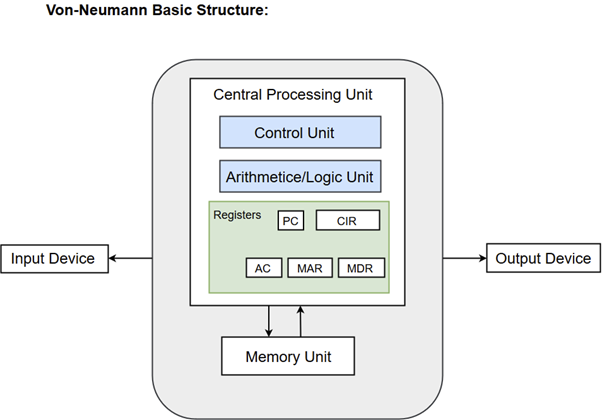
\includegraphics[width=0.6\textwidth]{figure_parallel/VN_arch.png}
\end{figure}
\FloatBarrier


Da una parte abbiamo i dati, dall'altra abbiamo i programmi. La parte di controllo copia i dati dalla memoria in una memoria temporanea e vi esegue i comandi contenuti nei programmi.\\

\subsection{Von Neumann Bottleneck}
L'architettura di Von Neumann presenta delle limitazioni legate al fatto che viene condiviso lo stesso bus per dati e istruzioni, creando il cosiddetto \textit{Von Neumann Bottleneck}.\\



\begin{figure}[ht]
    \centering
    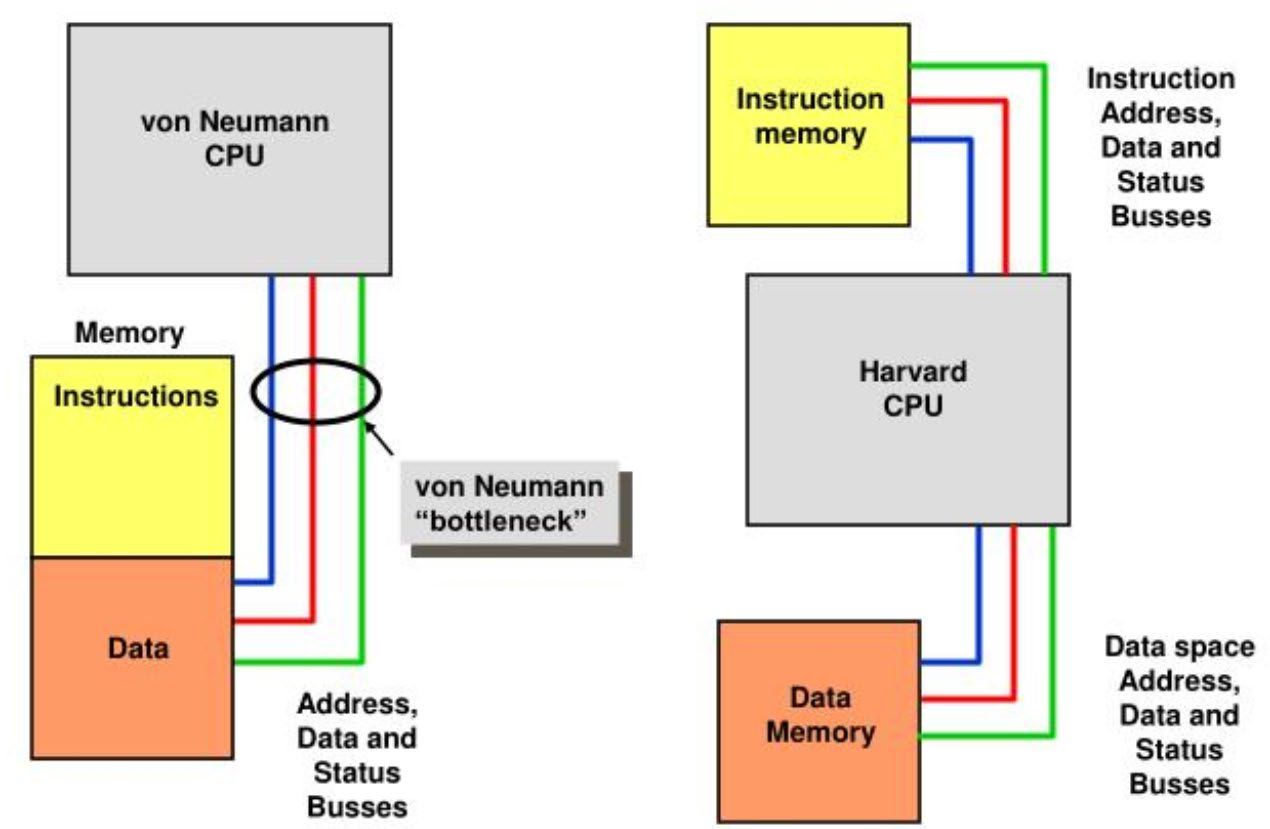
\includegraphics[width=0.6\textwidth]{figure_parallel/bottleneck.png}
\end{figure}
\FloatBarrier


Esistono varie strategie per mitigare questo fenomeno:
\begin{enumerate}
    \item Caching and memory gerarchy on chip
    \item Separate access to data and instructions (Harvard Architecture)
    \item Branch prediction
\end{enumerate}

\subsection{Simple Server architecture}
In a server multiple components interacts during the program execution.
\begin{itemize}
    \item Processors/cores
    \begin{itemize}
        \item I-cache, D-cache
    \end{itemize}
    \item Shared Caches
    \begin{itemize}
        \item For instruction and data
    \end{itemize}
    \item Memory controllers
    \item I/O subsystems
        \begin{itemize}
        \item Storage, network, peripherals
    \end{itemize}
\end{itemize}

\begin{figure}[ht]
    \centering
    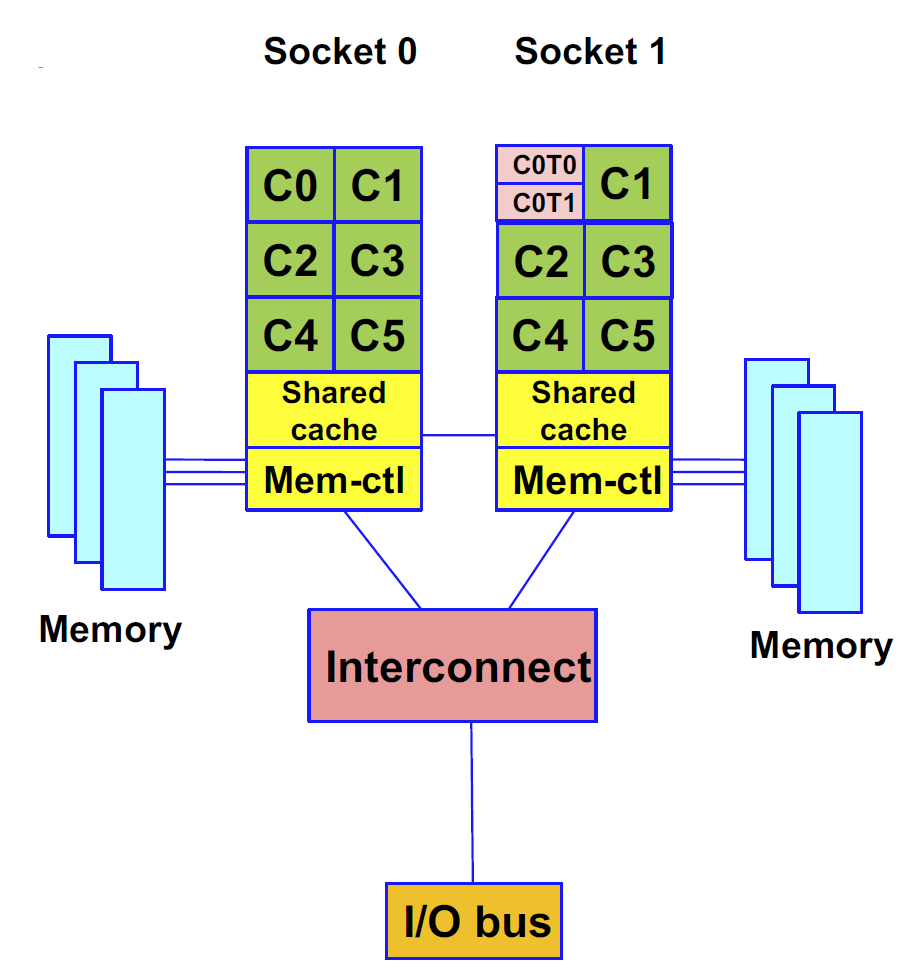
\includegraphics[width=0.5\textwidth]{figure_parallel/server.png}
\end{figure}
\FloatBarrier

An example: NUMA architecture (non-
uniform memory access).

\subsection{Memoria}
Ci sono 2 parametri che caratterizzano le memorie:\\ 
\textbf{Banda:} numero di byte che posso estrarre dalla memoria ad ogni colpo di clock.\\
\textbf{Latenza:} quanto tempo ci vuole dopo che abbiamo richiesto i dati ad ottenerli effettivamente.\\

Se ho un'operazione che eseguo molto spesso, non conviene ogni volta accedere a questa operazione.
Analogamente, se abbiamo gli stessi dati su cui fare delle operazioni, li carichiamo nella cache una volta sola e poi facciamo le operazioni.\\

In particolare, la cache è strutturata su più livelli, ognuno dei quali ha performance diverse in termini di Banda e Latenza.\\
La gerarchia di "data access" e "instruction fetching" è fondamentale nell'architettura dei computer.\\

\begin{figure}[ht]
    \centering
    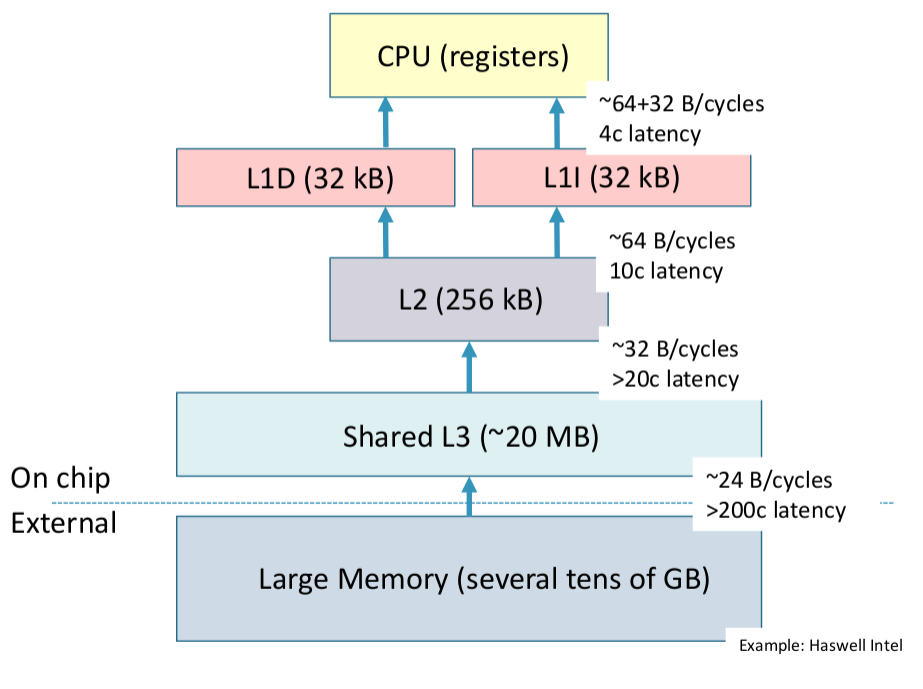
\includegraphics[width=0.6\textwidth]{figure_parallel/cache.png}
\end{figure}
\FloatBarrier

Più il clock va veloce e più il processore è veloce. Tuttavia la velocità del clock non può aumentare all'infinito. Si cercano metodi per andare più veloci del tempo scandito dal clock.\\

\subsection{Seven dimensions of performance}
The «modern» PC performance depends on (at least) seven characteristics:

\begin{figure}[ht]
    \centering
    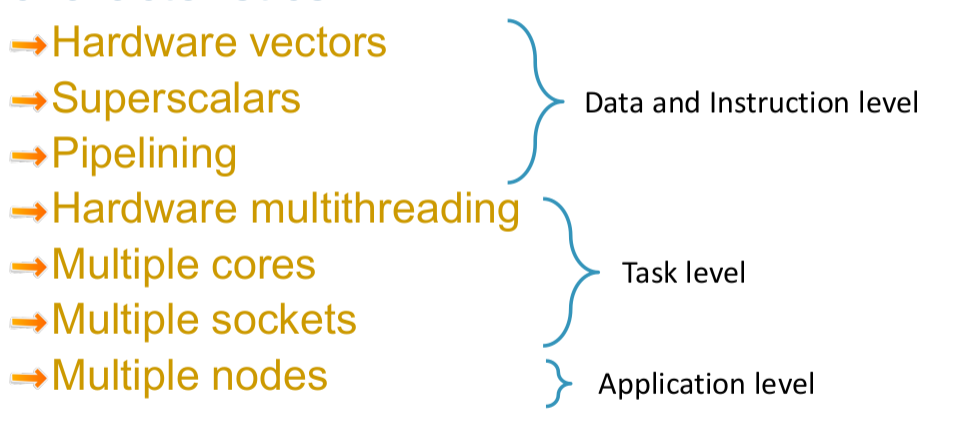
\includegraphics[width=0.6\textwidth]{figure_parallel/7perf.png}
\end{figure}
\FloatBarrier

\subsection{Processori Vettoriali}
Finora abbiamo visto processori "scalari".\\
Modern processors implement registers for vectorialization (SSE/SSE2 and
AVX)

\begin{itemize}
    \item Scalar mode:
    \begin{itemize}
        \item One operation produces one result
    \end{itemize}
    \item SIMD (Single Instruction Multiple Data) is a simple way to parallelize
    \begin{itemize}
        \item One operation produces multiple results
    \end{itemize}
\end{itemize}

\begin{figure}[ht]
    \centering
    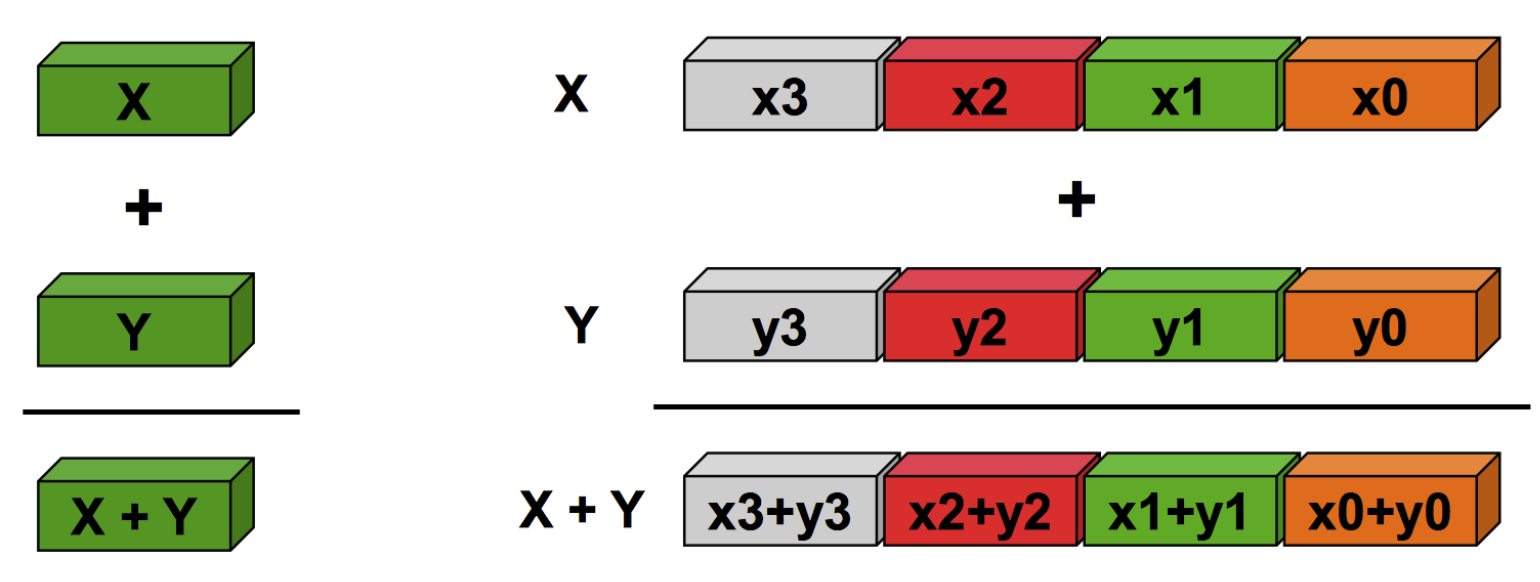
\includegraphics[width=0.7\textwidth]{figure_parallel/vector_sum.png}
\end{figure}
\FloatBarrier

\subsection{Superscalari}
Abbiamo tanti processori scalari, ognuno dei quali fa singole operazioni su singoli elementi di memoria. \\

\begin{figure}[ht]
    \centering
    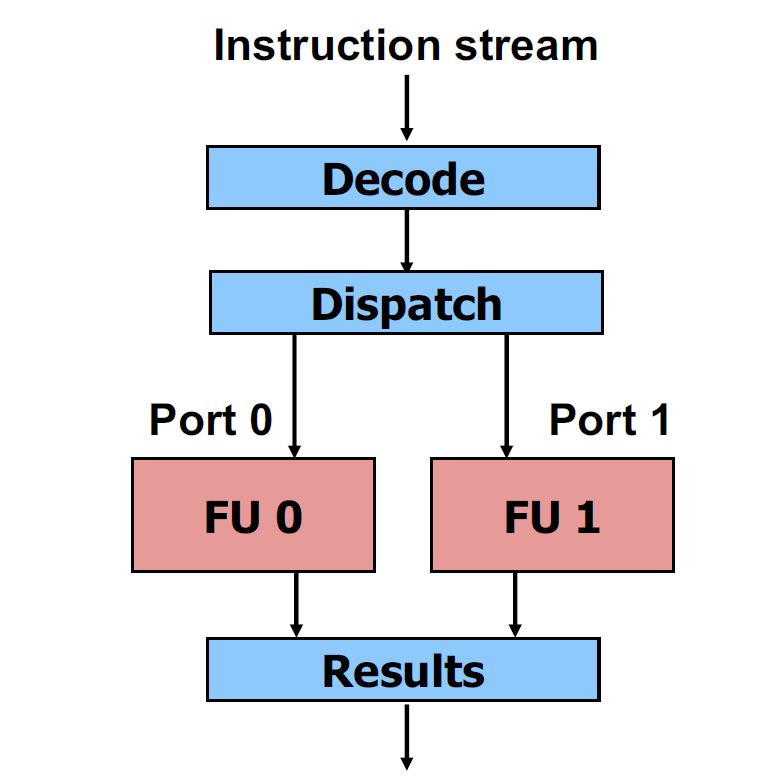
\includegraphics[width=0.4\textwidth]{figure_parallel/superscalar.png}
\end{figure}
\FloatBarrier

\begin{itemize}
    \item Architecture between pure «scalar» and pure «vector»
    \begin{itemize}
        \item Several hardware units can execute different operation on different data at the same time
    \end{itemize}
\end{itemize}




\begin{itemize}
    \item Functional Units (FU) can have identical or different computing capabilities
    \begin{itemize}
        \item Decoder and Dispatcher must have the capability to manage two instruction in one clock cicle
    \end{itemize}
\end{itemize}

\begin{itemize}
    \item Usefull for Branch Prediction
    \begin{itemize}
        \item Execute at the same time different branches in an algorithm then choose the correct one
    \end{itemize}
\end{itemize}



\textbf{Branch prediction}:
Ho sufficienti risorse per eseguire contemporaneamente varie branch di un programma.

\subsection{Pipelining}


Pipelining consists in the capability to execute different stage of consecutive instructions at the same time.

\begin{figure}[ht]
    \centering
    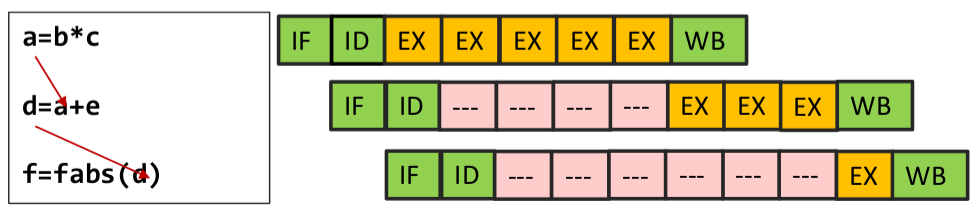
\includegraphics[width=0.7\textwidth]{figure_parallel/pipeline.png}
\end{figure}
\FloatBarrier

The pipeline is an important ingredient in
modern processors. However, it isn’t always possible to fully exploit the pipeline.

\begin{figure}[ht]
    \centering
    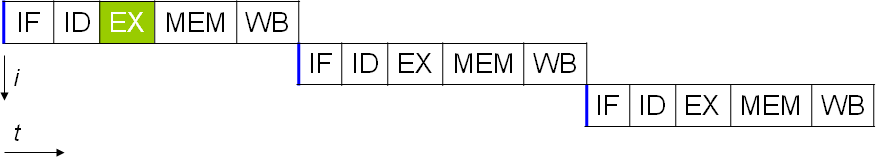
\includegraphics[width=0.5\textwidth]{figure_parallel/pipeline1.png}
    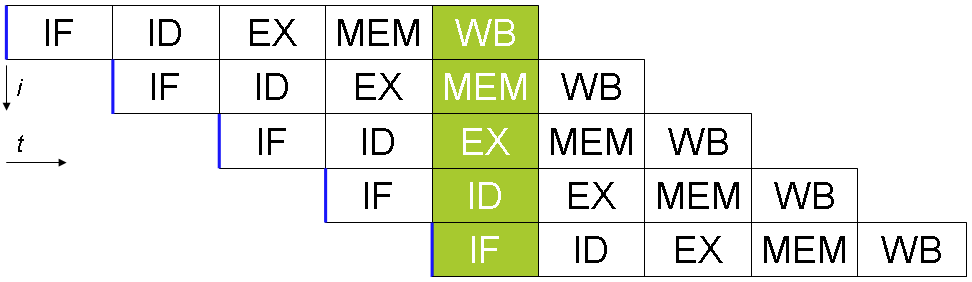
\includegraphics[width=0.5\textwidth]{figure_parallel/pipeline2.png}\end{figure}
\FloatBarrier


\begin{tcolorbox}[width=\textwidth,colback={white},title={Summary: },colbacktitle=cyan,coltitle=black]
  \begin{itemize}
    \item Superscalars, Pipelining and Vectorialization are methods to exploit some «parallelism» at the instruction and data level: ILP
    \begin{itemize}
        \item Probably OOO (Out-of-order) execution should be included in this category
    \end{itemize}
    \item The possible improvement thanks to ILP depends on problem and data structures
    \begin{itemize}
        \item 1x-10x for Superscalars and Pipeline
        \item 2x,4x,8x,16x for the vectorialization
    \end{itemize}
    \item These methods show «saturation» because they are limited by the CPU resources available
        \begin{itemize}
        \item Pentium 4: 30 pipeline stages (nowadays 10-15 maximum)
        \item ARM A57 (Apple A7/A8): 9 ports/6 instructions superscalar
        \item Intel Tiger Lake: vector of 512 bits for a subset of AVX512 instructions
    \end{itemize}
   \end{itemize}  
   … the point is: can CPU resources grow indefinitely?
\end{tcolorbox}


\subsection{Dennard Scaling}

\begin{wrapfigure}{r}{0.4\textwidth}
  \begin{center}
    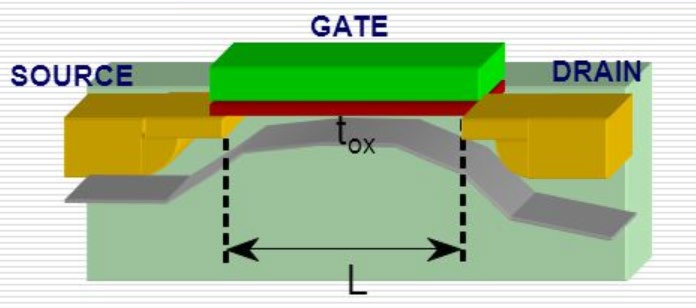
\includegraphics[width=0.35\textwidth]{figure_parallel/fet.png}
  \end{center}
\end{wrapfigure}

Aka MOSFET scaling (Dennard scaling after an article from Dennard et al. in 1974 in IEEE Journal of Solid State Circuits)\\
\textbf{-In each generation of CMOS based IC the power
consumption remains the same}\\
Breakdown of Dennard scaling around 2006: With very small integration it is not true anymore that the power consumption is the same, due to increasing in current leakage. The increasing of the speed of the transistors switching (frequency) is not anymore linear with the performance of the CPU\\

Energy consumption has become more important to users (For mobile, IoT, and for large clouds).\\
Processors have reached their power limit: Thermal dissipation is maxed out (chips turn off to avoid
overheating!). Even with better packaging: heat and battery are limits.

\begin{figure}[ht]
    \centering
    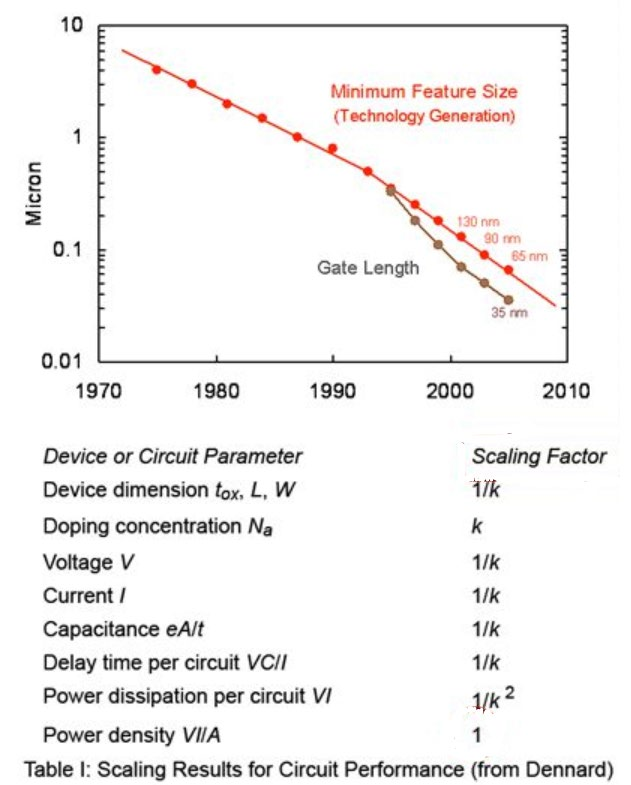
\includegraphics[width=0.4\textwidth]{figure_parallel/dennard.png}\end{figure}
\FloatBarrier

\subsection{Moore scaling}


Moore’s «law» is the empirical
observation that the number of
transistors doubles about each two
years (the performance of CPU doubles each 18 months).\\
Moore’s prediction was verified for
decades, however, around 2005 is starts to show saturation!\\
Moore's law is closely related to Dennard scaling.


\begin{figure}[ht]
\centering
\begin{subfigure}{.5\textwidth}
  \centering
  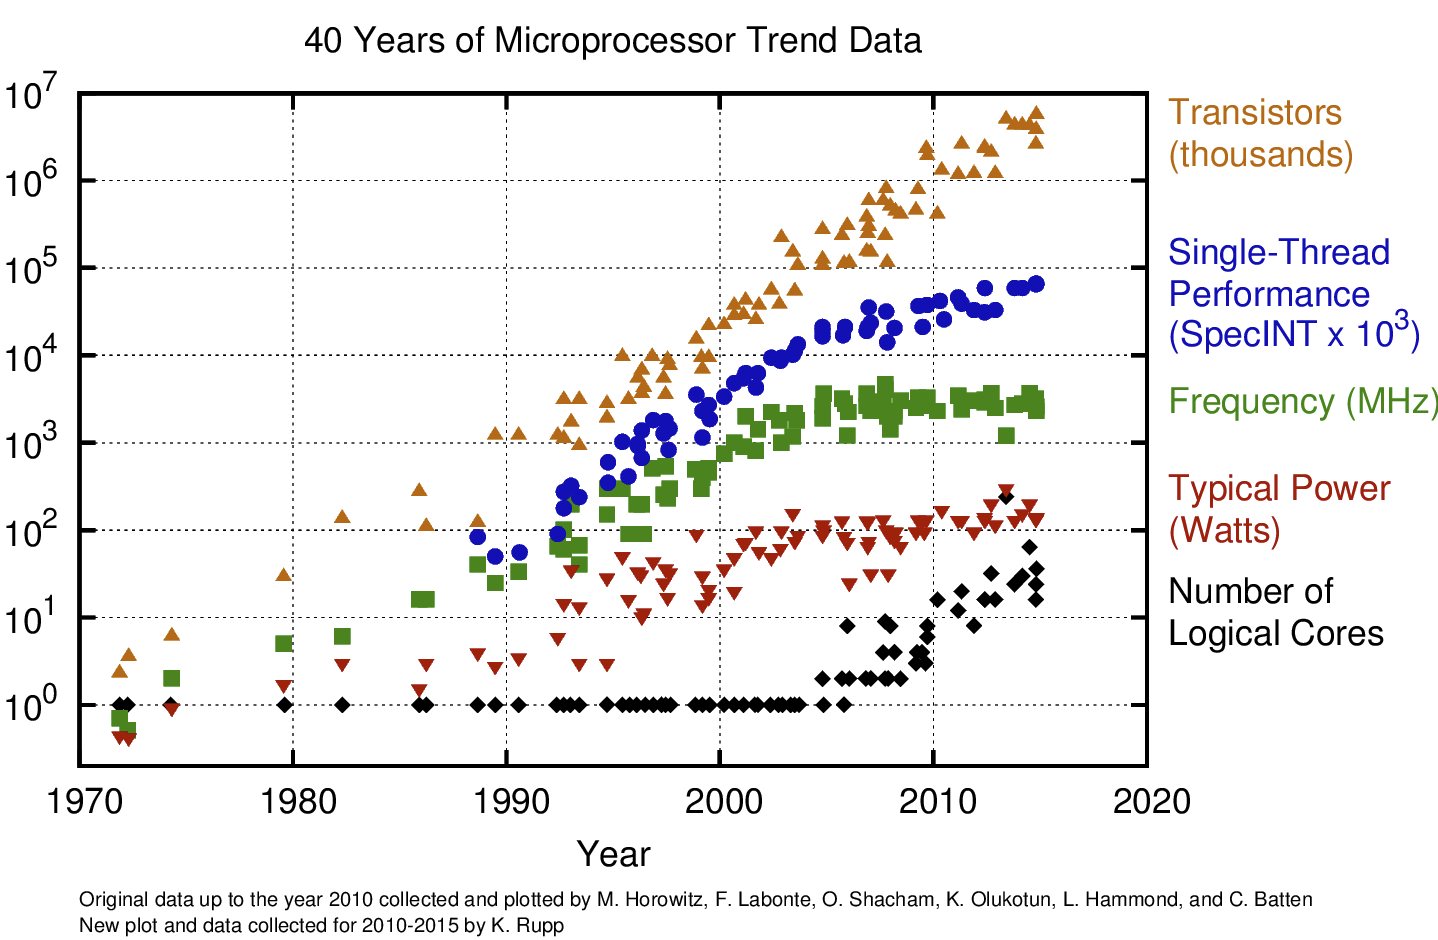
\includegraphics[width=.9\textwidth]{figure_parallel/moore.png}
\end{subfigure}%
\begin{subfigure}{.5\textwidth}
  \centering
  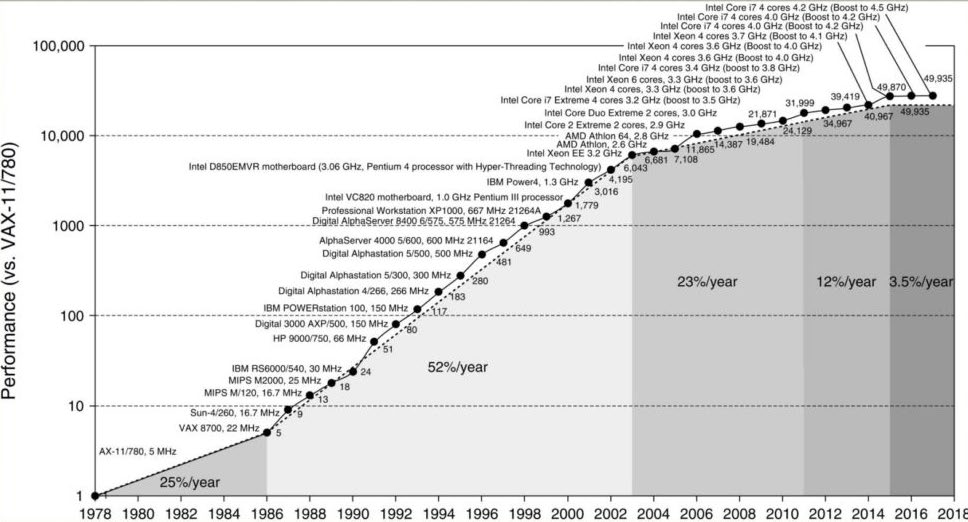
\includegraphics[width=.9\textwidth]{figure_parallel/moore2.png}
\end{subfigure}
\end{figure}

\subsection{Hardware parallelism}

How to avoid saturation?\\
Instruction level parallelism achieved significant performance advantages.But the performance are related to clock speed. Increasing in ILP is still possibile but the complexity of CPU is more than linear, diminishing return in efficiency.\\
\textbf{We need a next level in parallelism!}

\subsection{Flynn’s taxonomy}
Classification of computers architectures based on the number of data streams and instructions streams.
\begin{itemize}
    \item Single Instruction Single Data (SISD): Traditional sequential computing
    \item Singe Instruction Multiple Data (SIMD)
    \item Multiple Instructions Single Data (MISD)
    \item Multiple Instructions Multiple Data (MIMD)
\end{itemize}

\subsection{SISD: Single Instruction Single Data}
Only one instruction operates for
each time slot on one data (sequential processing).


\begin{figure}[ht]
\centering
\begin{subfigure}{.7\textwidth}
  \centering
  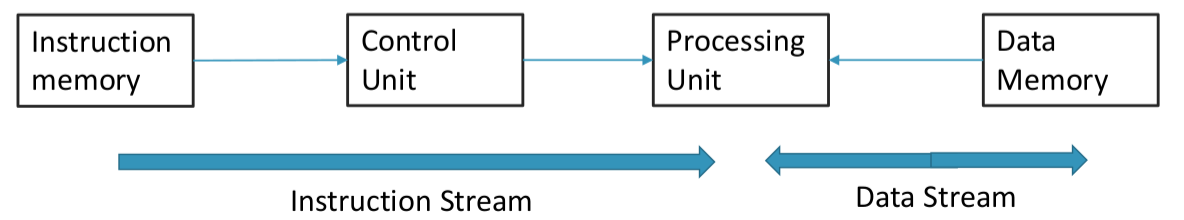
\includegraphics[width=.9\textwidth]{figure_parallel/sisd2.png}
\end{subfigure}%
\begin{subfigure}{.3\textwidth}
  \centering
  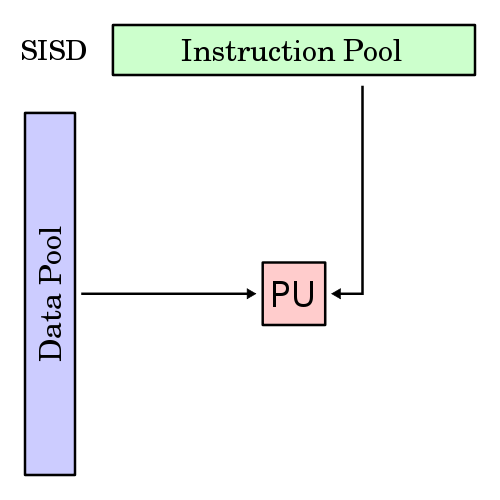
\includegraphics[width=.9\textwidth]{figure_parallel/SISD.png}
\end{subfigure}
\end{figure}

\subsection{SIMD: Single Instruction Multiple Data}

At one time one instruction operates on multiple data.

\begin{itemize}
    \item Very similar to vector processors (although in the vector architecture the parallelism is obtained with a pipeline, while in SIMD the operations are really parallel on vector’s element.)
    \item Array processors
    \item Most modern processors contain one or more SIMD sections
\end{itemize}

\begin{figure}[ht]
\centering
\begin{subfigure}{.7\textwidth}
  \centering
  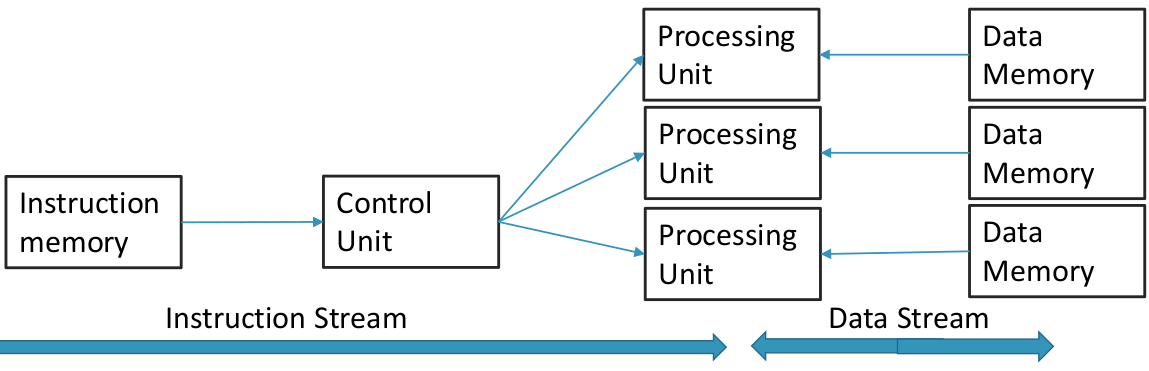
\includegraphics[width=.9\textwidth]{figure_parallel/simd.png}
\end{subfigure}%
\begin{subfigure}{.3\textwidth}
  \centering
  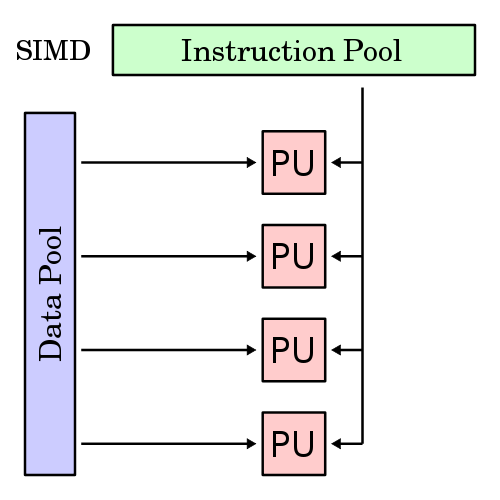
\includegraphics[width=.9\textwidth]{figure_parallel/simd2.png}
\end{subfigure}
\end{figure}

\subsection{MIMD: Multiple Instruction Multiple Data}

Multiple instructions streams operate on multiple data stream.
\begin{itemize}
    \item Most of supercomputers are organized as MIMD architecture
    \item Multi-core superscalar, multi-processors and distributed systems
\end{itemize}

\begin{figure}[ht]
\centering
\begin{subfigure}{.7\textwidth}
  \centering
  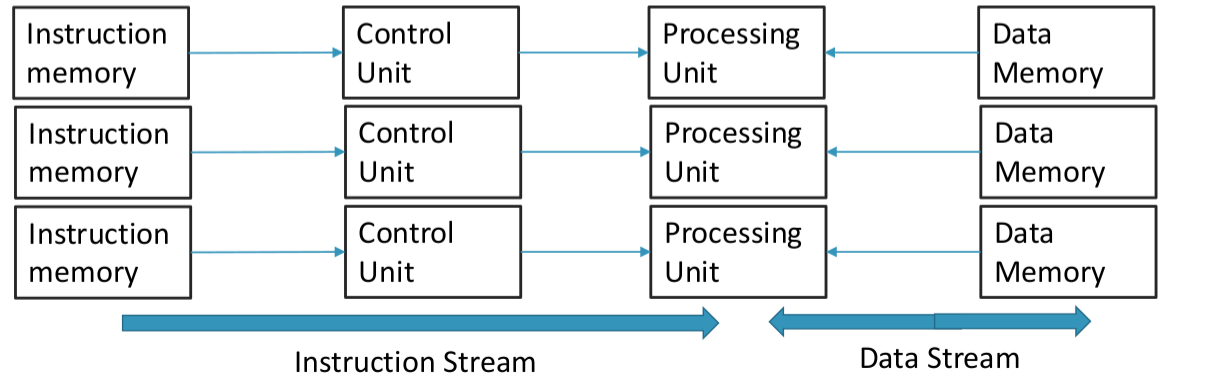
\includegraphics[width=.9\textwidth]{figure_parallel/mimd.png}
\end{subfigure}%
\begin{subfigure}{.3\textwidth}
  \centering
  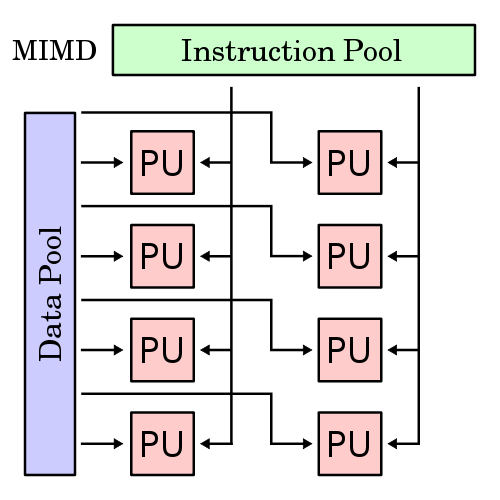
\includegraphics[width=.9\textwidth]{figure_parallel/mimd2.png}
\end{subfigure}
\end{figure}

\subsection{MISD: Multiple Instruction Single Data}
Not commonly seen. Sometime the systolic array is seen as MISD.\\
Usually is an architecture used for fault tollerance and not for computing.


\begin{figure}[ht]
\centering
\begin{subfigure}{.7\textwidth}
  \centering
  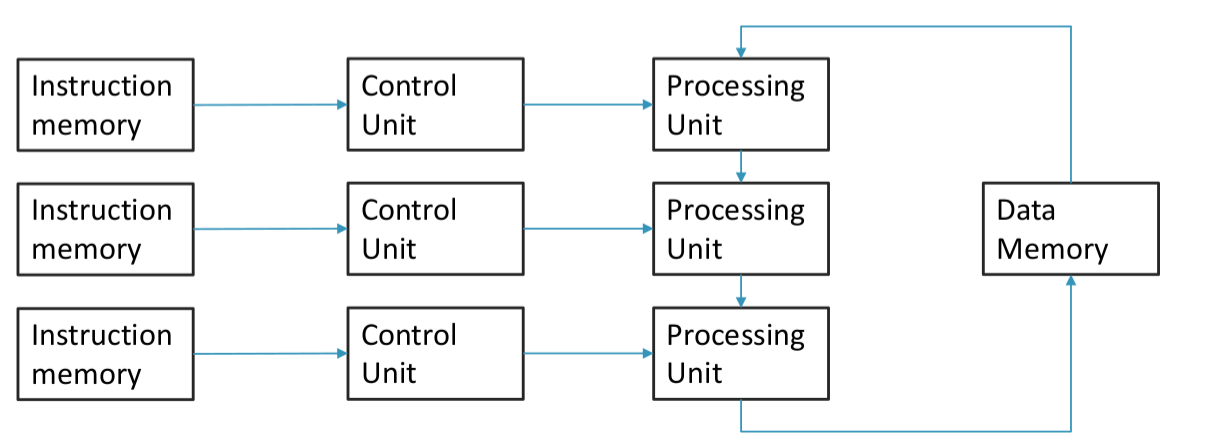
\includegraphics[width=.9\textwidth]{figure_parallel/misd.png}
\end{subfigure}%
\begin{subfigure}{.3\textwidth}
  \centering
  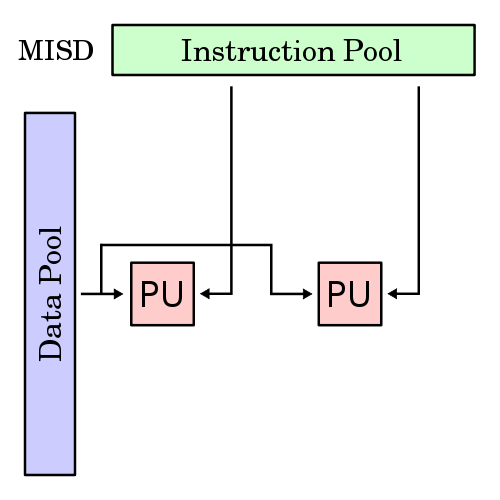
\includegraphics[width=.9\textwidth]{figure_parallel/misd2.png}
\end{subfigure}
\end{figure}

\subsection{Logic partitioning and decomposition}

\begin{wrapfigure}{r}{0.4\textwidth}
  \begin{center}
    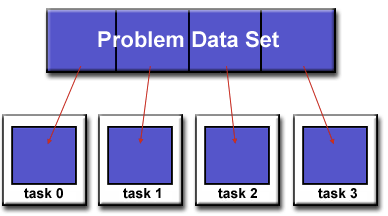
\includegraphics[width=0.35\textwidth]{figure_parallel/decomposition1.png}
    \vspace{5mm}
    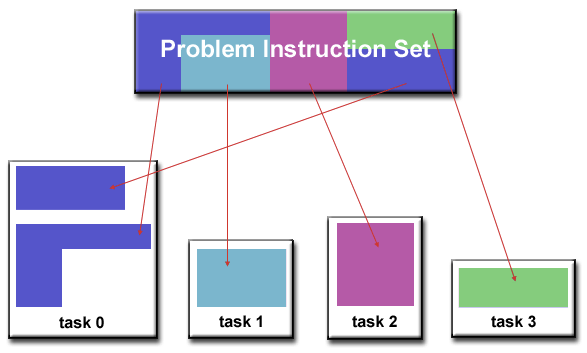
\includegraphics[width=0.35\textwidth]{figure_parallel/decomposition2.png}
  \end{center}
\end{wrapfigure}


The choice of the architecture depends on the problem.
\begin{itemize}
    \item Domain decomposition
    \begin{itemize}
        \item Single program, multiple data
        \item decomposition based on Input domain, output domain, both
    \end{itemize}
    \item Functional decomposition
        \begin{itemize}
        \item Multiple programs, multiple data
        \item Independent tasks
        \item Pipeling
    \end{itemize}
\end{itemize}

Ad esempio, se devo fare il prodotto tra matrici, divido le matrici in blocchi e faccio il prodotto.

\subsection{Multiprocessor Execution Model}
A specific architecture is suitable for a specific problem, but all needs «multiprocessors». Examples:
\begin{itemize}
    \item Each processor has its own PC and executes an independent stream of instructions (MIMD)
    \item Different processors can access the same memory space
    \item Processors can communicate via shared memory by storing/loading to/from common locations
\end{itemize}

\noindent
Two ways to use a multiprocessor:

\begin{itemize}
    \item Deliver high throughput for independent jobs via job-level parallelism
    \item Improve the run time of a single program that has been specially designed to run on a multiprocessor - a parallel-processing program
\end{itemize}


\subsection{Sequential processing}

Only one “thread” of execution:\\
-One step follows another in sequence\\
-One processor is all that is needed to run the algorithm\\

\textbf{Thread definition:} It is the smallest of a program that can be managed independently by a scheduler (typically in the operating system).\\

\noindent
- A thread is a component of a process\\
- Multiple threads can exist within one process\\
- Systems with a single processor generally implement multithreading by time slicing (software threads)


\begin{figure}[ht]
    \centering
    
\includegraphics[width=0.7\textwidth]{figure_parallel/ant_sequential.png}\end{figure}
\FloatBarrier

\subsection{Concurrent Processing}

A system in which:\\
-Multiple tasks can be executed at the same time\\
-The tasks may be duplicates of each other, or distinct tasks\\
-The overall time to perform the series of tasks is reduced\\

\noindent
\textbf{Advantages:}\\
-Concurrent processes can reduce duplication.\\
-The overall runtime of the algorithm can be significantly reduced.\\
-More real-world problems can be solved than with sequential algorithms alone.\\

\noindent
\textbf{Disadvantages}\\
-Runtime is not always reduced, so careful planning is require\\
-Concurrent algorithms can be more complex than sequential algorithms\\
-Shared data can be corrupted\\
-Communication between tasks is needed\\


\begin{figure}[ht]
    \centering
    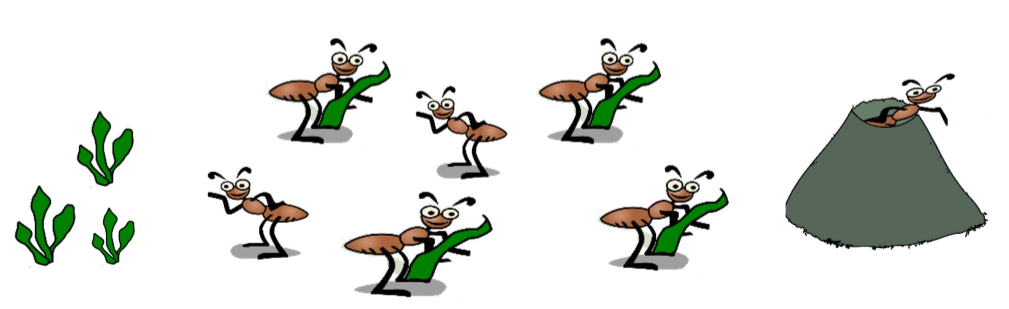
\includegraphics[width=0.7\textwidth]{figure_parallel/ant_concurrent.png}\end{figure}
\FloatBarrier

\newpage

\begin{wrapfigure}{r}{0.4\textwidth}
  \begin{center}
    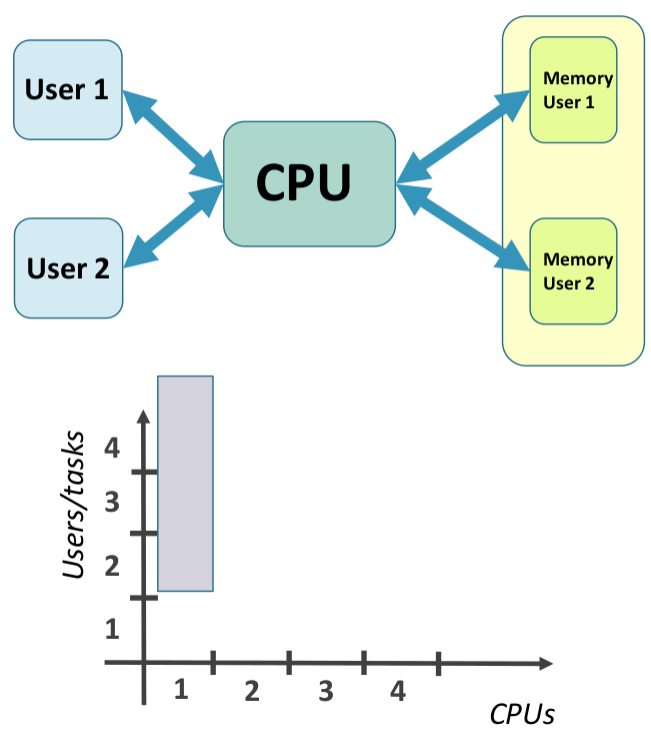
\includegraphics[width=0.38\textwidth]{figure_parallel/multiprogramming.png}
  \end{center}
  \caption{Multiprogramming \label{multiprog}}
\begin{center}
    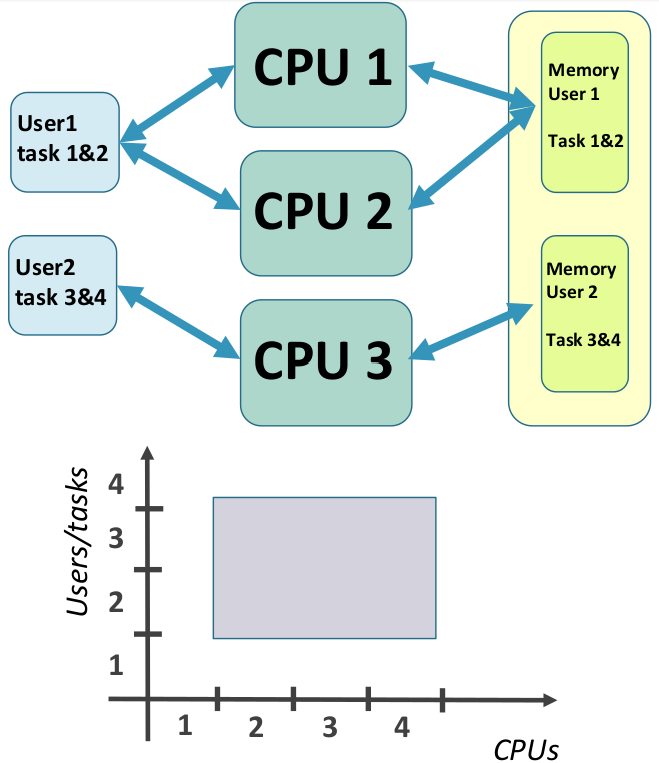
\includegraphics[width=0.38\textwidth]{figure_parallel/multiprocessing.png}
  \end{center}
  \caption{Multiprocessing \label{multiproc}}
\end{wrapfigure}

\subsection{Types of concurrent processing:}
-Multiprogramming\\
-Multiprocessing\\
-Multitasking\\
-Distributed Systems\\

\subsection{Multiprogramming}





-Share a single CPU among many users or tasks.\\
-May have a time-shared algorithm or a priority algorithm for determining which task to run next\\
-Gives the illusion of simultaneous processing through rapid swapping of tasks (interleaving).

\subsection{Multiprocessing}

-Executes multiple tasks at the same time\\
-Uses multiple processors to accomplish the tasks\\
-Each processor may also timeshare among several tasks\\
-Has a shared memory that is
used by all the tasks

\subsection{Multitasking}

-A single user can have
multiple tasks running at the
same time.\\
-Can be done with one or
more processors.\\
-Used to be rare and for only
expensive multiprocessing
systems, but now most
modern operating systems
can do it.\\

\subsection{Distributed systems}

-Multiple computers
working together with no
central program “in
charge.”\\
-No bottlenecks from
sharing processors\\
-No central point of failure\\
-Complexity\\
-Communication overhead\\
-Distributed control\\


\begin{figure}[ht]
\centering
\begin{subfigure}{.5\textwidth}
  \centering
  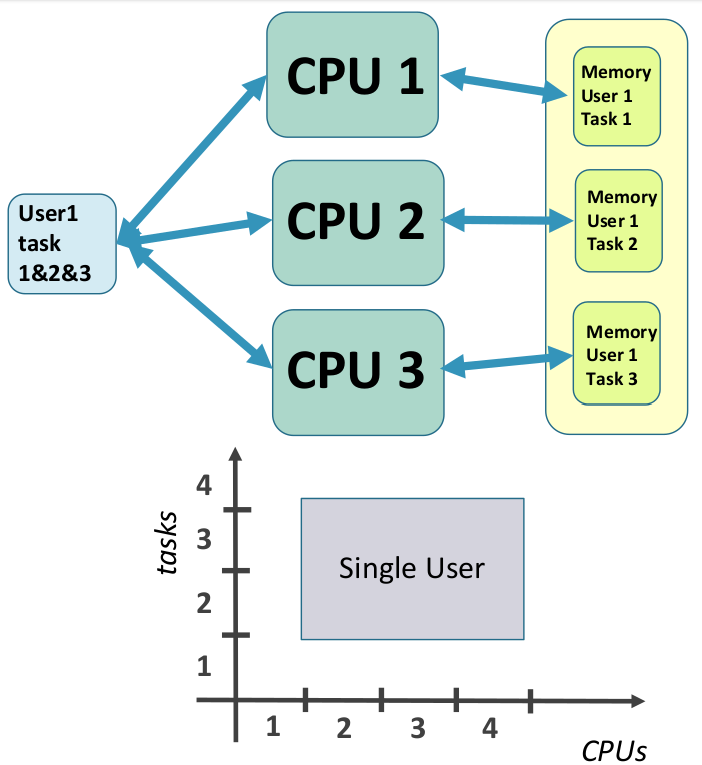
\includegraphics[width=.7\textwidth]{figure_parallel/multitasking.png}
  \caption{Multitasking}
\end{subfigure}%
\begin{subfigure}{.5\textwidth}
  \centering
  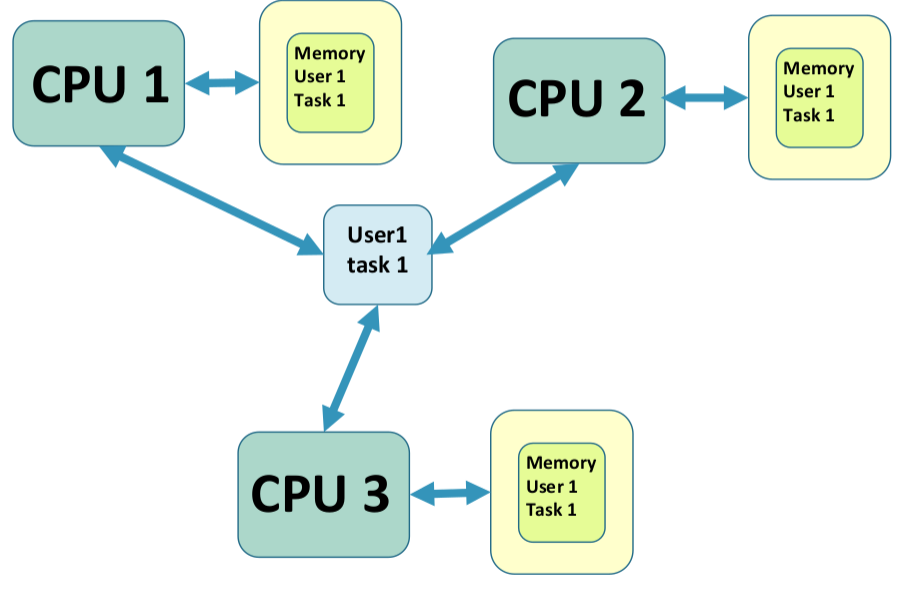
\includegraphics[width=.9\textwidth]{figure_parallel/distributed_system.png}
  \caption{Distributed Systems}
\end{subfigure}
\end{figure}

\newpage
\clearpage

\subsection{Parallelism vs Concurrency}

\textbf{Concurrency} is the execution of multiple tasks at the same time, regardless
of the number of processors.\\
\textbf{Parallelism} is the execution on multiple processors on the same task:
-Breaking the task into meaningful pieces\\
-Doing the work on many processors\\
-Coordinating and putting the pieces back together.


\begin{figure}[ht]
    \centering
    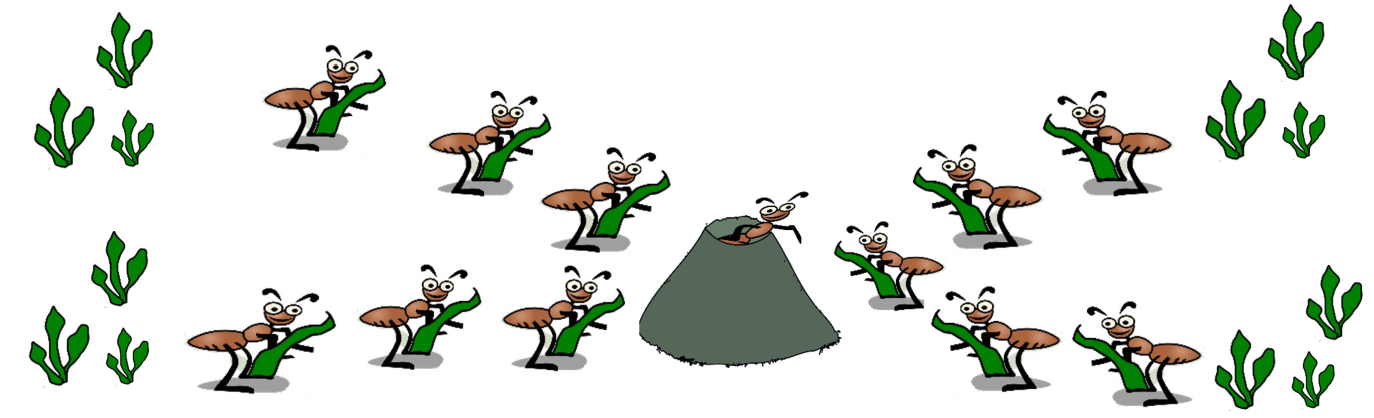
\includegraphics[width=0.7\textwidth]{figure_parallel/ant_parallelism.png}\end{figure}
\FloatBarrier


\subsection{Parallelization}

\begin{wrapfigure}{r}{0.4\textwidth}
  \begin{center}
    \includegraphics[width=0.38\textwidth]{figure_parallel/parallelization.png}
  \end{center}
\end{wrapfigure}

For a wide class of algorithms parallelization is the most powerfull way to decrease execution time (not complexity).\\
-Example: a problem with O(NlogN) complexity (for
instance Quicksort) on logN processors will take the
time needed by O(N) algorithms\\
-Example: a problem with O(N$^2$) complexity (for
instance binary search) on N processors will take the
time needed by O(N) algorithms\\

\noindent
\textbf{Parallelization is not free}. Processors must be controlled and coordinated. We need a way to govern which processor does what
work; this involves extra work.\\

Often the program must be written in a special programming language for parallel systems.
Often, a parallelized program for one machine (with, say, 2K processors) is not optimal on other machines (with, say, 2L processors).


\subsection{Speedup and Efficiency}

\begin{wrapfigure}{r}{0.4\textwidth}
  \begin{center}
    \includegraphics[width=0.38\textwidth]{figure_parallel/speedup.png}
  \end{center}
\end{wrapfigure}

How much gain can we get from
parallelizing an algorithm?\\
Let’s define the «speedup» as (where
n is the number of processors):

\begin{equation*}
    S_n = T_{serial}/T_{parallel}(n)
\end{equation*}

For a perfect parallel algorithm $S_n = n$. That's pratically impossible, even if for very specific cases could be also $S_n > n$ (superlinear case).\\

The efficiency is defined as:
\begin{equation}
    E = S_n/n
\end{equation}
It is a measure of how well our algorithm is using the processors.

\subsection{Cost and Scalability}

\textbf{Cost}: the number of CPU required
\begin{equation*}
    c = n T_p(n) = \dfrac{T_1}{E}
\end{equation*}

\textbf{Scalability}: capability to remain efficient with the increasing of the number of processors.

\subsection{Amdhal’s law (1967)}

\begin{wrapfigure}{r}{0.5\textwidth}
  \begin{center}
    \includegraphics[width=0.48\textwidth]{figure_parallel/amdahl.png}
  \end{center}
\end{wrapfigure}

If only one part ($P_K$) of the code can be improved, the maximum improvement is given by:

\begin{equation*}
    1/\sum\dfrac{P_K}{S_K}
\end{equation*}

Where k is the part of the code and $S_k$ is the speedup of the part-k.\\

In the case of parallel programming:

\begin{equation*}
    S_n = \dfrac{n}{nF + (1-F)}
\end{equation*}

if $n \longrightarrow \infty$ the speedup is $S_n = 1/F$\\
For instance if the fraction of serial code is 10\% (F=0.10) the maximum speedup is «only» 10 (regardless the number of processors).\\
Apparently the parallelism is usefull only for «embarassingly parallel» problems, with a small number of processors.



\subsection{Overhead of parallelization}

\textbf{Load balancing}\\
In case of several tasks in parallel the execution time of each task must be similar. Otherwise the total time is dominated by the slower task.\\
Some processor could be inefficently IDLE. It’s not easy to design a priori a good load balancing.\\

\textbf{Synchronization}\\
If the tasks use the same memory (shared memory) to exchange data a logic of lock-unlock must be designed. This involves a waste of time.\\

\textbf{Comunication latency}\\
If data must be moved between processors the overhead due to data transmission can be really relevant.

\subsection{Limits of Amdhal’s law}
Apparently the Amdahl’s law puts important limits to the advantages of parallel computing. But there are importants caveat to this law:

-Amdahl assumes that the best solution is always the best serial
algorithm. Often some problem must be solved in parallel\\
-Some architectural design can help parallel processing (for instance
the caching)\\
-Amdahl assumes that the dimension of the problem is always the
same with the increasing of the number of processors. But more
processors often means that wider problem can be addressed.

\subsection{Gustafson’s law (1988)}
Let’s assume s is the time of the serial part (and p is the time parallel part).\\
Let’s assume that the problem grows with the number of processor (N) and that the serial part remains always the same.\\
Under these assumptions the speedup is given by:

\begin{equation*}
    s_n = N + (1-N)s
\end{equation*}

The speedup is linear with N.


\begin{figure}[ht]
\centering
\begin{subfigure}{.5\textwidth}
  \centering
  \includegraphics[width=.9\textwidth]{figure_parallel/gustafson1.png}
\end{subfigure}%
\begin{subfigure}{.5\textwidth}
  \centering
  \includegraphics[width=.9\textwidth]{figure_parallel/gustafson2.png}
\end{subfigure}
\end{figure}

\vfill

\begin{tcolorbox}[width=\textwidth,colback={white},title={Recap: },colbacktitle=cyan,coltitle=black]

Standard processors are designed for “sequential” programming\\

-Several “tricks” are applied at instruction level to better exploit the Von Neuman structure (Vector processors, superscalars, pipeline, ...)\\

-Starting from about 2005 the performances serial processors start to show saturation (Moore’s law, Denard’s scaling)\\

-To overcome these limitations it is necessary to rethink the way of programming (Concurrency \& Parallelism)\\

-The idea: divide the problem in sub-problems to be addressed simultaneously (different architectures for parallelism: Flynn’s taxonomy)
\end{tcolorbox}


\newpage

\section{Multithreading and  multiprocessing in Python}

\subsection{Threads and processes}
Threads and processes are the way to use concurrency in python.\\ Python implements a very simple thread-safe mechanism: Global Interpreter Lock (GIL). In order to prevent conflicts only one statement in one thread is executed at a time (single-threading).\\


\begin{figure}[ht]
    \centering
    \includegraphics[width=0.6\textwidth]{figure_parallel/Thread_and_processes.png}\end{figure}
\FloatBarrier

\subsection{The Global Interpreter Lock (GIL)}

The Global Interpreter Lock refers to the fact that the Python interpreter is not thread safe. There is a global lock that the current thread holds to safely access Python objects. Because only one thread can acquire Python Objects/C API, the interpreter regularly releases and reacquires the lock every 100 bytecode of instructions. The frequency at which the interpreter checks for thread switching is controlled by the
\texttt{sys.setcheckinterval()} function. In addition, the lock is released and reacquired around potentially blocking I/O operations.\\
It is important to note that, because of the GIL, the CPU-bound applications won't be helped by threads. In Python, it is recommended to either use processes, or create a mixture of processes and threads. \\

\subsection{Processi e Thread}
Il processo è un'istanza del programma che abbiamo scritto. Ogni processo ha una memoria dedicata.\\
Quando due processi vengono lanciati, le due memorie non si parlano tra loro, sono completamente separate. Ogni processo ha una memoria chiusa.\\

All'interno di un singolo processo possiamo creare task differenti. Queste task possono essere viste come parti diverse del programma eseguite in modo seriale (ad es quando definiamo più funzioni che fanno compiti differenti per rendere più leggibile il programma).\\
Possiamo rendere questi task dei \textit{thread}: pezzi di codice che runna indipendentemente dagli altri.\\
C'è una memoria comune che è la memoria del processo. Poi ci sono thread diversi che runnano su risorse differenti (o sulla stessa risorsa) contemporaneamente.\\

Qualche volta è necessario che questi thread che stanno lavorando insieme, comunichino tra di loro. Magari vogliono leggere o scrivere qualcosa sulla memoria condivisa.Serve un meccanismo di comunicazione tra i vari thread. In che modo farli comunicare dipende da noi.\\


Il sistema operativo mette a disposizione due modi per mettere in comunicazione i thread, cercando di evitare possibili conflitti.
\textbf{Mutex}: è un sistema di locking: quando un thread vuole accedere a una parte di memoria o a una risorsa hardware, dice "questo lo sto usando io" e gli altri thread devono mettersi in coda fino a quando il lock non viene sganciato.\\
\textbf{Meccanismo dei Semafori}: si basa sul fatto che un thread comunichi agli altri thread cosa sta facendo. Nel caso del Mutex vince chi mette il lock e solo lui può toglierlo. Nel caso del semaforo c'è un meccanismo di priorità logica che permette a qualcun altro di prendere in mano la risorsa.\\

Python non permette di fare thread! Python è un linguaggio pensato per essere semplice, nel senso che impedisce di fare troppe cavolate.\\
Python è un linguaggio fortemente tipizzato. Non dichiaro mai le variabili, ma dopo che faccio \texttt{a = 1}, da quel punto la variabile è un intero e non posso cambiarlo, non posso successivamente scrivere \texttt{a = 1.5}.\\
\noindent
GIL = Global Interpreter Lock. Si possono definire i thread, ma fisicamente non vengono runnati insieme, bensì in modo seriale.
Allora perché farlo?\\
I thread sono utili quando è necessario fare I/O.\\
Se ho un thread che deve accedere a un file, python me lo permette.\\

Se voglio fare roba concorrenziale di \textbf{calcolo} contemporaneamente? Dobbiamo utilizzare i \textit{processi}: istanze di programmi.\\

Posso dire che tre funzioni all'interno di un programma vengano fatte in processi differenti, che effettivamente runneranno in parallelo. Questo ha lo svantaggio che i processi abbiano memorie differenti, quindi devo trovare un modo per farle comunicare.
Ho però il vantaggio di poter uccidere (kill) un singolo processo.\\

C'è un altro modo per fregare GIL, ovvero non usare python. Ad esempio quando usiamo alcune librerie, wrappate in python, ma scritte in C. E quelle librerie al loro interno usano i thread!\\

\textit{controllare di avere i moduli "multiprocessing" e "threading"}

\begin{tcolorbox}[width=\textwidth,colback={white},title={Process: pros and cons},colbacktitle=cyan,coltitle=black]
\textbf{pros:}\\
-A process is an instance of a program, managed by operating system (memory space allocated by the kernel).\\
-Two processes can executecode simultaneously in thesame python program\\
-Separated memory space\\
-Takes advantage of multiple cores and CPUs\\
-Child processes are killable\\
-Avoid GIL limitations\\
\textbf{cons:}\\
-Relatively high overhead\\
-Open and close processes takes more time\\
-Sharing information between processes is very slow\\
-Model not adaptable to parallelism
\end{tcolorbox}


\begin{tcolorbox}[width=\textwidth,colback={white},title={Threads: pros and cons},colbacktitle=green,coltitle=black]
\textbf{pros:}\\
-Processes produce threads (sub-processes) to handle sub-tasks (threads live inside the process and share the same memory space)\\

-Can use shared memory\\
-Threads communication\\
-Lightweight\\
-Very small overhead\\
-Great option for I/O bound application\\
\textbf{cons:}\\
-Subject to GIL (although there are workarounds)\\
-Not killable\\
-Potential of race condition \\
-Same memory space
\end{tcolorbox}

\subsection{When to use threads vs processes?}
\textbf{Processes} speed up Python operations that are CPU intensive because they benefit from multiple cores and avoid the GIL.\\
\textbf{Threads} are best for IO tasks or tasks involving external systems because threads can combine their work more efficiently. Processes need to pickle their results to combine them which takes time.\\

Threads provide no benefit in python for CPU intensive tasks because of the GIL.

\subsection{Things to be afraid of! (not only in python...)}

\textbf{Starvation}: a task is costantly denied necessary resource. The task can never finish (starves).\\
\textbf{Deadlock}: Usually a deadlock occurs when two or more tasks wait cyclically for each other.


\begin{figure}[ht]
    \centering
    \includegraphics[width=0.5\textwidth]{figure_parallel/deadlock.png}\end{figure}
\FloatBarrier

\newpage
\section{\textit{Lun 24 ott - Lezione 10}}

\subsection{The multiprocessing module}
\subsubsection{HelloWorld}
Create a process
to run the function
f()

\inputminted{python}{python_parallel/HelloWorld.py}



Trasformeremo quello che fa la funzione in un processo.\\
Una volta definito il processo, lo dobbiamo fare partire usando il metodo \texttt{p.start}.
L'esecuzione di un thread può avvenire in modo sincrono e asincrono. Tipicamente avviene in modo asincrono: quando l'interprete trova \texttt{p.start} avvia il processo. Il processo parte; Il controllo del flusso va direttaente alla riga successiva, indipendentemente dl fatto che il processo sia terminato.
Questo succede a meno che non utilizziamo \texttt{p.join}. In tal caso il processo avviene in modo sincrono: finché non è finito il processo, si aspetta.

\subsubsection{FatherAndSons}
Generate a tree of processes

\inputminted{python}{python_parallel/FatherAndSons.py}


Ho un processo main in cui viene chiamata la funzione f0. Il main genera un processo, definito dalla funzione f1, nel quale viene chiamata f2.\\

\begin{figure}[ht]
    \centering
    \includegraphics[width=0.5\textwidth]{figure_parallel/father_sons.png}\end{figure}
\FloatBarrier

Su linux, se sulla linea di comando scriviamo \texttt{ps}, mi dice quali processi sono in esecuzione.\\

\subsubsection{Use the Queue to get the result from multiple processes}

\inputminted{python}{python_parallel/FourProcesses.py}


La queue è una scatola in cui mettiamo dentro il risultato dei vari processi, per poi aprirla nel main.\\
\textbf{nota:} non possiamo assumere l'ordine delle cose che facciamo. Lo scheduler decide quando far partire i processi, che potrebbero finire in un ordine diverso da quello atteso.

\subsubsection{How to distribute work to
workers (aka cpu cores)}
Use the Pool class.\\
Try \texttt{Pool.map}\\
Try \texttt{Pool.map\_async}\\
See also \texttt{Pool.apply} e \texttt{Pool.apply\_async}


\begin{minted}{python}
def cube(x):
    print (str(os.getpid())+" "+str(os.getppid()))
    return x**3
#MAIN
if __name__=="__main__":
    pool = mp.Pool(processes=4)
    results = pool.map(cube,range(1,7))
    print(results)
\end{minted}

\begin{minted}{python}
#MAIN
if __name__=="__main__":
    pool = mp.Pool(processes=4)
    results = pool.map_async(cube,range(1,7))
    print(results.get())
\end{minted}

\textbf{nota} i processi avviati con pool.map sono di per sé sincroni (e partono subito), perciò non serve usare \texttt{join} (e \texttt{start}).\\

\subsubsection{Another example with \texttt{pool.map} and \texttt{pool.map\_async}}
Notice the time
measurement

\begin{minted}{python}
import multiprocessing as mp
import time
import os
def doingstuffs(x):
    print ("Process: "+str(x)+" "+str(os.getpid()))
    time.sleep(1)
if __name__=="__main__":
    start=time.time()
    pool = mp.Pool(processes=4)
    results = pool.map(doingstuffs,range(1,10))
    end=time.time()
    print("elapsed time: "+str(end-start))
\end{minted}

\begin{minted}{python}
results = pool.map_async(doingstuffs,range(1,10))
#…
print(results.get())
\end{minted}


\subsection{Communication between processes}

Un modo per (\textit{illuderci di}) passare informazione da un processo al'altro è utilizzare le variabili globali.

\inputminted{python}{python_parallel/communication1.py}



\begin{figure}[ht]
    \centering
    \includegraphics[width=0.45\textwidth]{figure_parallel/communication_global.png}\end{figure}
\FloatBarrier

Different memory spaces allocated for each process.
Try to print result in both processes.

\subsubsection{Comm. between processes: shared memory}

Normalmente abbiamo visto che le memorie sono separate. \'E possibile definire una zona di memoria (\textit{shared memory}) comune ad entrambi i processi.

\begin{figure}[ht]
    \centering
    \includegraphics[width=0.45\textwidth]{figure_parallel/shared_memory.png}\end{figure}
\FloatBarrier

Shared memory:
multiprocessing module provides Array and Value objects to share data between processes.\\
\texttt{Array:} array allocated from shared
memory.\\
\texttt{Value:} object allocated from shared
memory.

\inputminted{python}{python_parallel/communication2.py}



Nella shared memory non posso mettere oggetti complicati come i dizionari.


\subsubsection{Comm. between processes: server process}


Server process : Whenever a python program
starts, a server process is also started. From
there on, whenever a new process is needed,
the parent process connects to the server and
requests it to fork a new process.
A server process can hold Python objects and allows
other processes to manipulate them.
multiprocessing module provides a Manager class
which controls a server process. Hence, managers
provide a way to create data which can be shared
between different processes.
Server process allows to share any type of object (dict,
lists,…). It is also possible to connect a server process
to the network

\inputminted{python}{python_parallel/communication3.py}

\begin{figure}[ht]
    \centering
    \includegraphics[width=0.55\textwidth]{figure_parallel/server_process.png}\end{figure}
\FloatBarrier

\subsubsection{Comm. between processes: queue}

\textbf{Queue :} A simple way to communicate between process with multiprocessing is to use a Queue to pass messages back and forth.\\
Any Python object can pass through a Queue.

\begin{figure}[ht]
    \centering
    \includegraphics[width=0.45\textwidth]{figure_parallel/queue.png}\end{figure}
\FloatBarrier


\inputminted{python}{python_parallel/communication4.py}

\textbf{nota:} quando estraggo un elemento dalla coda, lo rimuovo da essa.


\subsubsection{Comm. between process: pipe}

In linea di principio, la coda permette di avere più \textit{endpoint}: non necessariamente entra da un lato ed esce da un altro. Invece la pipe è così: la dobbiamo immaginare proprio come un tubo.

\begin{figure}[ht]
    \centering
    \includegraphics[width=0.5\textwidth]{figure_parallel/pipe.png}\end{figure}
\FloatBarrier

Se ho soltanto due processi: uno che scrive e uno che legge, allora è più conveniente usare le pipe perché sono più veloci.\\

\textbf{Pipes :} A pipe can have only two endpoints. Hence, it is preferred over queue when only two-way communication is required. Queue is slower (it’s built on top of pipe).\\

multiprocessing module provides \texttt{Pipe()} function which returns a pair of connection objects connected by a pipe.
The two connection objects returned by \texttt{Pipe()} represent the two ends of the pipe.
Each connection object has \texttt{send()} and \texttt{recv()} methods (among others).


\subsection{Synchronization between processes}

Process synchronization is defined as a mechanism which ensures that two or more concurrent processes do not simultaneously execute some particular program segment known as critical section. A race condition occurs when two or more processes can access shared data and they try to change it at the same time. As a result, the values of variables may be unpredictable and vary depending on the timings of context switches of the processes.

\inputminted{python}{python_parallel/synchro1.py}


Se permettiamo a due processi di scrivere contemporaneamente sulla stessa locazione di memoria succede un casino!

multiprocessing module provides a Lock class to deal with the race conditions. Lock is implemented using a Semaphore object provided by the Operating System. A semaphore is a synchronization object that controls access by multiple processes to a common resource in a parallel programming environment. It is simply a value in a designated place in operating system (or kernel) storage that each process can check and then change. Depending on the value that is found, the process can use the resource or will find that it is already in use and must wait for some period before trying again.

\inputminted{python}{python_parallel/synchro2.py}

Il lock si utilizza ogni volta che si vuole impedire che la stessa risorsa venga usata due volte.


\subsection{Threading}



A thread is an entity within a process that can be scheduled for execution. Also, it is the smallest unit of processing that can be performed in an OS (Operating System).\\
In simple words, a thread is a sequence of such instructions within a program that can be executed
independently of other code. For simplicity, you can
assume that a thread is simply a subset of a
process!
Multiple threads can exist within one process where:\\
-Each thread contains its own register set and local variables (stored in stack).\\
-All thread of a process share global variables (stored in heap) and the program code.

\begin{figure}[ht]
    \centering
    \includegraphics[width=0.45\textwidth]{figure_parallel/thread.png}\end{figure}
\FloatBarrier

\subsection{Threading module}



The threads aren’t different processes. Due to GIL the parallelism is only «Logic».

\inputminted{python}{python_parallel/thread1.py}


\subsection{Threads synchronization}

\inputminted{python}{python_parallel/thread2.py}
\inputminted{python}{python_parallel/thread2b.py}


\subsection{Comparison between Threads and Processes}

Write a code to factorize a list of numbers: the 300 odd numbers from 1000000000001 and 1000000000597.\\

Try to benchmark the time needed to factorize this list by using:\\
-Serial code\\
-2,4,8 Threads\\
-2,4,8 Processes\\
Produce a plot with the results


\begin{figure}[ht]
	\centering
	\includegraphics[width=1\textwidth]{figure_parallel/comparison_thread_processes.png}\end{figure}
\FloatBarrier


\inputminted{python}{python_parallel/final_example.py}


\begin{figure}[ht]
	\centering
	\includegraphics[width=0.5\textwidth]{figure_parallel/comparison_time.png}\end{figure}
\FloatBarrier

\subsection{Why should I use threads?}
GIL is bypassed in two cases:\\
-running programs in external C code (ex: numpy)\\
-in case of I/O operation: Python release the lock waiting for I/O\\

A tipical application is the use of the network. Writing to a disk, display an image to the screen, print on a printer,…



\begin{minted}{python}
import requests
import threading as thr
from time import perf_counter

buffer_size=1024
#define a function to manage the download
def download(url):
	response = requests.get(url, stream=True)
	filename = url.split("/")[-1]
	with open(filename,"wb") as f:
		for data in response.iter_content(buffer_size):
			f.write(data)

#MAIN
if __name__ == "__main__":
	urls= [
		"http://cds.cern.ch/record/2690508/files/201909-262_01.jpg",
		"http://cds.cern.ch/record/2274473/files/05-07-2017_Calorimeters.jpg",
		"http://cds.cern.ch/record/2274473/files/08-07-2017_Spectrometer_magnet.jpg",
		"http://cds.cern.ch/record/2127067/files/_MG_3944.jpg",
		"http://cds.cern.ch/record/2274473/files/08-07-2017_Electronics.jpg",
	]

	t = perf_counter()
#sequential download
	for url in urls:
		download(url)
	print("Time: "+str(perf_counter()-t))

\end{minted}


Versione parallela: faccio 5 thread che scaricano contemporaneamente 5 immagini:

\begin{minted}{python}

import threading as thr
import requests
import os
from time import perf_counter

buffer_size=1024

#define a function to manage the download
def download(url):
	response = requests.get(url, stream=True)
	filename = url.split("/")[-1]
	with open(filename,"wb") as f:
		for data in response.iter_content(buffer_size):
			f.write(data)
			
			
#MAIN
if __name__ == "__main__":
	urls= [
		"http://cds.cern.ch/record/2690508/files/201909-262_01.jpg",
		"http://cds.cern.ch/record/2274473/files/05-07-2017_Calorimeters.jpg",
		"http://cds.cern.ch/record/2274473/files/08-07-2017_Spectrometer_magnet.jpg",
		"http://cds.cern.ch/record/2127067/files/_MG_3944.jpg",
		"http://cds.cern.ch/record/2274473/files/08-07-2017_Electronics.jpg",
	]
	
#define 5 threads
	threads = [thr.Thread(target=download, args=(urls[x],)) for x in range(4)]

	t = perf_counter()
	
#start threads
	for thread in threads:
		thread.start()
		
#join threads
	for thread in threads:
		thread.join()
		
	print("Time: "+str(perf_counter()-t))
\end{minted}

Performaces depend on network speed. Overheads for thread start and lock release.


\subsection{Process vs Threads}

\begin{figure}[ht]
    \centering
    \includegraphics[width=0.7\textwidth]{figure_parallel/process_vs_thread.png}\end{figure}
\FloatBarrier



\newpage
\section{\textit{Gio 27 ottobre - Lezione 11}}
\section{Introduction to GPU computing (1)}

\subsubsection{Moore's Law}

Moore’s law: “The performance of microprocessors and the number of their transistors will double every 18 months”.\\
The increasing of performance is related to the clock.\\
Faster clock means higher dissipation $\rightarrow$ power wall

\begin{figure}[ht]
	\centering
	\includegraphics[width=0.5\textwidth]{figure_parallel/moore.png}\end{figure}
\FloatBarrier


\subsection{Parallel programming}

Parallel computing is no longer something for SuperComputers. All the processors nowadays are multicores.\\
The use of parallel architectures is mainly due to the physical constraints to
frequency scaling.

\begin{figure}[ht]
	\centering
	\includegraphics[width=0.5\textwidth]{figure_parallel/parallel_programming.png}\end{figure}
\FloatBarrier

\subsection{Limits of parallel programming}

Several problems can be split in
smaller problems to be solved
concurrently. In any case the maximum speedup is not linear , but it depends on the serial part of the code (Amdahls’s law)\\
The situation can improve if the
amount of parallelizable part
depends on the resources(Gustafson’s Law)

\begin{figure}[ht]
	\centering
	\includegraphics[width=0.5\textwidth]{figure_parallel/limits_parallel_programming.png}\end{figure}
\FloatBarrier

\begin{equation*}
	S_{latency} = \dfrac{1}{1-p+\frac{p}{s}}
\end{equation*}

\begin{equation*}
	S_{latency} = 1 - p + sp
\end{equation*}

\subsection{What are GPUs?}

The GPUs are processors dedicated to parallel programming for
graphical application.
Rendering, Image transformation, ray tracing, etc. are typical
application where parallelization can helps a lot.


\subsection{Standard GPU pipeline}

\begin{figure}[ht]
	\centering
	\includegraphics[width=1\textwidth]{figure_parallel/gpu_pipeline.png}\end{figure}
\FloatBarrier

Ogni triangolino è indipendente dall'altro. Possiamo agire contemporaneamente su questi triangolini in maniera parallela.

\subsection{Standard GPU requirements}

\textbf{Graphics pipeline}: huge amount of arithmetic on independent data:\\
-Transforming positions\\
-Generating pixel colors\\
-Applying material properties and light situation to every pixel\\
\textbf{Hardware needs}\\
-Access memory simultaneously and contiguously\\
-Bandwidth more important than latency\\
-Floating point and fixed-function logic\\

\subsection{What are the GPUs?}

The technical definition of a GPU is "a single-chip processor with integrated
transform, lighting, triangle setup/clipping, and rendering engines that is
capable of processing a minimum of 10 million polygons per second.“\\
The possibility to use the GPU for generic computing (GPGPU) has been
introduced by NVIDIA in 2007 (CUDA)\\
In 2008 OpenCL: consortium of different firms to introduce a multi-platform
language for manycores computing.

\subsection{Why the GPUs?}

-GPU is a way to cheat the Moore’s law\\
Implementano la possibilità di eseguire operazioni ad una velocità superiore a quella del clock.\\
-SIMD/SIMT parallel architecture\\
-The PC no longer get faster, just wider.\\
-Very high computing power for «vectorizable» problems\\
-Impressive derivative almost a factor of 2 in each generation\\
-Continuous development\\
-Easy to have a desktop PC with teraflops of computing power, with thousand of cores.\\
-Several applications in HPC, simulation, scientific computing…\\

Vogliamo imparare a sfruttare una tecnologia utilizzata sul mercato (che migliora ogni anno), per i nostri scopi di calcolo scientifico.\\

\subsection{A lot of cores...}

\begin{figure}[ht]
	\centering
	\includegraphics[width=0.5\textwidth]{figure_parallel/cores.png}\end{figure}
\FloatBarrier


\begin{figure}[ht]
	\centering
	\includegraphics[width=0.5\textwidth]{figure_parallel/cores2.png}\end{figure}
\FloatBarrier


\subsection{Metrics}

\textbf{FLOPS} (Floating Point operation per
second):\\
It is a measurement of the computing power of a processor. Theoretically is defined as:
\begin{equation*}
	FLOPS = clock * cores * Operation/cycle
\end{equation*}
%%%%
Actually this formula doesn’t take into account several things\\
The real extimation is made experimentally by using standard packages (LINPACK,
LAPACK)\\
The FLOPS is only a first indication of the computing power.\\
Other metrics has been invented to avoid the limitations of the FLOPS.\\

\textbf{SPECint and SPECf}\\
They are suites of 12 benchmarks of different type (for integer and floating point). The extimation is relative to a particular
machine.



\begin{figure}[ht]
\centering
\begin{subfigure}{.5\textwidth}
	\centering
	\includegraphics[width=.9\linewidth]{figure_parallel/metrics.png}
\end{subfigure}%
\begin{subfigure}{.5\textwidth}
	\centering
	\includegraphics[width=.9\linewidth]{figure_parallel/metrics2.png}
\end{subfigure}
\end{figure}
\FloatBarrier







\subsection{Computing power comparison}

\begin{figure}[ht]
	\centering
	\includegraphics[width=0.9\textwidth]{figure_parallel/computing_power_comparison.png}\end{figure}
\FloatBarrier

\subsection{CPU}

-\textbf{Multilevel and Large Caches}: Convert long latency memory access to -short latency cache latency.\\
-\textbf{Branch prediction:} To reduce latency in branching
-Instruction level parallelism (ILP)\\
-Powerful ALU: Reduced operation latency\\
-Memory management\\
-Large control part\\

\begin{figure}[ht]
	\centering
	\includegraphics[width=0.38\textwidth]{figure_parallel/CPU.png}
	\caption{CPU: latency oriented design}
\end{figure}
\FloatBarrier

\subsection{GPU}

-SIMT/SIMD (Single instruction Multiple Thread/Data) architecture\\
-SMX (Streaming Multi Processors) to execute kernels\\
-Thread level parallelism: Massive threading to hide the latency\\
-Limited caching: To boost memory throughput\\
-Limited control\\
-No branch prediction, but branch predication

\begin{figure}[ht]
	\centering
	\includegraphics[width=0.36\textwidth]{figure_parallel/GPU.png}
	\caption{GPU: throughput oriented design}
\end{figure}
\FloatBarrier

\subsection{CPU vs GPU}

\begin{figure}[ht]
	\centering
	\includegraphics[width=1\textwidth]{figure_parallel/cpu_vs_gpu.png}
\end{figure}
\FloatBarrier


\begin{figure}[ht]
	\centering
	\includegraphics[width=0.8\textwidth]{figure_parallel/cpu_vs_gpu_table.png}
\end{figure}
\FloatBarrier

\subsection{SIMT}


\begin{wrapfigure}{r}{0.45\textwidth}
	\begin{center}
		\includegraphics[width=0.43\textwidth]{figure_parallel/simt.png}
	\end{center}
\end{wrapfigure}

Consideriamo un processore da 4000 core. La struttura SIMD prevederebbe che tutti i core facciano la stessa cosa nello stesso momento (ad es sommare due vettori di 4000 elementi).



\begin{itemize}
	\item Standard CPU : Scalar processors
	\item SIMD CPU: vector processors
	\item Simultaneous threads in multicore processors
	\item SIMT (Single Instruction Multiple	Threads)
	\begin{itemize}
		\item CPU core ~ GPU multiprocessor (SMX)
		\item Working unit: a set of threads (32, a warp)
		\item Fast switching of threads
	\end{itemize}
\end{itemize}

\subsection{CPU core vs GPU SMX}

\begin{figure}[ht]
	\centering
	\includegraphics[width=1\textwidth]{figure_parallel/core_vs_smx.png}
\end{figure}
\FloatBarrier


The latency in a SMX is hidden thanks to very deep pipelines.\\
The multithreading in a single CPU core is based on context switching.\\



\subsection{GPU+CPU}

\begin{wrapfigure}{r}{0.5\textwidth}
	\begin{center}
		\includegraphics[width=0.3\textwidth]{figure_parallel/GPU_CPU.png}
	\end{center}
\end{wrapfigure}

The winning application uses both CPU and GPU:

\begin{itemize}
	\item CPUs for sequential parts
	\begin{itemize}
		\item can be 10X faster than GPU for sequential code
	\end{itemize}
	\item GPUs for parallel part where throughput wins
	\begin{itemize}
		\item can be 100X faster than CPU for parallel code
	\end{itemize}
	\item The Host-Device connection is done with PCIe-gen3 (16 GB/s) or NVLINK (80 GB/s)
	\begin{itemize}
		\item Relatively slow
		\item Do as little as possible
	\end{itemize}
	\item The bandwidth between GPU and video memory is HBM2 (720 GB/s in P100, 900 GB/s in V100)
\end{itemize}


\vfill

\begin{tcolorbox}[width=\textwidth,colback={white},title={Summary: },colbacktitle=cyan,coltitle=black]
	\begin{itemize}
		\item Superscalars, Pipelining and Vectorialization are methods to exploit some «parallelism» at the instruction and data level: ILP
		\begin{itemize}
			\item Probably OOO (Out-of-order) execution should be included in this category
		\end{itemize}
		\item The possible improvement thanks to ILP depends on problem and data structures
		\begin{itemize}
			\item 1x-10x for Superscalars and Pipeline
			\item 2x,4x,8x,16x for the vectorialization
		\end{itemize}
		\item These methods show «saturation» because they are limited by the CPU resources available
		\begin{itemize}
			\item Pentium 4: 30 pipeline stages (nowadays 10-15 maximum)
			\item ARM A57 (Apple A7/A8): 9 ports/6 instructions superscalar
			\item Intel Tiger Lake: vector of 512 bits for a subset of AVX512 instructions
		\end{itemize}
	\end{itemize}  
	… the point is: can CPU resources grow indefinitely?
\end{tcolorbox}

\newpage
\clearpage

\section{Introduction to GPU computing (2)}
\subsection{CUDA model}


\begin{figure}[ht]
	\centering
	\includegraphics[width=0.4\textwidth]{figure_parallel/cuda.png}
\end{figure}
\FloatBarrier

CUDA is a set of C/C++ extensions to enable the GPGPU computing on
NVIDIA GPUs. Dedicated APIs allow to control almost all the functions of the graphics processor.\\
Three steps:
\begin{enumerate}
	\item copy data from Host to Device
	\item copy Kernel and execute
	\item copy back results
\end{enumerate}

\subsection{Grid, blocks and threads}

The computing resources are logically (and physically) grouped in a flexible parallel model of computation:\\
\begin{itemize}
	\item 1D,2D and 3D grid
	\item With 1D, 2D and 3D blocks
	\item With 1D, 2D and 3D threads
\end{itemize}

Only threads can communicate and synchronize in a block.\\
Threads in different blocks do not interact, threads in same block execute same instruction at the same time.\\
The “shape” of the system is decided at kernel launch time.

\begin{figure}[ht]
	\centering
	\includegraphics[width=0.55\textwidth]{figure_parallel/gbt.png}
\end{figure}
\FloatBarrier

\subsection{GPU structure}
I singoli thread runnano sui core.
I thread sono raggruppate in blocchi. Un blocco è implementato da un multiprocessore.

\begin{figure}[ht]
	\centering
	\includegraphics[width=0.7\textwidth]{figure_parallel/gpu_structure.png}
\end{figure}
\FloatBarrier

\subsection{Multiprocessor}
Anche se il numero di core è più piccolo del numero di thread, continua a poterli runnare, perché lo scheduler si prende il compito di fare eseguire i vari compiti in maniera parallela.

\begin{figure}[ht]
	\centering
	\includegraphics[width=0.5\textwidth]{figure_parallel/multiprocessor.png}
\end{figure}
\FloatBarrier

\subsection{Memory}

The memory hierarchy is fundamental in GPU programming.
Most of the memory managing and data locality is left to the user.\\
\begin{itemize}
	\item Unified Address Space
	\item Global Memory
	\begin{itemize}
		\item On board, relatively slow, lifetime of the application, accessible from host and device 
	\end{itemize}
	\item Shared memory/registers
		\begin{itemize}
		\item On Chip, very fast, lifetime of blocks/threads, accessible from kernel only
	\end{itemize}
\end{itemize}



\begin{figure}[ht]
	\centering
	\includegraphics[width=0.7\textwidth]{figure_parallel/memory.png}
\end{figure}
\FloatBarrier

\subsection{Asynchronicity}

\textbf{Problem}: Memory transfer is comparably slow\\
\textbf{Solution}: Do something else in meantime (computation)!\\
Overlap tasks:\\
-Copy and compute engines run separately (streams)
-GPU needs to be fed: Schedule many computations
-CPU can do other work while GPU computes; synchronization


\begin{figure}[ht]
	\centering
	\includegraphics[width=0.5\textwidth]{figure_parallel/asyncronicity.png}
\end{figure}
\FloatBarrier


\subsection{How to program GPU?}

\begin{itemize}
	\item CUDA is the “best” way to program NVIDIA GPU at “low level”
	\item If your code is almost CPU or if you need to accelerate dedicated functions, you could consider to use
	\begin{itemize}
		\item Directives
			\begin{itemize}
			\item OpenMP, OpenACC, …
			\end{itemize}
	\end{itemize}
		\begin{itemize}
		\item Libraries
			\begin{itemize}
			\item Thrust, ArrayFire,…
			\end{itemize}
		\end{itemize}
	\item OpenCL is a framework equivalent to CUDA to program multiplatforms
	\begin{itemize}
		\item GPU, CPU, DSP, FPGA,… 
	\end{itemize}
	\item C/C++ and Fortran are the “official” languages for CUDA
		\begin{itemize}
		\item Python and other languages are supported through	wrapping and libraries
		\end{itemize}
	\end{itemize}

\subsection{Libraries: cuBLAS}

GPU-parallel linear algebra routines (152 routines).\\
Single, double, complex data types\\
Possibility to use multiple GPUs\\
Example (among 152 routines): Saxpy: given two vectors x[10] and y[10] compute y[i]=a*x[i]+y[i]\\
\url{https://docs.nvidia.com/cuda/cublas/index.html}\\
\url{https://developer.nvidia.com/cublas}\\

\begin{minted}{c}
int a = 42;
int n = 10;
float x[n], y[n];
// fill x, y
cublasInit();
float * d_x, * d_y;
cudaMalloc((void **)&d_x, n * sizeof(x[0]);
cudaMalloc((void **)&d_y, n * sizeof(y[0]);
cublasSetVector(n, sizeof(x[0]), x, 1, d_x, 1);
cublasSetVector(n, sizeof(y[0]), y, 1, d_y, 1);
cublasSaxpy(n, a, d_x, 1, d_y, 1);
cublasGetVector(n, sizeof(y[0]), d_y, 1, y, 1);
cublasShutdown();
\end{minted}

\subsection{Libraries: Thrust}

-Template library\\
-Data parallel primitives (scan(), sort(), reduce(), … )\\
-Comes when you install CUDA for free\\

\begin{minted}{c}
int a = 42;
int n = 10;
thrust::host_vector<float> x(n), y(n);
// fill x, y
thrust::device_vector d_x = x, d_y = y;
using namespace thrust::placeholders;
thrust::transform(d_x.begin(), d_x.end(), d_y.begin(), d_y.begin(), a * _1 + _2);
x = d_x;
\end{minted}

\subsection{Directives: OpenMP, OpenACC}

The directive is the best transparent way to use GPU.\\
You must only «annotate» the part of the code you want to parallelize:
\begin{minted}{c}
#pragma acc loop
for (int i = 0; i < 100; i++) {};
\end{minted}

\subsection{Hello world}

Per compilare si usa il compilatore \texttt{nvcc}. Lo si installa installando CUDA dal sito NVIDIA.

\begin{minted}{shell}
	nvcc -o HelloWorldGpu HelloWorldGpu.cu -arch=compute_30 -code=sm_30
\end{minted}

\noindent
\textbf{Pro}: Portability; easy to program\\
\textbf{Cons}: Not all the raw GPU power available; harder to debug; easy to program wrong\\

OpenACC is more focused on GPU, while OpenMP is for multi-computers (but still usable with GPU)\\

\begin{minted}{c}
void saxpy_acc(int n, float a, float * x, float * y) {
	#pragma acc kernels
	for (int i = 0; i < n; i++) y[i] = a * x[i] + y[i];
}
…
int a = 42;
int n = 10;
float x[n], y[n];
// fill x, y
saxpy_acc(n, a, x, y);
\end{minted}

\subsection{Direct Programming: CUDA vs OpenCL}

\begin{multicols}{2}
	CUDA:
	\begin{itemize}
		\item NVIDIA GPU’s Platform
		\item Platform: Drivers, programming language (CUDA C/C++), API, compiler, debuggers, profilers, …
		\item Only NVIDIA GPUs
		\item Compilation with dedicated compiler (nvcc)
		\item CUDA fortran
	\end{itemize}
	
	\columnbreak
	
	OpenCL:
	\begin{itemize}
		\item Consortium: Open Computing Language by Khronos Group (Apple, IBM, AMD, NVIDIA, …)
		\item Programming language (OpenCL C/C++), API, and compiler
		\item Targets CPUs, GPUs, FPGAs, and other many-core machines
		\item Fully open source
		\item Different compilers available
	\end{itemize}
\end{multicols}

\subsection{CUDA C/C++}

\begin{wrapfigure}{r}{0.4\textwidth}
	\begin{center}
		\includegraphics[width=0.3\textwidth]{figure_parallel/cuda_c_cpp.png}
	\end{center}
\end{wrapfigure}

The function running on GPU is called Kernel.
\begin{itemize}
	\item Access own ID by global variables threadIdx.x, blockIdx.y, …
	\item Execution order non-deterministic!
	\item Only threads in one warp (32 threads of block) can communicate quickly
	\item A kernel can call other kernels to run on the same GPU (more than one kernel can be executed in the GPU at the same time)
	\item The kernels exploit the SIMD/SIMT structure of the GPU
\end{itemize}


\subsection{Example}

\begin{minted}{c}
__global__ void saxpy_cuda(int n, float a, float * x, float * y) {
	int i = blockIdx.x * blockDim.x + threadIdx.x;
	if (i < n) y[i] = a * x[i] + y[i];
}
int a = 42;
int n = 10;
float x[n], y[n];
// fill x, y
cudaMallocManaged(&x, n * sizeof(float));
cudaMallocManaged(&y, n * sizeof(float));
saxpy_cuda<<<2, 5>>>(n, a, x, y);
cudaDeviceSynchronize();
\end{minted}

First the data must be copied on the device from the host\\
Then the kernel is launched\\
The architecture of threads and blocks is decided at run time\\


\subsection{PyCUDA}
GPUs are everything that scripting languages are not (Highly parallel; very architecture-sensitive; built for maximum throughput).\\
In this sense GPU and Python can complement each other.\\
“Alternative” to write the code: Scripting for ‘brains’ and GPUs for ‘inner loops


\begin{figure}[ht]
	\centering
	\includegraphics[width=0.5\textwidth]{figure_parallel/pycuda.png}
\end{figure}
\FloatBarrier



\section{CUDA threads and blocks}

\textbf{A CUDA kernel is executed by a grid of threads}.\\
All threads in a grid run the same code (SIMD or better SPMD (Single Program Multiple Data).\\
Each thread has indexes that it uses to compute memory addresses and make control decisions.\\

\textbf{Organize threads in blocks}\\
Threads within a block cooperate via shared memory, atomic operations and barrier
synchronization. Threads in different blocks do not interact.

\begin{figure}[ht]
	\centering
	\includegraphics[width=0.6\textwidth]{figure_parallel/threads_blocks.png}
\end{figure}
\FloatBarrier


\subsection{GPU for images}
Assume to have a picture of 62x76 pixels.\\
You want to increase the «luminosity» of each pixel by a factor of 2.

\begin{figure}[ht]
	\centering
	\includegraphics[width=0.6\textwidth]{figure_parallel/pixel.png}
\end{figure}
\FloatBarrier

\begin{minted}{c}
__global__ void PictureKernel(float* d_Pin, float* d_Pout,
int height, int width)

{
	
	// Calculate the row # of the d_Pin and d_Pout element
	int Row = blockIdx.y*blockDim.y + threadIdx.y;
	
	// Calculate the column # of the d_Pin and d_Pout element
	int Col = blockIdx.x*blockDim.x + threadIdx.x;
	
	// each thread computes one element of d_Pout if in range
	if ((Row < height) && (Col < width)) {
		d_Pout[Row*width+Col] = 2.0*d_Pin[Row*width+Col];
	}
\end{minted}


\begin{minted}{c}
// assume that the picture is m × n,
// m pixels in y dimension and n pixels in x dimension
// input d_Pin has been allocated on and copied to device\\
// output d_Pout has been allocated on device
...
dim3 DimGrid((n-1)/16 + 1, (m-1)/16+1, 1);
dim3 DimBlock(16, 16, 1);
PictureKernel<<<DimGrid,DimBlock>>>(d_Pin, d_Pout, m, n);
...z
\end{minted}

\subsection{RGB to Grayscale conversion}
Assume you want to convert an image in which you have the rgb code for each pixel in greyscale.\\
Rgb is a standard to define the quantity of red, green and blue in each pixel.
A greyscale image is an image in which the value of each pixel carries only intensity information.


\begin{figure}[ht]
	\centering
	\includegraphics[width=0.2\textwidth]{figure_parallel/rgb.png}
\end{figure}
\FloatBarrier
Conversion formula: \textbf{For each pixel (I, J) do:} grayPixel[I,J] = 0.21*r + 0.71*g + 0.07*b


\begin{minted}{c}
#define CHANNELS 3 // we have 3 channels corresponding to RGB
// The input image is encoded as unsigned characters [0, 255]
__global__ void colorConvert(unsigned char * grayImage, 
									unsigned char * rgbImage,
						int width, int height) {
	int x = threadIdx.x + blockIdx.x * blockDim.x;
	int y = threadIdx.y + blockIdx.y * blockDim.y;

if (x < width && y < height) {
	// get 1D coordinate for the grayscale image
	int grayOffset = y*width + x;
	// one can think of the RGB image having
	// CHANNEL times columns than the gray scale image
	int rgbOffset = grayOffset*CHANNELS;
	unsigned char r = rgbImage[rgbOffset	]; // red value for pixel
	unsigned char g = rgbImage[rgbOffset + 2]; // green value for pixel
	unsigned char b = rgbImage[rgbOffset + 3]; // blue value for pixel
	// perform the rescaling and store it
	// We multiply by floating point constants
	grayImage[grayOffset] = 0.21f*r + 0.71f*g + 0.07f*b;
 }
}
\end{minted}


\section{Blurring an image}
Assume you want to Blur an image.\\
Defines a Blur box: the blurring is a kind of «average» of the pixel in the blurring box.

\begin{figure}[ht]
	\centering
	\includegraphics[width=0.4\textwidth]{figure_parallel/blur.png}
\end{figure}
\FloatBarrier


\begin{minted}{c}
__global__
void blurKernel(unsigned char * in, unsigned char * out, int w, int h) {
	int Col = blockIdx.x * blockDim.x + threadIdx.x;
	int Row = blockIdx.y * blockDim.y + threadIdx.y;
	
	if (Col < w && Row < h) {
		int pixVal = 0;
		int pixels = 0;
		
		// Get the average of the surrounding 2xBLUR_SIZE x 2xBLUR_SIZE box
		for(int blurRow = -BLUR_SIZE; blurRow < BLUR_SIZE+1; ++blurRow) {
			for(int blurCol = -BLUR_SIZE; blurCol < BLUR_SIZE+1; ++blurCol) {
		
				int curRow = Row + blurRow;
				int curCol = Col + blurCol;
				// Verify we have a valid image pixel
				if(curRow > -1 && curRow < h && curCol > -1 && curCol < w) {
					pixVal += in[curRow * w + curCol];
					pixels++; // Keep track of number of pixels in
					the accumulated total
				}
			}
		}

		// Write our new pixel value out
		out[Row * w + Col] = (unsigned char)(pixVal / pixels);
	}
}
\end{minted}

\begin{tcolorbox}[width=\textwidth,colback={white},title={Recap: CUDA program structure},colbacktitle=cyan,coltitle=black]
	\begin{itemize}
		\item Global variables declaration
		\item Function prototypes
		\begin{itemize}
			\item \texttt{\_\_global\_\_ void kernelOne(…)}
		\end{itemize}
		\item Main
		\begin{itemize}
			\item allocate memory space on the device transfer data from host to device
			\item execution configuration setup
			\item kernel call – \texttt{kernelOne<<<execution configuration>>>( args… )};
			\item transfer results from device to host
			\item optional: compare against golden (host computed) solution
		\end{itemize}
		\item Kernel – \texttt{void kernelOne(type args,…)}
		\begin{itemize}
			\item variables declaration - \texttt{\_\_local\_\_, \_\_shared\_\_} 
			\begin{itemize}
				\item automatic variables transparently assigned to registers or local memory
			\end{itemize}
			\item \texttt{syncthreads() …}
		\end{itemize}
	\end{itemize}  
\end{tcolorbox}




\newpage

\section{Hands-on CUDA/C}
\subsection{Characteristics of GPU we are using: GeForce GTX650}
\begin{figure}[ht]
	\centering
	\includegraphics[width=1\textwidth]{figure_parallel/gtx650.png}
\end{figure}

\subsection{Hello World}
-Try to change the kernel launch parameters

\inputminted{c}{cuda/HelloWordGpu.cu}

la funzione \texttt{print} è un po' particolare, è bene usarla solo per il debugging.\\

il lancio del kernel è sempre asincrono sulla GPU. Se tolgo \texttt{cudaDeviceSyncronize()}, la fine del programma (\texttt{return 0}) arriva prima dei print.



\subsection{Vector Sum (Serial)}
We want to sum two vectors of 1048576 elements each. First we will try to write a «serial» version of the code. Due to the presence of cuda functions to measure the time, this code must be compiled with nvcc.\\

\textbf{Time: 5.0 ms}
\inputminted{c}{cuda/VecAdd_Serial.cu}

\subsection{Vector Sum (parallel)}

Let’s try to parallelize, by using several blocks. Remember to copy data from host to device and results back. 

\inputminted{c}{cuda/VecAdd_WithBlocks.cu}

The results is not what we expect $\rightarrow$ Time: 17 ms !!! Why?\\


Abbiamo chiesto di far lavorare solo due thread per blocco! Stiamo sfruttando male la GPU (il coverage delle risorse è molto basso)

\begin{figure}[ht]
	\centering
	\includegraphics[width=0.4\textwidth]{figure_parallel/gtx650.png}
\end{figure}

\subsection{Vector Sum (parallel): 2° attempt}

Then let’s try to use one single block
and N Threads:

\begin{minted}{c}
<skip>
//Launch Kernel on GPU
	VecAddGpu<<<1,N>>>(d_a,d_b,d_c);
	cudaDeviceSynchronize();
\end{minted}

Time=0.007 ms $\rightarrow$ SpeedUp = 714 !!!\\
Uhmmmmmmmmmmmm...A reasonable speedup is around 100 or less\\
\textbf{Try to print something:}\\
The results\\
The error code\\
Try to have a look to the maximum size of threads per block...

\subsection{Vector Sum (parallel): final attempt}

\textbf{Use both threads and blocks}.\\
The total number of threads must be equal to the number of elements in the vectors.\\ Define an «index» by using the block/thread identifier. The kernel must be adapted to this structure.

\begin{minted}{c}
<skip>
#define THREADS_PER_BLOCK 128
<skip>
//kernel
__global__ void VecAddGpu(int *a, int *b, int *c){
	int index = threadIdx.x + blockIdx.x*blockDim.x;
	c[index] = a[index]+b[index];
}

<skip>
//Launch Kernel on GPU
VecAddGpu<<<N/THREADS_PER_BLOCK,THREADS_PER_BLOCK>>>(d_a,d_b,d_c);
cudaDeviceSynchronize();
\end{minted}

Time=0.45 ms. Without errors!

\begin{figure}[ht]
	\centering
	\includegraphics[width=0.6\textwidth]{figure_parallel/vector_sum_final.png}
\end{figure}


\textbf{Dobbiamo esplicitamente chiedere se è avvenuto un errore}

\chapter{Machine Learning}

\section{\textit{Gio 3 novembre - Lezione 12}}
\section{Introduction to Machine Learning}

\subsection{Topics}

\begin{enumerate}
	\item Introduction to machine learning
		\begin{enumerate}
			\item Basic concepts: loss, overfit, underfit
			\item Examples of linear regression, boosted decision trees
			\item Exercise with colab, numpy, scikit
		\end{enumerate}
	\item Deep Neural Networks
			\begin{enumerate}
			\item Basic FeedForward networks and backpropagation
			\item Importance of depth, gradient descent, optimizers
			\item Introduction to tools and first exercises
			\end{enumerate}
	\item Convolutional and Recurrent networks
		\begin{enumerate}
			\item Reduction of complexity with invariance: RNN and CNN
			\item CNN exercise
		\end{enumerate}
	\item Autoencoders and Generative Adversarial Networks
		\begin{enumerate}
			\item GAN exercises
		\end{enumerate}
	\item Graph Neural Networks
		\begin{enumerate}
			\item PointCloud exercise
		\end{enumerate}
\end{enumerate}

\subsection{Machine Learning Basics}
\textbf{Wikipedia:} Machine learning (ML) is a field of inquiry devoted to understanding and building methods that \textit{'learn'}, that is, methods that leverage data to improve performance on some set of tasks. It is seen as a part of \textit{artificial intelligence}. Machine learning algorithms build a model based on sample data, known as training data, in order to make predictions or decisions \textbf{without being explicitly programmed to do so}. Machine learning algorithms are used in a wide variety of applications, such as in medicine, email filtering, speech recognition, and computer vision, where it is difficult or unfeasible to develop conventional algorithms to perform the needed tasks.\\

Noi siamo abituati a dare al computer degli ordini imperativi.\\

In experimental and applied physics examples are everywhere...
\begin{itemize}
	\item Particle identification and kinematic measurement
	\item Signal to background discrimination (BDT and DNN are very popular in HEP experiments)
	\item Computer assisted processing of medical exams (ECG, CT, etc...)
	\item Processing of astrophysics data
\end{itemize}

\subsection{Types of typical ML problems}


\begin{itemize}
	\item \textbf{Classification:} which category a given input belongs to. 
	\item \textbf{Regression:} value of a real variable given the input.
	\item \textbf{Clustering:} group similar samples
	\item \textbf{Anomaly detection:} identify inputs that are “different” from the others
	\item \textbf{Generation/synthesis of samples:} produce new samples, similar to the original data, starting from noise/random numbers
	\item \textbf{Denoising:} remove noise from an input dataset
	\item \textbf{Transcriptions:} describe in some language the input data
	\item \textbf{Translations:} translate between languages
	\item \textbf{Encoding and decoding:} transform input data to a different representation
	\item ...many more...
\end{itemize}

\subsection{Function approximation}

The goal of a ML algorithm is to approximate an unknown function (often related to some Probability Density Function of the data) given some example data.\\
The function is often $ f(\textbf{x}): R^n \rightarrow R^m$ (in many simple problems $m=1$)
\begin{itemize}
	\item In\textbf{classification} we try to approximate the probability for each example, given the inputs represented as a vector \textbf{x}, to belong to a given category (y) (e.g. the probability to be a LHC Higgs signal event vs a Standard Model background one)
	\item In \textbf{regression} we approximate the function that given the inputs (x) returns the value of the variable to predict (y) (e.g. given the data read from some particle detectors, estimate the particle energy).
\end{itemize}

\begin{figure}[ht]
	\centering
	\includegraphics[width=1\textwidth]{figure_ml/function_approx.png}
\end{figure}
\FloatBarrier

\subsection{Model and Hyper-parameters}
A model for the functions that can be used to approximate the “f(x)” must be defined. The model can be something simple (e.g. sum of polynomials up to degree N) or more complex (e.g. all the functions that could be coded in M lines of C++).\\
Different ML techniques are based on different “models”:
\begin{itemize}
	\item Each technique (“class of model”) further allow to specify the exact model
	\item The parameters describing the exact model are called “hyper-parameters” (e.g. the degree N of the polynomial, or the maximum number of C++ line M can be considered hyper
	parameters)
\end{itemize}

We will see example of techniques with different models and complexity: (Linear regression, Decision trees, Principal Component Analysis, Nearest Neighbor, Artificial Neural Networks).

\subsection{Parameters}

A specific model typically have parameters (e.g. the coefficients of the polynomials or the characters of the 10 lines of C++).
Parameters are what we learn from data in the “training phase”.
Different models or similar model with different hyper-parameters settings have different n.d.o.f. in the parameters phase space.
\begin{equation*}
	y(x) = ax + bx^2 + cx^3 + d \qquad \qquad	\text{(a, b, c, d are the parameters)}
\end{equation*}

I parametri sono la cosa che voglio imparare nella fase di training. Mentre gli iperparametri li fisso prima di allenare il modello facendogli vedere i dati, i parametri sono invece proprio quelli che imparo.

\section{Objective function}
DObbiamo stabilire una metrica per dire quanto è buona la nostra approssimazione, dati gli esempi su ci ci stamo allenando.\\

A goal for what is “a good approximation” have to be defined This is called objective function (or loss function or error function …) Is a function that returns higher(or lower) value depending how good or bad the approximation is. Loss functions have to be minimized.\\
Examples of loss functions:
\begin{itemize}
	\item Classification problems: binary cross entropy
	\item Regression problems: Mean Square Error (i.e. the chi2 with sigma=1, I hope you are not surprised by this choice!)
\end{itemize}

The process is not very different from a typical phys-lab1 chi2 fit… but the number
of parameters can be several orders of magnitude larger ($10^3$ to $10^6$).

\subsubsection{Objective function: binary cross entropy}
In classification problems the function to approximate is typically $R^n \rightarrow [0,1]$, Where, for example, 0 means background and 1 means signal.\\
The binary cross entropy is defined as follows ($\hat{y}_i$ is the output of the classifier)
 
\begin{figure}[h]
	\centering
	\includegraphics[width=0.5\textwidth]{figure_ml/D_bce.png}
\end{figure}
\FloatBarrier
The above function has large value when an example with y=1 is classified as 
a  $\hat{y}_i \sim 0$ and no loss when $\hat{y}_i \sim 1$. Viceversa if y=0 …\\
Minimizing the binary cross-entropy we maximize the likelihood in a process with 0/1 outcome (where the output of the function is interpreted as a probability).
 
\begin{figure}[h]
	\centering
	\includegraphics[width=0.65\textwidth]{figure_ml/L_bce.png}
\end{figure}
\FloatBarrier

\subsection{Learning / Training}
For a given model, and given set of hyper-parameters, how do we infer the parameters that minimize the objective function? The idea of ML is to get the parameters from “data” in a so called “training” step. Each ML technique has a different approach to training.\\
Different types of training:
\begin{itemize}
	\item \textbf{Supervised}: i.e. for each example we know the correct answer
	\item \textbf{Unsupervised}: we do not know “what is what”, we ask the ML algorithm to learn the probability density function of the examples in the features (i.e. the inputs!) space
	\item \textbf{Reinforcement learning}: have agents playing a punishment/reward game
\end{itemize}

\subsubsection{Supervised learning}

We want to teach something we (the supervisors) already know (at least on the training samples). For each example we need to have the “right answer” / “truth”, for example:

\begin{itemize}
	\item Labels telling if a given example signal or background, typically $y \in{0,1}$ (e.g. 0=background, 1=signal)
	\item Labels classifying the content of an image (multiple labels are possible)
	\item One-hot encoding used when multiple categories are possible:
		\begin{itemize}
			\item y=[0 1 0 0] means an element of the “2nd class”, y=[0 0 0 1] means an element of the “4th class”
			\item Much better than $y\in {0,1,2,3}$ if class “2” has no reason to be closer to “3” than to “0”
			\item Allows interpretation of the output (e.g. [0.1 0.3 0.06 0.001 ] as the probability to belong to each of the classes
			\item Allow for multi labeling (i.e. one sample can be belong to more than one category)
		\end{itemize}
	\item In regression problems the “truth” is the “correct values” of some quantity
		\begin{itemize}
			\item e.g. generated energy of a particle in a detector simulation
		\end{itemize}
\end{itemize}

Sample can be labelled in various ways:
\begin{itemize}
	\item Humans labelling existing data
	\item Data being “generated” from known functions (e.g. simulations)
\end{itemize}

Learn the probability of the label y, given the input \textbf{x}, i.e. P(y|\textbf{x})

\begin{figure}[ht]
	\centering
	\includegraphics[width=1\textwidth]{figure_ml/supervised_learning.png}
\end{figure}
\FloatBarrier

\begin{figure}[ht]
	\centering
	\includegraphics[width=0.4\textwidth]{figure_ml/multi_class.png}
\end{figure}
\FloatBarrier

\subsubsection{Unsupervised learning}

\begin{wrapfigure}{r}{0.5\textwidth}
	\includegraphics[width=0.5\textwidth]{figure_ml/unsupervised.png}
\end{wrapfigure} 

Often we do not have labels (or we have labels only for few data points). Unsupervised learning techniques allow to train networks that can perform
similar tasks as the supervised ones, e.g.

\begin{itemize}
	\item Classification of “common” patterns (clustering)
	\item Dimensionality reduction, compression
	\item Prediction of missing inputs
	\item Anomaly detection
\end{itemize}



In practice learn the Probability Density Function of the data, independently of any “label” variable, i.e. P(\textbf{x})

\subsubsection{Supervised vs unsupervised}

Supervised and unsupervised are not as different as one would imagine, in fact.\\
Unsupervised P(\textbf{x}) can be seen as n supervised problems, one for each feature of the input vector

\begin{figure}[ht]
	\centering
	\includegraphics[width=0.4\textwidth]{figure_ml/s_vs_u.png}
\end{figure}
\FloatBarrier

Supervised P(y | \textbf{x}) can also be computed, if we treat y as an “\textbf{x}” in unsupervised learning deriving hence $p(\textbf{x},y)$
, as


\begin{figure}[ht]
	\centering
	\includegraphics[width=0.8\textwidth]{figure_ml/s_vs_u2.png}
\end{figure}
\FloatBarrier

\subsubsection{Reinforcement learning (not covered in this lectures)}
\begin{wrapfigure}{r}{0.5\textwidth}
	\includegraphics[width=0.5\textwidth]{figure_ml/reinforcement_learning.png}
\end{wrapfigure} 

Applies to “agents” acting in an “environment” that updates their state.\\
It is similar to supervised learning as a “reward” has to be calculated. The supervisor anyhow doesn’t necessarily know what is the best action to perform in a given state to interact with the environment, it just computes the final reward.\\
Learn to make best decision in a given situation
\begin{itemize}
	\item The right move in chess or go match
	\item Drive a car in the traffic
	\item Etc.
\end{itemize}


\subsection{Capacity and representational power}

\begin{wrapfigure}{r}{0.3\textwidth}
	\includegraphics[width=0.3\textwidth]{figure_ml/capacity.png}
\end{wrapfigure} 

Different models (i.e. ML techniques/hyper-parametersvalues) allow to represent different type of functions.
Models with more free parameters typically can approximate a larger number
of functions (or can better approximate a given function) => higher capacity.
Remember: we do not know the actual function to approximate, we just want
to learn from examples.
With limited samples we have a tradeoff to
handle: accuracy in representation vs generalization of the results.\\


\noindent
\textbf{Underfitting:} the sample is badly represented.\\
\textbf{Overfitting} / Appropriate capacity are less obvious to define. (Lack of “generalization” $\rightarrow$ overfitting).

\begin{figure}[ht]
	\centering
	\includegraphics[width=0.6\textwidth]{figure_ml/u_a_o.png}
\end{figure}
\FloatBarrier

Typical method is to check on independent sample for the same process (Or just split your sample in two and use only half for training).

\begin{figure}[ht]
	\centering
	\includegraphics[width=0.6\textwidth]{figure_ml/u_a_o2.png}
\end{figure}
\FloatBarrier

\subsection{Generalization}

We can compare the accuracy between the “training” sample and the “generalization/validation” sample.\\

\begin{figure}[ht]
	\centering
	\begin{subfigure}{.5\textwidth}
		\centering
		\includegraphics[width=1\linewidth]{figure_ml/generalization.png}
	\end{subfigure}%
	\begin{subfigure}{.5\textwidth}
		\centering
		\includegraphics[width=1\linewidth]{figure_ml/generalization2.png}
	\end{subfigure}

\end{figure}



Bias/variance trade-off
\begin{itemize}
	\item y: function (with random noise)
	\item h(x): approximated function
\end{itemize}


\begin{figure}[ht]
	\centering
	\includegraphics[width=0.45\textwidth]{figure_ml/generalization3.png}
\end{figure}
\FloatBarrier


\subsection{Regularization}

\begin{wrapfigure}{r}{0.45\textwidth}
	\includegraphics[width=0.45\textwidth]{figure_ml/regularization.png}
\end{wrapfigure} 

Vogliamo evitare che "impari a memoria" il set.\\
In order to control the “generalization gap”. the objective function can be modified adding a regularization term (Introduce a “cost” in increasing the capacity of the model or in accessing some parts of the model-parameters space).\\

the examples in training dataset can be increased with augmentation techniques:

\begin{itemize}
	\item Adding stochastic noise to existing examples
	\item Transforming the existing examples with transformation that are known to be invariant 	for the solution we look for
\end{itemize}


\url{https://xgboost.readthedocs.io/en/latest/tutorials/model.html}



\subsection{Hyperparameters(model) optimization}

It is normal to have to test a few, if not several, configurations in the model hyper-parameter space:
\begin{itemize}
	\item Scans of hyper-parameters are often performed
	\item Different techniques used
\end{itemize}


Effectively a “second” minimization is done

\begin{itemize}
	\item First minimization is on the parameter => minimize on the “training dataset”
	\item Second minimization is on the hyper-parameters => minimize on the “validation dataset”
\end{itemize}

A third dataset (“test dataset”) is then also needed

\begin{itemize}
	\item To assess the performance of the algorithm in an unbiased way
	\item To make an unbiased prediction of the algorithm output
\end{itemize}


Original dataset is typically split in uneven parts to be used as \textit{training}, \textit{validation} and \textit{test}

\begin{figure}[ht]
	\centering
	\includegraphics[width=0.7\textwidth]{figure_ml/hyperparams_optimization.png}
\end{figure}
\FloatBarrier

\subsection{K-folding cross validation}

If the sample is statistically limited, splitting in 3 chunks means loosing
examples.\\
With K-folding, “K” independent trainings are performed, each using a
different chunk of data for “training” and for “testing” (and another one for
validation if a hyper parameter scan is performed)

\begin{figure}[ht]
	\centering
	\includegraphics[width=0.7\textwidth]{figure_ml/k-folding.png}
	\caption{Nella figura i dati sono divisi solo in 2 (test e training), ma si possono dividere in 3 come abbiamo visto prima}
\end{figure}
\FloatBarrier

\subsection{Inference}

A ML model that has been trained can than be used to act on some new data (or on the test dataset if a prediction has to be made).
The evaluation of the algorithm output on the “unseen” data is called inference. From a computing time point of view inference is usually much faster than training.

\subsection{Accuracy, Precision, Sensitivity, Specificity}

\begin{figure}[ht]
	\centering
	\includegraphics[width=1\textwidth]{figure_ml/apss.png}
\end{figure}
\FloatBarrier


\section{Examples of ML techniques}

\subsection{Linear regression (Supervised)}

Solve a regression problem, i.e. predict the value of y when \textbf{x} is given. Approximate an unknown “y=f(\textbf{x})” given some examples of (y,\textbf{x})\\

\textbf{Model:} $y=w_ix_i$ , i.e. the function is a linear combination of the input parameters\\

\textbf{Parameters:} $ w_i$\\

Let’s suppose we have m examples in the form of pairs $(\textbf{x},y)_j$\\

The \textbf{objective function} can be the mean squared error, MSE=$|y_j - w_i x_{ij} |^2/m$\\

\textbf{Training}: find the parameters $w_i$ that minimize the MSE on the given dataset. Linear regression have an analytical solution (i.e. a minimum for the MSE) that can be computed by requiring the gradient of the MSE to be zero (if you want to see the math \url{https://en.wikipedia.org/wiki/Linear_regression#Least-squares_estimation_and_related_techni
ques}.

We could increase the \textbf{capacity} of the model using polynomials instead of linear functions.The number of parameters would increase as we now would have the second order
coefficients too
\subsection{Principal Component Analysis (aka PCA) (Unsupervised)}

\begin{wrapfigure}{r}{0.45\textwidth}
	\includegraphics[width=0.45\textwidth]{figure_ml/pca.png}
\end{wrapfigure} 

Orthogonal transformation of the input phase space such that
\begin{itemize}
	\item The first transformed coordinate has maximum variance 
	\item The 2nd transformed coordinated has 2nd max variance
	\item etc.
\end{itemize}

Can be computed as the eigenvalue decomposition of the
covariance matrix

\begin{figure}[ht]
	\includegraphics[width=0.35\textwidth]{figure_ml/pca_covariance.png}
\end{figure}
\FloatBarrier

Useful to transform the data in a normalized form (scaling by the variance of each component).\\
Reduce dimensionality (by taking only first N components) capturing only the largest deviations from the mean value.\\

More complex dimensionality reduction Manifold Learning:\url{https://github.com/jakevdp/PythonDataScienceHandbook/blob/master/notebooks/05.10-Manifold-Learning.ipynb}

\subsubsection{Nearest neighbors}

A very powerful way to do classification or regression is to look at points in the training datasets that are close to sample
to evaluate.
Multiple neighbors can be used for
a more stable evaluation.
On large dataset it could be a problem to keep all training points for the evaluation phase.


\begin{figure}[ht]
	\centering
	\begin{subfigure}{.5\textwidth}
		\centering
		\includegraphics[width=1\linewidth]{figure_ml/nn.png}
	\end{subfigure}%
	\begin{subfigure}{.5\textwidth}
		\centering
		\includegraphics[width=1\linewidth]{figure_ml/nn2.png}
	\end{subfigure}
	\caption{
		Figures from \url{https://scikit-learn.org/stable/modules/neighbors.html}.
	}
\end{figure}


\subsection{Decision trees}

The functions used in the “model” are decision trees, each node has a pass/fail condition on some input variable.\\
Classification and regression trees (CART)
\begin{itemize}
	\item Examples are categorized based on individual “cuts” on a single input feature
	\item A score is given in each leaf
\end{itemize}
Trees can have different depths (depth is an hyper-parameter)

\begin{figure}[ht]
	\centering
	\begin{subfigure}{.5\textwidth}
		\centering
		\includegraphics[width=1\linewidth]{figure_ml/decision_trees.png}
	\end{subfigure}%
	\begin{subfigure}{.5\textwidth}
		\centering
		\includegraphics[width=1\linewidth]{figure_ml/decision_trees2.png}
	\end{subfigure}
\end{figure}



\url{https://xgboost.readthedocs.io/en/latest/tutorials/model.html}


\subsection{Ensembles of trees}

A single tree is typically not a very performant.\\
Combine multiple trees (\#trees is an hyperpar)
\begin{itemize}
	\item Random forest (bagging)
	\item Gradient boosting
	\item Adaptive boosting
\end{itemize}

\begin{figure}[ht]
	\centering
	\includegraphics[width=0.5\textwidth]{figure_ml/trees.png}
\end{figure}
\FloatBarrier

\begin{figure}[ht]
	\centering
	\includegraphics[width=0.5\textwidth]{figure_ml/bagging.png}
	\caption{Bagging}
\end{figure}
\FloatBarrier



\begin{figure}[ht]
	\centering
	\begin{subfigure}{.5\textwidth}
		\centering
		\includegraphics[width=1\linewidth]{figure_ml/g_b.png}
	\end{subfigure}%
	\begin{subfigure}{.5\textwidth}
		\centering
		\includegraphics[width=1\linewidth]{figure_ml/g_b2.png}
	\end{subfigure}
	\caption{Gradient Boosting}
\end{figure}



\subsection{Limitations of decision trees}
Cuts are axis aligned!\\
Classification of \textbf{x1 > x2} is a hard problem for a decision tree


\begin{figure}[ht]
	\centering
	\begin{subfigure}{.4\textwidth}
		\centering
		\includegraphics[width=0.9\linewidth]{figure_ml/limitations_trees.png}
	\end{subfigure}%
	\begin{subfigure}{.6\textwidth}
		\centering
		\includegraphics[width=0.9\linewidth]{figure_ml/limitations_trees2.png}
	\end{subfigure}
\end{figure}




\subsection{Many more ML techniques!}

Scikit-learn library offers many ML techniques implementation in python.\\
\url{https://scikit-learn.org/stable/auto_examples/classification/plot_classifier_comparison.html#sphx-glr-auto-examples-classification-plot-classifier-comparison-py}

\begin{figure}[ht]
	\centering
	\includegraphics[width=0.9\textwidth]{figure_ml/scikit.png}
\end{figure}
\FloatBarrier

\subsection{What do we need to create our first ML program}

-Load some data
\begin{itemize}
	\item We use numpy arrays as data structures, today we load data from some existing repositories
	\item We need an “X” and a “y” array for input data and for labels (for a supervised algorithm)
	\item Different examples on the same dataset are placed in ROWS
	\begin{itemize}
		\item Rows are corresponding to the first index in numpy multi index array (aka tensor)
		\item Columns correspond to different “input features”
	\end{itemize}
\end{itemize}

-Use some existing library implementing a ML algorith (Python library exists for almost any ML algorithm).\\

-Feed the data to the library (We need to understand for each library how you run the “training” step)\\

Check the result: We need to understand how to do the inference of a trained model, for example on a new sample or on a new dataset.

\subsection{Hands-on}


First exercise is taken from \href{http://shop.oreilly.com/product/0636920034919.do}{Python Data Science Handbook} by Jake
VanderPlas with some minor edits (the content is available on \href{https://github.com/jakevdp/PythonDataScienceHandbook}{GitHub} 
Click here and “make a copy” to be able to edit: \url{https://colab.research.google.com/drive/1Sqn5fuiB5-2EP6UKUmwqjQd_b3uUNu2r?usp=sharing}\\
NB: the example uses scikit learn library, that we will NOT use in the next lectures

\includepdf[pages=-]{Copy_of_Scikit-Learn.pdf}
%\subsection{Python numpy reshape and stack cheatsheet}
\includepdf[pages=-]{reshape.pdf}

\section{\textit{Lun 7 novembre - lezione 13}}

\section{Introduction to Artificial Neural Networks}

\begin{tcolorbox}[width=\textwidth,colback={white},title={Recap lezione 1 },colbacktitle=cyan,coltitle=black]
	\begin{itemize}
	\item ML techniques have common elements:
		\begin{itemize}
			\item The function “f” to approximate
			\item The model used to approximate “f” (e.g. polynomials functions or a decision tree or a NN)
			\item The parameters of the model (e.g. the coefficients of the poly) 
			\item The hyper-parameters of the models (e.g. the grade of the polynomial, N=1 for linear)
			\item The objective function (i.e. the loss such as MSE or binary cross entropy)
			\item The variance-bias tradeoff (aka training vs generalization)
			\item The regularization techniques
		\end{itemize}
	\item Example of ML algorithms
		\begin{itemize}
			\item Linear regression
			\item PCA
			\item Nearest Neighbours
			\item Decision trees
			\begin{itemize}
				\item Bagging vs boosting
			\end{itemize}
		\end{itemize}
	\end{itemize} 
\end{tcolorbox}

\section{Artificial Neural Networks}
\subsection{(Artificial) neural networks: the “Model”}


\begin{itemize}
	\item Computation achieved with a network of elementary computing units (neurons) 
	\item Each basic units, a neuron, has:
	\begin{itemize}
		\item \textbf{Weighted} input connections to other neurons
		\item A \textbf{non linear} activation function
		\item An output value to pass to other neurons
	\end{itemize}
	\item Biologically inspired to brain structure as a network of neuron
	\begin{itemize}
		\item But artificial NN goal is not that of “simulating” a brain!
	\end{itemize}
	\item Actual modern NN go much beyond the brain-inspired models
\end{itemize}

\begin{figure}[ht]
	\centering
	\includegraphics[width=0.9\textwidth]{figure_ml/model.png}
\end{figure}
\FloatBarrier

\subsection{Brief history, highs and lows}

\begin{wrapfigure}{r}{0.6\textwidth}
	\includegraphics[width=0.6\textwidth]{figure_ml/history.png}
\end{wrapfigure} 

\quad
\begin{itemize}
	\item First work originates back in ~1940-1960 “cybernetics” 
	\begin{itemize}
		\item Linear models
	\end{itemize}
	\item Then called “connectionism” in ’80-’90
	\begin{itemize}
		\item development of neural networks, backpropagation, non-linear activations (mostly sigmoid)
	\end{itemize}
	\item High expectations, low achievements in the ‘90
	\begin{itemize}
		\item A decade of stagnation
	\end{itemize}
	\item New name, “Deep Learning”, from 2006
	\begin{itemize}
		\item Deep architectures (see next slides)
		\item Very active field in the past decade
		\item Availability of GP-GPU game changing on typical “size”
		\item Processing raw, low level, features
		\begin{itemize}
			\item It doesn’t mean you \textbf{must} use “raw features” but that rather that you \textbf{can} use raw features!
		\end{itemize}
	\end{itemize}
\end{itemize}

Dal 2006 in poi è diventato disponibile un sistema di calcolo pensato per fare videogiochi (GPU), che però si prestano bene anche al calcolo necessario per questo tipo di computing.


\subsection{Complexity growth}
Dataset become larger and larger (“big data”). Not just in “industry”, experimental scientific research is now producing multi PetaByte datasets. Digital era => everything can be “data”.\\

Increasing hardware performance => increasing complexity of the network (number of neurons and connections).\\
\begin{itemize}
	\item 2020 largest ANN: OpenAI GPT3, 175 billion parameters ( $10^{11}$)
	\item 2021 “Switch transformer” and “Wu Dao 2.0” => trillion parameters models ( $10^{12}$ )
	\item (for comparison) Human brain $10^{13} - 10^{15} $synapses ( ~ parameters )
\end{itemize}

\begin{figure}[ht]
	\centering
	\includegraphics[width=1\textwidth]{figure_ml/complexity_growth.png}
\end{figure}
\FloatBarrier

\subsection{Performance on classic problems}
Image classification and speech recognition are the typical problems where ML (and Neural Networks) failed in the 90’. Now it beats humans...
\begin{figure}[ht]
	\centering
	\begin{subfigure}{.5\textwidth}
		\centering
		\includegraphics[width=1\linewidth]{figure_ml/speech.png}
	\end{subfigure}%
	\begin{subfigure}{.5\textwidth}
		\centering
		\includegraphics[width=1\linewidth]{figure_ml/img_class.png}
	\end{subfigure}
\end{figure}


\subsection{My favorite performance examples}

\begin{itemize}
	\item 
\end{itemize}

\url{https://www.technologyreview.com/2020/11/03/1011616/ai-godfather-geoffrey-hinton-deep-learning-will-do-everything/}

\subsection{OpenAI GPT3}

Generative Pre-trained Transformer A 12M\$ autocomplete (that is not really understanding what is talking about, but can still write better than most of us). \url{https://openai.com/blog/openai-api/}\\
\url{https://doi.org/10.1007/s11023-020-09548-1}.
\section{Neural Nets Basic elements}
\subsection{A neural network node: the artificial neuron}
The elementary processing unit, a neuron, can be seen as a node in a directed graph. Inputs are \textbf{summed}, with \textbf{weights}, and an \textbf{activation function} is evaluated on such sum.\\
Nodes are typically also connected (with weight b) to an input “bias node” that has a fixed output value of 1. Different activation functions can be used, common ones are: sigmoid, atan, relu (rectified linear unit).

\begin{figure}[ht]
		\centering
		\includegraphics[width=0.7\linewidth]{figure_ml/neuron.png}
\end{figure}
\FloatBarrier


\subsection{The MLP model}

\begin{wrapfigure}{r}{0.6\textwidth}
	\includegraphics[width=0.6\textwidth]{figure_ml/mlp.png}
\end{wrapfigure} 
\quad
\begin{itemize}
	\item The most common NN in the ‘90 was the Multi Layer	Perceptron (MLP)
	\item Graph structure organized in “layers”
		\begin{itemize}
			\item Input layer (nodes filled with input value)
			\item Hidden layer
			\item Output layer (node(s) where output is read out)
		\end{itemize}
	\item Nodes are connected only from one layer to the next and all possible connections are present (known as \textbf{“dense” or “fully connected”} layer)
		\begin{itemize}
			\item No intra-layer connections
			\item No direct connections from input to output
		\end{itemize}
	\item Size of input and output layers are fixed by the problem
	\item \textbf{Hyperparameters} are
		\begin{itemize}
			\item The size of the hidden layers
			\item The type of activation function
		\end{itemize}
	\item The \textbf{parameters} to learn are the weights of the connections
\end{itemize}

\subsection{Universal approximation theorem}
\textit{“One hidden layer is enough to represent (not learn) an approximation of any function to an arbitrary degree of accuracy”} (I. Goodfellow et al. 2016).\\

\begin{itemize}
	\item You can approximate any function with arbitrary precision having \textbf{enough hidden nodes} and the \textbf{right weights}
	\item How do you get the right weights? You need a “training” for your network
	\begin{itemize}
		\item The theorem does not say that one hidden layer (+ some training algorithm) is enough to find the optimal weights, just that they exists!
	\end{itemize}
	\item Achieving some (even modest with some metric) level of accuracy may need an unmanageable hidden layer size
	\begin{itemize}
		\item And may need an unreasonable number of “examples” to learn from
	\end{itemize}
\end{itemize}

\subsection{Example (1-D input)}

\begin{figure}[ht]
	\centering
	\includegraphics[width=0.9\linewidth]{figure_ml/example1d.png}
\end{figure}
\FloatBarrier

The Universal Approximation Theorem says that increasing \#nodes I can
increase the accuracy as much as I want. More hidden nodes, higher “capacity” => more accuracy

\begin{figure}[ht]
	\centering
	\includegraphics[width=0.7\linewidth]{figure_ml/example1d2.png}
	\caption{\url{https://towardsdatascience.com/can-neural-networks-really-learn-any-function-65e106617fc6}}
\end{figure}
\FloatBarrier

\subsection{Training of an MLP}
How do I get the weights?\\
Remember: we do not know the function we want to approximate, we only have some “samples”.

\begin{figure}[ht]
	\centering
	\includegraphics[width=0.9\linewidth]{figure_ml/training_mlp.png}
\end{figure}
\FloatBarrier

\subsection{Training a NN}


\begin{wrapfigure}{r}{0.4\textwidth}
	\includegraphics[width=0.4\textwidth]{figure_ml/training_nn.png}
\end{wrapfigure} 

The goal of training is to minimize the objective
function (possibly both on the training and validation
sample). I.e. we want to minimize the loss as a function of the model parameters (i.e. the weights).\\
For a MLP the basic idea is the following


\begin{enumerate}
	\item Start with random weights
	\item Compute the prediction y\_pred for a given input x and compare target y\_true computing the loss (repeat for a few example, aka “one batch”)
	\item Estimate an update for the weights that reduces the loss
	\item Iterate from point (b), repeating for all samples
	\item When the sample has been used completely (end of an epoch), iterate from (b) again on all samples
	\item Repeat for multiple epochs
\end{enumerate}

The important point is how to implement point (c) => (stochastic) gradient descent.

\subsection{How to find a minimum?}


\begin{wrapfigure}{r}{0.4\textwidth}
	\includegraphics[width=0.4\textwidth]{figure_ml/find_minimum.png}
\end{wrapfigure} 

\textbf{Gradient Descent}\\
We know the loss function value in a point in the weights phase space (e.g. the initial set of random weights, or the iteration
N-1), computed numerically as the mean or the sum of the losses for each of our training examples.\\
We can compute the gradient of the loss function in that point, we expect the minimum on “the way down” hence we adjust our set of weights doing a “step” in the direction pointed by the gradient with a step size that is proportional to the length
of the gradient.\\

\textbf{Stochastic Gradient Descent (SGD):}
Compute the gradient on “batches” of events rather than full sample. The “noise” may help avoiding local minima.

\subsection{Not as simple as you would imagine}

A parameter named \textbf{learning rate} controls how big the step in the direction of the gradient is.
\begin{itemize}
	\item A too large step may let you bounce back and forth on the walls of your “valley”
	\item A too small step would make your descent lasting forever
\end{itemize}
Several variants of SGD
\begin{itemize}
	\item Include “momentum” from previous gradient	calculations (may help overcome local obstacles) 
	\item Reduce step size over time
	\item Adadelta, Adagrad, \textbf{Adam}, and many more
\end{itemize}


\begin{figure}[ht]
	\centering
	\begin{subfigure}{.5\textwidth}
		\centering
		\includegraphics[width=1\linewidth]{figure_ml/sgd.png}
	\end{subfigure}%
	\begin{subfigure}{.4\textwidth}
		\centering
		\includegraphics[width=1\linewidth]{figure_ml/sgd2.png}
	\end{subfigure}
\end{figure}



\subsection{Learning rate, epochs and batches}


\begin{wrapfigure}{r}{0.35\textwidth}
	\includegraphics[width=0.35\textwidth]{figure_ml/learning_rate.png}
\end{wrapfigure} 

The gradient update (in SGD) is repeated for each “batch” of events.\\

A full pass of the whole dataset (i.e. all batches) is called an epoch.\\

A typical training foresee iteration on multiple epochs.\\

The size of the update step can be controlled with a multiplicative factor called “learning rate”. Learning rate can be adapted over time.

\begin{figure}[ht]
	\centering
	\includegraphics[width=0.8\linewidth]{figure_ml/real_lr.png}
\end{figure}
\FloatBarrier

\clearpage
\subsection{Training and overfitting}

\begin{wrapfigure}{r}{0.35\textwidth}
	\includegraphics[width=0.35\textwidth]{figure_ml/training_overfitting.png}
\end{wrapfigure} 
As discussed previously if the capacity is large enough the network could “overfit” on the training dataset.

\begin{itemize}
	\item Have a separate, stat independent, validation/generalization sample
	\item Evaluate performance (with “loss” or with other metrics) on the validation sample
	\item Training results depends on many choices
	\begin{itemize}
		\item Size of batches (amount of “noise”)
		\item Learning rate (how much you move along the gradient at
		each iteration)
		\item Gradient Descent algorithm
		\item Capacity of the network
	\end{itemize}
\end{itemize}

\subsection{Neural Networks, computers and mathematics}
ANN use a fairly limited and simple set of operations
\begin{itemize}
	\item Many operation are simply represented with linear algebra
	\item Non linear function are typically applied, repeated, to multiple inputs (hence can be “vectorized”)
	\item Gradient Descent works by knowing the derivatives of the functions involved in the NN calculations (weights, activations) and in the loss
\end{itemize}

Datasets are represented as multidimensional tensors

\begin{itemize}
	\item The number of indices and the length per index is usually called “shape” and is a tuple with dimension of each index
	\item The first index is the one running the “number of sample in the dataset”, and is sometimes omitted when describing a neural network
\end{itemize}

Classification with multiple category is often converted in the “categorical” representation
\begin{itemize}
	\item I.e. rather than labelling with a scalar “y” (with 0=horse, 1=dog, 2=cat, 3=bird, …) a vector y is used with as many components as the category (with [1,0,0,0]=horse, [0,1,0,0]=dog, etc..)
\end{itemize}
Tools exist to describe mathematically the network structure that are optimized for fast computations on CPU/GPU/TPU
\subsection{Back-propagation}

\begin{figure}[ht]
	\centering
	\includegraphics[width=1\linewidth]{figure_ml/backpropagation.png}
\end{figure}
\FloatBarrier


\section{Deep Networks}

\subsection{Deep Feed Forward networks}

\begin{figure}[ht]
	\centering
	\includegraphics[width=1\linewidth]{figure_ml/activation_functions.png}
\end{figure}
\FloatBarrier


\subsection{Why going deeper?}
Hold on… wasn’t there a theorem saying that MLP is good enough ? Yes but…
\begin{itemize}
	\item Amount of nodes to represent complex functions can be too high
	\item Learning the weights on finite samples could be too difficult
\end{itemize}

Advantages of Deep architectures

\begin{itemize}
	\item Hierarchical structure can allow easier “abstraction” by the network with early layers computing low level features and deeper layers representing more abstract properties 
	\item Number of neurons and connections needed to represent the same function highly reduced in many realistic cases
\end{itemize}
I primi layer imparano features più semplici, quelli dopo imparano features sempre di più alto livello.

\subsection{Activation functions}
\begin{figure}[ht]
	\centering
	\includegraphics[width=1\linewidth]{figure_ml/activation_functions.png}
\end{figure}
\FloatBarrier

\newpage
\subsection{Deep architectures}

\begin{figure}[ht]
	\centering
	\includegraphics[width=0.85\linewidth]{figure_ml/mcc_NN}
\end{figure}
\FloatBarrier

\newpage

\subsection{Dropout and regularization methods}

NN training is a numerical process. Often the number of samples is limited hence the gradient accuracy is not great. Several regularization methods exists to avoid being dominated by stochastic effects.
\begin{itemize}
	\item Caps to the weights (so that individual nodes cannot be worth more than some amount)
	\item \textbf{Dropout} techniques: during the training a fraction of nodes
	is discarded, randomly, at each iteration
	\begin{itemize}
		\item NN more robust to noise
		\item Effectively “augmenting” the input dataset
	\end{itemize}
\end{itemize}


\begin{figure}[ht]
	\centering
	\includegraphics[width=0.5\linewidth]{figure_ml/dropout.png}
\end{figure}


\subsection{(Batch) normalization}
Input features have typically different ranges, means, variance.\\
It is generally useful to “normalize” the input distribution:
\begin{itemize}
	\item Mean zero
	\item Variance 1
\end{itemize}

Often it could be practical to compute the normalization on individual batches rather than full sample (Batch vs full sample ? may depend on your use case).

\begin{figure}[ht]
	\centering
	\includegraphics[width=0.8\linewidth]{figure_ml/batch_norm.png}
\end{figure}
\FloatBarrier

\section{DNN Tools}


\subsection{Keras}

Keras is a python library that allow to build, train and evaluate NN with many modern technologies.\\
Keras supports multiple backends for actual calculations.\\
Two different syntax are usable to build the network architecture
\begin{itemize}
	\item Sequential: simple linear “stack” of layers
	\item Model (functional API): create more complex topologies
\end{itemize}

Multiple type of “Layers” are supported

\begin{itemize}
	\item Dense: the classic fully connected layer of a FF network
	\item Convolutional layers
	\item Recurrent layers
\end{itemize}

Multiple type of activation functions.\\
Various optimizers and gradient descent techniques.

\subsection{Other common tools}

Common alternative to keras

\begin{itemize}
	\item Pytorch (trending up!) 
	\item Sonnet 
	\item Direct usage of TensorFlow (or other backends, e.g. Theano)
	\begin{itemize}
		\item Need to write yourself some of the basics of NN training
		\item Especially useful to develop new ideas (e.g. a new descent technique, a new type of basic unit/layer)
	\end{itemize}
\end{itemize}

\subsection{Keras Sequential example}

\begin{figure}[ht]
	\centering
	\includegraphics[width=0.8\linewidth]{figure_ml/seq_ex.png}
\end{figure}
\FloatBarrier
\subsection{Keras “Model” Functional API}


\section{Keras Layers}
\subsection{Keras basic layers}

\begin{itemize}
	\item 
\end{itemize}


%finire lez 2

\section{\textit{Giovedì 10 novembre - Lezione 14}}

\section{Convolutional and recurrent networks}

\subsection{Classification of images}

Come si fa a processare un'immagine con una rete neurale?\\

\begin{figure}[ht]
	\centering
	\includegraphics[width=0.3\linewidth]{figure_ml/classif.png}
\end{figure}
\FloatBarrier

Images are data structure with 2 or 3 indices: X,Y or X,Y,channel (=R,G,B)
\begin{itemize}
	\item Shape of the input dataset (Nsamples, Width, Height, nchannels)
	\item nchannels is typically 1 (B\&W), 3 (RGB) or 4 with transparency
\end{itemize}
We can use FF networks to classify images
\begin{itemize}
	\item Reshape the input tensor with the “Flatten” keras layer
\begin{figure}[ht]
	\centering
	\begin{subfigure}{.3\textwidth}
		\centering
		\includegraphics[width=0.9\linewidth]{figure_ml/classif1.png}
	\end{subfigure}%
	\begin{subfigure}{.3\textwidth}
		\centering
		\includegraphics[width=0.9\linewidth]{figure_ml/classif2.png}
	\end{subfigure}%
	\begin{subfigure}{.3\textwidth}
		\centering
		\includegraphics[width=0.9\linewidth]{figure_ml/classif3.png}
	\end{subfigure}
\end{figure}

	
	\item Use multiple dense layers with a final one for one-hot encoding output
\end{itemize}
Limitations of this approach:
\begin{itemize}
	\item If the image is translated, even by a single pixel in x or y, the network may not recognize as “similar” to the untranslated image
	\item Nearby pixels in “Y” (or even the same pixel but in a different color) are not treated any differently than far away pixels
\end{itemize}
We know that our problem has some invariance. We know that input data has some locality information.

\subsection{Exploit invariance and locality}

\begin{wrapfigure}{r}{0.3\textwidth}
	\includegraphics[width=0.3\textwidth]{figure_ml/windows.png}
\end{wrapfigure} 
\quad
\begin{itemize}
	\item Suppose you want to count windows in a 800x600	picture with houses
	\begin{itemize}
		\item With an MLP or DFF you have 800x600x3(RGB)=1.4M inputs
		\item Each node process independently some part of the image
		\item The initial “Dense” connection should converge to something with lot of “zero” weights because far away pixel points have no reason to be considered at the same time in order to detect	local features
		\item => the problem cannot be managed this way
	\end{itemize}
\end{itemize}

But the problem is translation invariant!

\begin{itemize}
	\item “Windows” are local features, you can just analyze a patch of the image \textbf{(locality)}
	\item A window is a window no matter if it is top left or bottom right of	your image (\textbf{Invariance)}
	\item And actually windows are made of even more local features (some borders/frame, some uniform area, a squared shape)
\end{itemize}

\subsection{Can we exploit problem invariance?}

Convolutional neural networks (CNN) attempt to exploit invariance against spatial translations.
\begin{itemize}
	\item Smaller networks (locality !)
	\item Acting on a single patch of the image
	\item Stacking multiple such Convolutional Layers one after the other
	\item Use “subsampling” layer to scale from local to global
\end{itemize}

Hierarchical approach

\begin{itemize}
	\item Early layers learn local features
	\item Subsampling reduce the information extracted from a given “patch”
	\item A final flatten+one or more dense layers is used to reach the final target
\end{itemize}

\begin{figure}[ht]
	\centering
	\includegraphics[width=0.8\linewidth]{figure_ml/cnn.png}
\end{figure}
\FloatBarrier

Il vantaggio di questo approccio è che ognuna delle reti che alleniamo vedrà un numero di input molto maggiore, dato che da ogni immagine prendiamo più subsample.


\subsection{Limitations}

The linear algebra formalism we use can handle nicely images, hence implement nicely CNN (translation invariance along x and y).\\

There are more invariances out there! (Rotation, Scale, Luminosity).\\

So currently the networks have to learn them all.\\
We can do tricks to increase the number of samples in our datasets with augmentation techniques (i.e. apply random transformations of scale, rotation etc..).\\
“Built-in” invariance (such as the x-y one) has the advantage of reducing by orders of magnitude the number of weights to learn.

\subsection{Understanding the dimensions of the convolution}

\begin{itemize}
	\item Convolution can be 1D, 2D, 3D
	\item Kernel size, typically square (MxM) with M odd (but can be any shape)
	\item Padding: how to we handle borders? We can do only “valid” windows (no padding) or process borders as if there were zeros (or other values) outside
	\item Each “point” in the 1D, 2D, 3D matrix can have multiple features (e.g. R,G,B)
	\item Each Convolutional layer have mutiple outputs (filters) for every “patch” it scans on (one optimized to detect if the patch is uniformly filled, one looking for vertical lines, etc..)
\end{itemize}

\begin{figure}[ht]
	\centering
	\includegraphics[width=0.8\linewidth]{figure_ml/convolution.png}
\end{figure}
\FloatBarrier

Stride: di quanto sposto il kernel ad ogni iterazione? Posso spostarmi di 1 (ho overlap), oppure mi sposto della kernel size, o della metà etc.




\subsection{Pooling (subsampling)}

 \begin{wrapfigure}{r}{0.4\textwidth}
 	\includegraphics[width=0.4\textwidth]{figure_ml/pooling.png}
 \end{wrapfigure}

Pooling layers are simply finding maxima or computing average in patches of some convolution layer output.\\
Pooling is used to reduce the space dimensionality after a convolutional layer.
\begin{itemize}
	\item The Conv “filters” look for features (e.g. a filter may look for cats eyes)
	\item The Pooling layer checks if in a given 	region some filtered fired (there was a cat eye somewhere in this broader region)
\end{itemize}

\subsection{Typical CNN architecture}

\begin{figure}[ht]
	\centering
	\includegraphics[width=1\linewidth]{figure_ml/cnn_arch.png}
\end{figure}
\FloatBarrier

\subsection{More on convolution}


Convolution is a way to correlate \textbf{local} input information and to reduce the NN size by sharing the weights of the nodes across all repeated patches.\\

What if I have multiple objects, with no local correlation, but with multiple features (like R,G,B channels) and I want to process them all in the same way?
\begin{itemize}
	\item 1x1 convolution!
	\item Conv1D is usually enough (as the x-y coordinates have no meanin here)
	\item The symmetry here is that all “objects” are the same
\end{itemize}

\begin{figure}[ht]
	\centering
	\includegraphics[width=0.3\linewidth]{figure_ml/more_conv.png}
\end{figure}
\FloatBarrier

\textbf{Example :} Particles in a detector with information about 4-vector, tracking hits, calorimeter deposits, p-ID etc… and want to preprocess them one by one before using them for some higher level task


\subsection{Bounding Box}

 \begin{wrapfigure}{r}{0.4\textwidth}
	\includegraphics[width=0.35\textwidth]{figure_ml/stop_bb.png}
\end{wrapfigure}

In order to predict “where” an object is a “bounding box” is defined.
\begin{itemize}
	\item Coordinates of two opposite corners
	\item Essentially a “regression” problem
\end{itemize}

Not simple to extend to multiple objects in a single image, YOLO (You Only Look Once) algorithm is an option \url{https://pjreddie.com/darknet/yolo/}\\
\begin{itemize}
	\item Divide the image in cells, in each cell you predict up to N bounding box corners (relative to the cell position) 
	\item Pick only cells with high score (and cluster multiple predictions of the same bb)
\end{itemize}

\begin{figure}[ht]
	\centering
	\includegraphics[width=0.9\linewidth]{figure_ml/bb.png}
\end{figure}
\FloatBarrier


\subsection{Transfer learning}

\begin{wrapfigure}{r}{0.5\textwidth}
	\includegraphics[width=0.48\textwidth]{figure_ml/tl.png}
\end{wrapfigure}

If learn to process images of a given size, can we apply that to different size.
\begin{itemize}
	\item If the “scale” is the same, the convolutional part can work unchanged
	\item The dense (when present) anyhow need to be adapted/retrained
\end{itemize}

Transfer learning is a technique to reuse a network training for a task to2 perform another task with reduced retraining.
\begin{itemize}
	\item E.g. a Conv2D network meant for image
	processing have initial layers processing “local
	features”... that is not very domain specific (if
	you trained on flowers images it may work on
	animals too)
	\item Very useful when the available sample of the proper domain is small
	\begin{itemize}
		\item E.g. annotated medical images are
		harder to get than labelled real world
		pictures
	\end{itemize}
\end{itemize}


\subsection{Variable length, sequences and causality}

What if the input size has a variable length? For example:
\begin{itemize}
	\item Text translations
	\item Identification of “jets” of particle in High Energy Physics
\end{itemize}
In many case sequences have still a concept of locality and translation invariance
\begin{itemize}
	\item “A cat” or “the cat” are two sentences, both containing “cat” but in different position
\end{itemize}
Sequences often also have implied ordering
\begin{itemize}
	\item “The cat eat a mouse” and “The mouse eat a cat” have different meanings
\end{itemize}


\subsection{Exploiting time invariance}

Some problems are “time invariant” (recognize words in a sentence (written or spoken))\\
Order matters and some causality is implied in the sequence. Length of the inputs or the output may not be fixed.\\

 \begin{wrapfigure}{r}{0.4\textwidth}
	\includegraphics[width=0.35\textwidth]{figure_ml/t_invariance.png}
\end{wrapfigure}

Recurrent Networks (RNN)
\begin{itemize}
	\item Iterative networks with output passed again as input
	\begin{itemize}
		\item Allow some “memory” of the previous inputs and/or some internal “state” of what the network understood so far in the sequence
	\end{itemize}
	\item Most commonly used RNN are LSTM (Long Short Term Memory) and GRU (Gated Recurrent Unit)
\end{itemize}

\subsection{LSTM and GRU}
\begin{itemize}
	\item LSTM and GRU are RNN units with additional features to control their “memory”
	\item “Gates” allow to control (keep or drop) input, output and internal state
	\item The advantage of gated units is that they can forget so
	that when processing a sequence they focus on the
	relevant part (e.g. when processing a text we may know that each time we encounter a space the word is over)
\end{itemize}

Ultimamente questi concetti sono stati estesi ai cosiddetti \textit{meccanismi di attenzione}.


\begin{figure}[ht]
	\centering
	\begin{subfigure}{.33\textwidth}
		\centering
		\includegraphics[width=1\linewidth]{figure_ml/lstm.png}
	\end{subfigure}%
	\begin{subfigure}{.33\textwidth}
		\centering
		\includegraphics[width=1\linewidth]{figure_ml/gru.png}
	\end{subfigure}%
	\begin{subfigure}{.33\textwidth}
		\centering
		\includegraphics[width=1\linewidth]{figure_ml/gates.png}
	\end{subfigure}
\end{figure}

\subsection{Different ways of processing time series}

Recurrent Networks can be used to implement networks with variable number of inputs and outputs (Encoding, Decoding, Sequence2Sequence)

\begin{figure}[ht]
	\centering
	\includegraphics[width=1\linewidth]{figure_ml/t_series.png}
\end{figure}
\FloatBarrier


\subsection{Keras basic layers}


\begin{wrapfigure}{r}{0.4\textwidth}
	\includegraphics[width=0.35\textwidth]{figure_ml/keras_layers.png}
\end{wrapfigure}
\quad
\begin{itemize}
	\item Convolutional layers
	\begin{itemize}
		\item Flatten
		\item Conv1D/2D/3D
		\item ConvTranspose or “Deconvolution”
		\item UpSampling and ZeroPadding
		\item MaxPooling, AveragePooling
		\item Flatten
	\end{itemize}
\end{itemize}

\begin{itemize}
	\item Recurrent layers
	\begin{itemize}
		\item LSTM
		\item GRU
		\item SimpleRNN
		\item TimeDistributed
		\item ConvLSTM2D
	\end{itemize}
\end{itemize}



\subsection{More on LSTM}

\begin{figure}[ht]
	\centering
	\includegraphics[width=1\linewidth]{figure_ml/more_lstm.png}
\end{figure}
\FloatBarrier

\subsection{Using LSTM}

\begin{figure}[ht]
	\centering
	\includegraphics[width=1\linewidth]{figure_ml/using_lstm.png}
\end{figure}
\FloatBarrier


\section{\textit{Assignment 3}}

Create a CNN that recognize squares and circles in an image. Let’s try three variations:

\begin{enumerate}
	\item Classify: does it contain a rectangle or a circle?
	\item Count circles and rectangles when there is more than one in the dataset
	\item Find the position (bounding box) of the circle or rectangle
\end{enumerate}

\url{https://colab.research.google.com/drive/1kRP1NfbL3hj9xIHAnfMEx9ug76ozGeqR}\\

\href{https://colab.research.google.com/drive/1KHjAsly12wQnrENOgJhF1XKnRFAGmAA6#scrollTo=YiUPPdZ6pNsi}{Solution}


\section{\textit{Assignment 4}}


Try building from scratch a LSTM that find the maximum length and its position in a sequence of two dimensional vectors.\\

\begin{itemize}
	\item Generate some data
	\item Build a network with one LSTM layer followed by a Dense one
\end{itemize}


\href{https://colab.research.google.com/drive/1AyK6r9VG7rV0ZDjqDXu1q0ROEfAAwlU7?usp=sharing}{Solution}
\chapter{Fisica Medica}


\section{\textit{Lun 21 novembre - Medphys lezione 1}}
\section{Imaging medico: alcuni metodi diagnostici}

\begin{itemize}
	\item \textbf{CT (TAC in italiano)} tomografia assiale computerizzata
	\item \textbf{Risonanza Magnetica, MRI, fMRI}: array tridimensionali, volendo anche nel tempo, quindi 4-dimensionali.
	\item \textbf{Nuclear (PET, SPECT)}
	\item \textbf{Ultrasuoni} (ecografie)
\end{itemize}

La conoscenza dei meccanismi fisici che generano il dato su cui lavoriamo è importante.\\
Le immagini mediche non sono semplici fotografie, ma sono immagini che contengono importanti informazioni sullo stato di salute del corpo umano.\\

\begin{figure}[ht]
	\centering
	\includegraphics[width=0.6\linewidth]{figure_med/White-Matter-Fibers.jpg}
	\caption{\url{http://www.humanconnectomeproject.org/}}
\end{figure}
\FloatBarrier

Le immagini mediche riflettono diverse proprietà fisiche del corpo umano. Esse sono ottenute dall'interazione tra radiazione/ultrasuoni con i tessuti/organi.\\

Tipicamente le immagini mediche non si limitano a 2D, ma solitamente abbiamo almeno 3 dimensioni.\\

Le immagini mediche permettono di studiare:
\begin{itemize}
	\item la struttura dei tessuti/organi
	\item la funzione dei tessuti/organi
\end{itemize}

\section{Le principali modalità di imaging diagnostico}
Quando si parla di radiografia tipicamente ci si riferisce a immagini 2D.\\
Tomografia invece si rifersice a immagini 3D.\\

\begin{figure}[ht]
	\centering
	\includegraphics[width=0.8\linewidth]{figure_med/diagnostic}
\end{figure}
\FloatBarrier

Lo sforzo moderno è quello di creare dispositivi multimodali, che investigano il corpo umano da diversi punti di vista. Acquisire informazioni complementari attraverso le diverse modalità contemporaneamente. Unendo le informazioni possiamo ottenere una diagnosi più accurata.\\
Ogni tecnica ha una specifica risoluzione spaziale, combinando le varie tecniche possiamo migliorarla.\\

\textbf{Medicina di precisione}: creare un trattamento specifico per ogni paziente. A contrapporsi ad un metodo basato su protocolli, come si fa attualmente nel nostro sistema sanitario.\\
Mettendo insieme tutte le informazioni sul paziente si può arrivare a delle diagnosi e a dei trattamente altamente personalizzati.\\
Sfida: come integrare i dati che vengono da sorgenti diverse in maniera efficiente.\\

\section{Il ruolo dei computer nell'imaging medico}
Da sempre i computer hanno un ruolo fondamentale nell'imaging medico.\\
I dati \textit{raw} devono essere interpretati ed elaborati attraverso algoritmi di ricostruzione per poterli poi fornire al medico. Tra le altre cose, si usano anche algoritmi di denoising basati sull'intelligenza artificiale.\\

\begin{figure}[ht]
	\centering
	\includegraphics[width=1\linewidth]{figure_med/computers}
\end{figure}
\FloatBarrier


\begin{figure}[ht]
	\centering
	\includegraphics[width=1\linewidth]{figure_med/computer_role}
\end{figure}
\FloatBarrier

\begin{figure}[ht]
	\centering
	\includegraphics[width=0.85\linewidth]{figure_med/computers_med_img}
	\caption{Algorithms for
		information processing enter at many levels in the image formation	pipeline. We will focus in this
		course on the high-level Analysis procedures, and
		we will not cover the countless other possibilities}
\end{figure}
\FloatBarrier
In questo corso: a partire dall'immagine medica acquisita (già con valore diagnostico per un medico), possiamo lavorarci sopra per acquisire informazione. Ad esempio mettendo su degli algoritmi di classificazione.\\

\section{Biomedical image processing and analysis}

Il nostro obiettivo è identificare delle anomalie nelle immagini. Identificare lo stato di avanzamento di una certa lesione, per studiarne il tasso di crescita.\\
Vorremmo costruire uno strumento che sia il più robusto possibile ad una serie di variabilità a cui è esposta la lettura del medico, e che sia \textbf{riproducibile}, in modo da affiancare il medico nel processo decisionale.\\

The main objectives are:
\begin{itemize}
	\item To detect abnormalities in diagnostic images (lesions, etc.)
	\item To follow up pathological conditions (e.g. measuring the growth rate of lesions)
	\item To assess treatment efficacy
\end{itemize}

The aim is to assist clinicians in their tasks,
not to replace them: \textit{Computer Aided Detection/ Diagnosis (CAD) systems/ Decision Support Systems (DSS)}

Historical development of CAD systems:
\begin{enumerate}
	\item ’90 - Old-fashion systems (Rule-based decision systems)
	\item 2000-today - Hand-crafted feature and Machine Learning classification
	\item since 2016 - Deep Learning-based data/image classification
\end{enumerate}


\section{Data dimensionality: 3D images}

Dal sinogramma lavoro con degli algoritmi di ricorstruzione, da cui poi posso ricavare delle immagini (a fette) che rappresentano l'anatomia del paziente..

(micronodulo polmonare)\\


\begin{figure}[ht]
	\centering
	\includegraphics[width=0.7\linewidth]{figure_med/datadim3d}
\end{figure}
\FloatBarrier

\section{Volume display planes}
Una TAC del torace è un volume tridimensionale.\\

%Medical images are usually displayed by anatomical planes.

\begin{figure}[ht]
	\centering
	\includegraphics[width=0.8\linewidth]{figure_med/vdp}
\end{figure}
\FloatBarrier

\section{Data dimensionality: 3D and more…}

\begin{figure}[ht]
	\centering
	\includegraphics[width=0.9\linewidth]{figure_med/data_dim}
\end{figure}
\FloatBarrier

\section{Structural MRI $T_1$ -weighted images}

\begin{figure}[ht]
	\centering
	\includegraphics[width=0.8\linewidth]{figure_med/t1}
\end{figure}
\FloatBarrier

\section{Functional MRI (fMRI)}


\begin{figure}[ht]
	\centering
	\includegraphics[width=0.8\linewidth]{figure_med/fmri}
\end{figure}
\FloatBarrier

\begin{itemize}
	\item BOLD Response: blood-oxygen-level-dependent (BOLD) contrast
	\item Typically, 1 volume per second (3x3x3mm$^3$ ) is
	acquired for 4-5 min
	\item Stimuli (visual, auditory, tactile, …) are
	administered to the subject during the scan
	\item Analysis of data time series to look for up-and-
	down signals that match the stimulus time
	series
\end{itemize}

\textbf{Functional connectivity}

\begin{itemize}
	\item Resting state rs-fMRI: study of temporal correlations between spatially remote neurophysiological events
\end{itemize}

\section{Data dimensionality: 2D/3D/4D/..nD images}

\begin{figure}[ht]
	\centering
	\includegraphics[width=1\linewidth]{figure_med/datadim}

\end{figure}
\FloatBarrier


L'immagine medica non è solo l'array n-dimensionale di dati. Ma deve contenere consistentemente tutte le informazioni neccassarie ad interpretare tali dati.

\section{Errors introduced by the analog to digital conversion}

\begin{figure}[ht]
	\centering
	\includegraphics[width=0.8\linewidth]{figure_med/adc}
	
\end{figure}
\FloatBarrier


\section{Image representation with gray and color scales}
zz

\begin{figure}[ht]
	\centering
	\includegraphics[width=0.8\linewidth]{figure_med/gray}
\end{figure}
\FloatBarrier

\section{Image windowing}

\begin{figure}[ht]
	\centering
	\includegraphics[width=0.9\linewidth]{figure_med/img_windowing}
\end{figure}
\FloatBarrier

\section{Look-up tables (LUTs)}

Look-up tables (LUTs) are used for pseudo coloring.
\begin{itemize}
	\item \textbf{24-bit color:} computer graphic boards typically offer 256$^3$ ($\sim$ 16 10$^6$ ) colors.
	\item \textbf{32-bit color:} supports 16 10$^6$ colors plus an alpha channel to create gradients,
	shadows, and transparencies $\rightarrow$ supports 4 10$^9$ color combinations.
	\item Pseudo coloring allows presentation of data without reducing the information as it
	would result from windowing
\end{itemize}

\begin{figure}[ht]
	\centering
	\includegraphics[width=0.9\linewidth]{figure_med/luts}
\end{figure}
\FloatBarrier

\section{Medical image file formats}

The file format describes how the image data are organized in the file and how pixel data should be interpreted by a software for correct reading and visualization.\\
Numerical values of the pixels depend on image modality, acquisition (a medical image which is separated from the context information is meaningless)

Medical image file formats belong to two categories:
\begin{itemize}
	\item Those intended to standardize images generated by different diagnostic modalities, e.g. the DICOM standard
	\item Those aiming to facilitate the post-processing analysis (e.g. NIfTI for neuroimaging)
\end{itemize}

\section{DICOM file format}
In response to the increased use of digital images in radiology the American College of Radiology (ACR) and the National Electrical Manufacturers Association (NEMA) formed a joint committee in 1983 to create a standard format for storing and transmitting medical images.\\
The committee published the original ACR-NEMA standard in 1985.\\
This standard has subsequently been revised and in 1993 it was renamed DICOM.

\begin{tcolorbox}[width=\textwidth,colback={white},title={\textbf{Di}gital Imaging and \textbf{CO}mmunication in \textbf{M}edicine (\textbf{DICOM}): },colbacktitle=cyan,coltitle=black]
	\begin{itemize}
		\item It is both a file format and communication protocol
		\item It is the standard format used in digital imaging medical devices
		\item The header and the image are contained in the same file
		\item The header contains many information on the imaging device, the acquisition parameters, the patient and the physician\\
		
		\item DICOM supports most imaging modalities
	\end{itemize}
\end{tcolorbox}

DICOM is most commonly used for storing and transmitting medical images enabling the integration of medical imaging devices such as scanners,servers, workstations, printers, network hardware, and picture archiving and communication systems (PACS) from multiple manufacturers.\\

Pixel data cannot be separated from the description of the image formation procedure: \textbf{Images should be self-descriptive}\\

The DICOM format (“anachronistically”) stores volume as a sequence of 2D slices (a 3D DICOM format exists, but it is not widespread). It is not that bad to have images stored slice by slice, as some acquisition parameters may change slice-wise during the acquisition.\\

The DICOM format only stores integer numbers as pixel values, thus a slope and an intercept to linearly transform data in the allowed range are specified.

\newpage
\subsection{DICOM metadata}

\begin{wrapfigure}{r}{0.5\textwidth}
	\includegraphics[width=0.5\textwidth]{figure_med/dicom_meta}
\end{wrapfigure} 


A DICOM data element, or attribute, is composed of the
following most important parts:
\begin{itemize}

\item a tag that identifies the attribute, usually in the format
(XXXX,XXXX) with hexadecimal numbers, and may be divided
further into DICOM Group Number and DICOM Element Number;
\item a DICOM Value Representation (VR) that describes the data type
and format of the attribute value (e.g. PN: Person Name; DT: Date
Time; SS: Signed Short).

\end{itemize}

Check \url{https://www.dicomlibrary.com/dicom/dicom-tags/}\\
Most fields are optional.\\
There are also vendors’ private keys.\\
Some examples:

\begin{itemize}
	\item Session Name and Study Number
	\begin{itemize}
		\item (0008, 0090) ID Referring Physician
		\item (0010,0010) Patient's Name
	\end{itemize}
	\item Image “Shape”
	\begin{itemize}
		\item (0028, 0010) IMG Rows
		\item (0028, 0011) IMG Columns
		\item (0028, 0030) IMG Pixel Spacing
		\item (0018, 0050) ACQ Slice Thickness
	\end{itemize}
	\item How and where the image data is stored
	\begin{itemize}
		\item (0028, 0100) IMG Bits Allocated
		\item (0028, 0101) IMG Bits Stored
		\item (0028, 0102) IMG High Bit
	\end{itemize}
\end{itemize}



\section{The Neuroimaging Informatics Technology Initiative (NIfTI) file format}

Another file format commonly used to store brain imaging data obtained using Magnetic Resonance Imaging methods is the Neuroimaging Informatics Technology Initiative (NIfTI).

The NIfTI stored volumes can be:
\begin{itemize}
	\item in dual file format: file.hdr, file.img
	\item in a single file: file.nii
\end{itemize}

NIfTI is the default file format of most software packages for neuroimaging post-processing: FSL, SPM, itk-SNAP, 3D Slicer, ITK \& VTK, nipy, etc.

The NIfTI format allows a double way to store the orientation of the image volume in the
space:

\begin{enumerate}
	\item rotation + translation to be used to map voxel coordinates to the scanner reference frame
	\item 12-parameter or more general transformation adopted to realign the volume to a standard template coordinate system.
\end{enumerate}

\section{Images viewers}

MANGO \url{http://ric.uthscsa.edu/mango/index.html}

\begin{figure}[ht]
	\centering
	\includegraphics[width=0.9\linewidth]{figure_med/mango}
\end{figure}
\FloatBarrier

\subsection{Other medical image viewers}
- ImageJ ( \url{https://imagej.nih.gov/ij/}\\
- OsiriX (only for Mac, iPhone, iPad) \url{https://www.osirix-viewer.com}\\
- 3DSlicer \url{https://www.slicer.org}\\
- itk-SNAP  \url{http://www.itksnap.org/pmwiki/pmwiki.php}

\section{The pydicom library}

Pydicom is a pure Python package for working with DICOM files such as medical images, reports, and radiotherapy objects.\\
Pydicom makes it easy to read these complex files into natural pythonic structures for easy manipulation.\\

Requirements: numpy library is recommended, (it is only required if manipulating pixel data)\\
matplotlib is necessary to visualize data


\section{The General Data Protection Regulation (GDPR)}

The EU General Data Protection Regulation (GDPR) was approved by the EU Parliament on 14 April 2016

It is designed to:
\begin{itemize}
	\item Harmonize data privacy laws across Europe
	\item Protect and empower all EU citizens data privacy
	\item Reshape the way organizations across the region approach data privacy
\end{itemize}

GDPR and Data Science
\begin{itemize}
	\item De-identifying medical imaging is a fundamental prerequisite for data storing, processing and sharing within research projects in order to be compliant with GDPR:
	\begin{itemize}
		\item Anonymization: using the Hash function (non-reversible)
		\item Pseudo-anonymization: data is tokenized, a separate lookup file (with the original entry and
		the token) is generated and stored in a restricted database.
	\end{itemize}
\end{itemize}

\section{References and sources}
Books
\begin{itemize}
	\item The Essential Physics of Medical Imaging, Jerrold T. Bushberg
	\item Digital Image Processing for Medical Applications, Geoff Dougherty
	\item Handbook of Medical Image Processing and Analysis, Isaac N. Bankman
	\item Image Processing and Acquisition using Python, Ravishankar Chityala \& Sridevi Pudipeddi
\end{itemize}

Sources
\begin{itemize}
	\item \url{https://www.dicomstandard.org}
	\item \url{https://gdpr.eu/}
	\item\url{https://pydicom.github.io/pydicom/}
\end{itemize}

You will find the repository of course materials on \url{https://github.com/retico/cmepda_medphys}
and the image data samples to use on \url{https://pandora.infn.it/public/cmepda}
and on \url{https://drive.google.com/open?id=1YqK7ZkM-P2IrqfD7Pj-SCmjz-GWd_1-Y}

\section{Hands-On}

\url{https://github.com/retico/cmepda_medphys/tree/master/L1_code}

\newpage

\section{\textit{Mer 24 novembre - Medphys lezione 2}}

Per noi le immagini sono matrici numeriche. Per questo ci troviamo bene a lavorare con MATLAB.\\

In matlab abbiamo, oltre al formato \texttt{.m}, il formato \texttt{.mlx}, che fornisce una visualizzazione interattiva (stile jupyter notebook).

Esiste un sito dove condividere il codice con la comunità di MATLAB \url{https://it.mathworks.com/matlabcentral/fileexchange/}.\\

L'indentazione non è importante per l'interprete. E' comunque utile per rendere il codice più leggibile.

\newpage

\section{\textit{Mer lun 28 novembre - Medphys lezione 3}}

\appendix

\chapter{Comandi base di Git e Github}

Questa è una breve guida dei principali comandi di Git e GitHub che ho creato a scopo personale. Per farlo ho seguito il video al seguente \href{https://www.youtube.com/watch?v=RGOj5yH7evk}{link}.


\subsection{Creare una Repository partendo da GitHub}
Per prima cosa creiamo una nuova repository direttamente dal sito di GitHub.
Possiamo creare un file direttamente dall'editor online di GitHub.
Sempre dal sito stesso possiamo fare delle modifiche (=commit).


\subsection{Copiare la Repository in Locale}
Apriamo Visual Studio Code e mettiamoci nella cartella dove vogliamo mettere la nostra repository.\\
A questo punto possiamo aprire il terminal direttamente da VS Code. Dal terminal (usando cd) ci posizioniamo nella cartella dove vogliamo copiare la repository che avevamo creato sul sito di GitHub.\\

Per farlo, prima di tutto copiamo dal sito di github il link (SSH) alla repository. Sarà una cosa del genere:

\begin{minted}
[
frame=none,
framesep=2mm,
baselinestretch=1.2,
bgcolor=LightGray,
fontsize=\footnotesize,
linenos
]
{bash}
git@github.com:zaffo1/demo-repo.git
\end{minted}

A questo punto sul terminale (sempre dentro VS) possiamo scrivere:

\begin{minted}
[
frame=none,
framesep=2mm,
baselinestretch=1.2,
bgcolor=LightGray,
fontsize=\footnotesize,
linenos
]
{bash}
git clone git@github.com:zaffo1/demo-repo.git
\end{minted}
Abbiamo appena copiato la repository da GitHub in locale!\\


\subsection{Comandi principali in locale}
Mettiamoci ora nella repository appena copiata. Possiamo verificare che è una cartella di git perché contiene una sottocartella (nascosta) chiamata ".git". Questa sottocartella è quella che contiene tutti gli update che facciamo ai nostri file.\\ 
Per vedere anche le cartelle nascoste (tra cui quella .git) uso il comando:
\begin{minted}
[
frame=none,
framesep=2mm,
baselinestretch=1.2,
bgcolor=LightGray,
fontsize=\footnotesize,
linenos
]
{bash}
la
\end{minted}

Non dobbiamo metterci dentro la cartella nascosta chiamata .git, ma rimanere nella cartella che la contiene. E' qui che creeremo i vari file che di cui vorremo tenere traccia.\\

Per vedere lo stato dei vari file uso il comando:

\begin{minted}
[
frame=none,
framesep=2mm,
baselinestretch=1.2,
bgcolor=LightGray,
fontsize=\footnotesize,
linenos
]
{bash}
git status
\end{minted}

Di base git non terrà traccia di tutti i file nella mia cartella, ma devo specificare quali file deve considerare. Per farlo uso il comando \textbf{git add}. In particolare, se voglio includere tutti i file uso il punto dopo il comando:

\begin{minted}
[
frame=none,
framesep=2mm,
baselinestretch=1.2,
bgcolor=LightGray,
fontsize=\footnotesize,
linenos
]
{bash}
git add .
\end{minted}

Con questo comando ho detto di tener traccia di tutti i file nella cartella.

Altrimenti posso specificare quale file aggiungere a quelli di cui tener traccia, ad esempio:

\begin{minted}
[
frame=none,
framesep=2mm,
baselinestretch=1.2,
bgcolor=LightGray,
fontsize=\footnotesize,
linenos
]
{bash}
git add nomefile.txt
\end{minted}

\textbf{Ricorda:} ogni volta che crei un nuovo file devi dire a git di tenerne traccia usando il comando \textbf{git add}.\\


Dopo aver detto a git quali file tracciare, se uso il comand \textbf{git status} avrò un output simile al seguente:



\begin{minted}
[
frame=none,
framesep=2mm,
baselinestretch=1.2,
bgcolor=LightGray,
fontsize=\footnotesize,
linenos
]
{bash}

On branch main
Your branch is up to date with 'origin/main'.

Changes to be committed:
  (use "git restore --staged <file>..." to unstage)
        modified:   README.md
        new file:   index.html
\end{minted}

I file ora sono tracciati e sono pronti per essere "committed".

A questo punto posso usare il comando:

\begin{minted}
[
frame=none,
framesep=2mm,
baselinestretch=1.2,
bgcolor=LightGray,
fontsize=\footnotesize,
linenos
]
{bash}

git commit -m "messaggio"
\end{minted}

Dove il messaggio dovrebbe contenere informazioni sui cambiamenti che abbiamo effettuato ai nostri file.\\
Se ho bisogno di aggiungere un ulteriore sottomessaggio posso scrivere invece:

\begin{minted}
[
frame=none,
framesep=2mm,
baselinestretch=1.2,
bgcolor=LightGray,
fontsize=\footnotesize,
linenos
]
{bash}

git commit -m "messaggio" -m "ulteriore descrizione"
\end{minted}

A questo punto abbiamo salvato il "commit" in locale, ma ancora non lo abbiamo caricato su GitHub. Per farlo usiamo:

\begin{minted}
[
frame=none,
framesep=2mm,
baselinestretch=1.2,
bgcolor=LightGray,
fontsize=\footnotesize,
linenos
]
{bash}

git push origin main
\end{minted}


\subsection{Creare una Repository in locale}
Finora abbiamo lavorato a partire da una repository creata inizialmente su GitHub. Ora vediamo come fare se vogliamo lavorare partendo direttamente in locale.\\


Creiamo una nuova cartella nella quale vogliamo mettere i nostri file. Per ora è una normalissima cartella, non è una repository di git. Se vogliamo che diventi una cartella di git, da terminale, dopo esserci messi in questa cartella, usiamo il comando:
\begin{minted}
[
frame=none,
framesep=2mm,
baselinestretch=1.2,
bgcolor=LightGray,
fontsize=\footnotesize,
linenos
]
{bash}

git init
\end{minted}

A questo punto possiamo usare tutti i comandi che abbiamo gia visto:
\begin{minted}
[
frame=none,
framesep=2mm,
baselinestretch=1.2,
bgcolor=LightGray,
fontsize=\footnotesize,
linenos
]
{bash}

git add     #per aggiungere file da tracciare
git status  #per vedere lo stato dei file nella cartella
git commit -m "commento" -m "ulteriore commento"    #per effettuare un "commit"
\end{minted}

A questo punto vogliamo caricare il tutto su github, come fare?
Se usiamo il comando 
\begin{minted}
[
frame=none,
framesep=2mm,
baselinestretch=1.2,
bgcolor=LightGray,
fontsize=\footnotesize,
linenos
]
{bash}

git push origin master
\end{minted}

otterrò un errore. GitHub non ha idea di dove caricare questa nostra repository locale.
La cosa più semplice da fare è quindi creare una repository vuota dal sito di GitHub. Una volta creata uscirà una schermata del genere:



\begin{figure}[h]
    \centering
    \includegraphics[width=1\textwidth]{images/screenshot_github_tutorial_repo.png}
\end{figure}
\FloatBarrier

Copiamo il link visualizzato e usiamo il comando:

\begin{minted}
[
frame=none,
framesep=2mm,
baselinestretch=1.2,
bgcolor=LightGray,
fontsize=\footnotesize,
linenos
]
{bash}

git remote add origin git@github.com:zaffo1/demo-repo2.git
\end{minted}
 per effettuare il collegamento alla repository su GitHub.
 Possiamo controllare che il collegamento sia avvenuto scrivendo:
 
 \begin{minted}
[
frame=none,
framesep=2mm,
baselinestretch=1.2,
bgcolor=LightGray,
fontsize=\footnotesize,
linenos
]
{bash}

git remote -v
\end{minted}

dovremmo ottenere una cosa del genere:
\begin{minted}
[
frame=none,
framesep=2mm,
baselinestretch=1.2,
bgcolor=LightGray,
fontsize=\footnotesize,
linenos
]
{bash}

origin  git@github.com:zaffo1/demo-repo2.git (fetch)
origin  git@github.com:zaffo1/demo-repo2.git (push)
\end{minted}

Adesso posso usare il comando:

\begin{minted}
[
frame=none,
framesep=2mm,
baselinestretch=1.2,
bgcolor=LightGray,
fontsize=\footnotesize,
linenos
]
{bash}

git push -u origin master
\end{minted}
il pezzo "-u" serve per poter impostare di default questa destinazione. Cosicché le prossime volte mi basterà scrivere
\begin{minted}
[
frame=none,
framesep=2mm,
baselinestretch=1.2,
bgcolor=LightGray,
fontsize=\footnotesize,
linenos
]
{bash}
git push 
\end{minted}

Abbiamo caricato la nostra repository su GitHub!

\textbf{Nota}: a volte ho usato \textbf{main} e a volte \textbf{master}. Bisogna essere consistenti.
\subsection{Git Workflow}

\begin{figure}[h]
    \centering
    \includegraphics[width=0.6\textwidth]{images/git_workflow.jpeg}
\end{figure}
\FloatBarrier

%\subsection{Git Branching}

%31:00

%guarda anche: https://www.youtube.com/watch?v=8JJ101D3knE

\chapter{Usare Sphinx per creare la documentazione}

\textbf{Nota:} ho seguito fondamentalmente le istruzioni scritte nei tutorial ai seguenti link:\\
\url{https://shunsvineyard.info/2019/09/19/use-sphinx-for-python-documentation/}\\
\url{https://towardsdatascience.com/documenting-python-code-with-sphinx-554e1d6c4f6d}\\

Sphinx provides two command-line tools: sphinx-quickstart and sphinx-apidoc.
\begin{enumerate}
    \item \textbf{\texttt{sphinx-quickstart}} sets up a source directory and creates a default configuration, conf.py, and a master document, index.rst, which serves as a welcome page of a document.
    \item \textbf{\texttt{sphinx-apidoc}} generates reStructuredText files to document from all found modules.
\end{enumerate}
\noindent
Il workflow tipico può essere rapprensetato nel seguente diagramma:

\begin{figure}[ht]
    \centering
    \includegraphics[width=0.53\textwidth]{images/sphinx_workflow.png}
\end{figure}
\FloatBarrier

\subsection{Step 1: Use sphinx-quickstart to generate Sphinx source directory with conf.py and index.rst}

Supponiamo che il nostro progetto abbia la seguente struttura:
\begin{minted}{bash}
sphinx_basics
 |- docs
 |- maths
    |- add.py
    |- divide.py
    |- multiply.py
    |- subtract.py
    |- __init__.py
\end{minted}
Vogliamo mettere tutta la documentazione nella cartella \texttt{docs}.\\
Per farlo ci mettiamo nella cartella \texttt{docs} e scriviamo:

\begin{minted}{bash}
 sphinx-quickstart
\end{minted}

Ci varranno chieste alcune domande riguardo al nostro progetto. In particolare, rispondere \texttt{(y)} alla domanda:

\begin{minted}{bash}
 > Separate source and build directories (y/n) [n]: y
\end{minted}

A questo punto la cartella \texttt{docs} avrà una struttura del genere:

\begin{minted}{bash}
docs
-- Makefile
-- build
-- make.bat
-- source
    |- _static
    |- _templates
    |- conf.py
    |- index.rst
\end{minted}

\subsection{Step 2: Configure the conf.py}

sphinx-quickstart generates a few files, and the most important one is conf.py, which is the configuration of the documents. Although conf.py serves as a configuration file, it is a real Python file. The content of conf.py is Python syntax.\\

Go to your conf.py file and uncomment line numbers 13,14 and 15. Change the \texttt{os.path.abspath('.')} to \texttt{os.path.abspath('..')}. Here, we tell sphinx that the code is residing outside of the current docs folder.\\

Per far funzionare le cose, puoi direttamente copiare e incollare il seguente script:

\inputminted{python}{conf.py}


\subsection{Step 3: Use sphinx-apidoc to generate reStructuredText files from source code}

A questo punto, andiamo nella cartella madre del nostro progetto (\texttt{sphinx\_basics}) e scriviamo (con le sostituzioni opportune):

\begin{minted}{bash}
sphinx-apidoc -f -o <path-to-output> <path-to-module>
\end{minted}

-f means force overwriting of any existing generated files.\\
-o means the path to place the output files.

Nel caso preso in esempio, scriviamo:

\begin{minted}{bash}
sphinx-apidoc -f -o docs maths/
\end{minted}


\subsection{Step 4: Including module.rst and generating html}

The generated \texttt{modules.rst} contains all the modules. So we need to add the \texttt{modules.rst} to \texttt{index.rst}.

Apriamo il file (\texttt{index.rst}) e scriviamo \texttt{modules} come nel seguente esempio:

\begin{minted}{bash}
.. toctree::
   :maxdepth: 2
   :caption: Contents:

   modules
\end{minted}

%per aggiungere anche il file readme guarda https://towardsdatascience.com/documenting-python-code-with-sphinx-554e1d6c4f6d

A questo punto tutto è pronto per generare la nostra documentazione. Andiamo nella cartella \texttt{docs} e scriviamo:

\begin{minted}{bash}
make html
\end{minted}

Ecco fatto! Abbiamo generato la nostra documentazione nella cartella \texttt{\_build}
\end{document}